\documentclass{article}

\usepackage{amsmath, mathrsfs, amssymb,comment, stmaryrd, cancel, relsize,tikz,amsthm,standalone,enumerate}
\usepackage{hyperref}
\usepackage[all]{xy}

\theoremstyle{plain}
\newtheorem{theorem}{Theorem}[subsection]{\bfseries}{\itshape}
\newtheorem{proposition}[theorem]{Proposition}{\bfseries}{\itshape}
\newtheorem{definition}[theorem]{Definition}{\bfseries}{\upshape}
\newtheorem{lemma}[theorem]{Lemma}{\bfseries}{\upshape}
\newtheorem{example}[theorem]{Example}{\bfseries}{\upshape}
\newtheorem{corollary}[theorem]{Corollary}{\bfseries}{\upshape}
\newtheorem{exercise}[theorem]{Exercise}{\bfseries}{\upshape}

\newtheorem{Q}{Exercise}[section]{\bfseries}{\upshape}
%\newtheorem{Q}{Question}

\newcommand{\tvs}{\textvisiblespace}
\newcommand{\ra}{\rightarrow}
\newcommand{\la}{\leftarrow}
\newcommand{\co}{\mathbf{code}}
\newcommand{\Po}{\mathbf{P}}
\newcommand{\NP}{\mathbf{NP}}
\newcommand{\bbN}{\mathbb{N}}
\newcommand{\bbR}{\mathbb{R}}
\newcommand{\SAT}{\mathsf{PSAT}}

\newcommand*{\prefix}{}


\title{ITCS 532 Foundations of Computer Science}
\author{Rob Egrot}
\date{}

\begin{document}
\maketitle
\tableofcontents
\section{Preface}
These notes are supposed to be a reasonably self-contained introduction to the theory of computation and computational complexity. The focus is on Turing machines, and one of the aims of the course is to present Alan Turing's negative solution of the Entscheidungsproblem - the proof that there can be no algorithm that will determine whether an arbitrary first-order sentence is a consequence of an arbitrary first-order theory. In order to get to this point we must make rigorous the concepts of `algorithm' and `decision problem', which is where Turing machines come in. 

The end of the course introduces some ideas from computational complexity theory. In particular we develop the ideas necessary to define the $\Po$ vs $\NP$ problem, though we don't go any further than that. The text is written with the assumption that the reader has some knowledge of other models of computation, e.g. finite state machines, but this is not necessary to understand the material. 

The document contains some `exercises' interspersed with the text. These are intended to be easy, so long as the material up to that point has been understood. The idea is that if you understand the preceding material the answer should be fairly obvious, so if this is not the case then you should go back and review what you have read before proceeding further. Each section also has a subsection dedicated to exercises. These are more substantial and require effort beyond just understanding the basic ideas from the main text.   
\section{Models of Computation}
\documentclass{article}

\usepackage{amsmath, mathrsfs, amssymb, stmaryrd, cancel, relsize,tikz,amsthm}

\theoremstyle{plain}
\newtheorem{theorem}{Theorem}[section]{\bfseries}{\itshape}
\newtheorem{proposition}[theorem]{Proposition}{\bfseries}{\itshape}
\newtheorem{definition}[theorem]{Definition}{\bfseries}{\upshape}
\newtheorem{lemma}[theorem]{Lemma}{\bfseries}{\upshape}
\newtheorem{example}[theorem]{Example}{\bfseries}{\upshape}
\newtheorem{corollary}[theorem]{Corollary}{\bfseries}{\upshape}
\newtheorem{exercise}[theorem]{Exercise}{\bfseries}{\upshape}

\newcommand{\tvs}{\textvisiblespace}
\newcommand{\ra}{\rightarrow}
\newcommand{\la}{\leftarrow}

%\pagenumbering{gobble}

\title{ITCS 532 Foundations of Computer Science\\
Class 1 - Models of Computation}
\author{Rob Egrot}
\date{}

\begin{document}
\maketitle
\subsection{A very brief history of computer science}
In 1928, the mathematician David Hilbert asked whether there exists an algorithm that, given a set $\Gamma$ of first-order sentences, and another first-order sentence $\phi$, will determine whether or not $\phi$ is a logical consequence of $\Gamma$ (i.e. if $\Gamma\models \phi$). Except he didn't exactly, because the concept of an \emph{algorithm} did not exist as it does today. What Hilbert asked (in German) was whether there was some well defined procedure that would take as input the information of $\Gamma$ and $\phi$ and produce the correct answer. This is a difficult question, and part of the difficulty comes from the fact that it is far from clear what it means for something to be a `well defined procedure'. Though mechanical `reasoning' machines had been created at least as far back the 17th century, a formal theory of computation did not yet exist.  

In 1936 the mathematicians Alan Turing and Alonzo Church independently came up with the solution, which turned out to be `no'. For their answers, Turing and Church first had to formalize the concept of a well defined procedure (what we know call an algorithm, after the 9th century Arab mathematician and astronomer Muhammad ibn Musa al-Khwarizmi), and indeed, the concept of \emph{computation} itself. Their formulations appeared at first to be very different, though later they were proved to be equivalent. The point is that both Turing and Church were able to show that, according to their versions of computability, there was no algorithm that would do what Hilbert wanted.

This is interesting mathematics in itself, but more significantly for people not fascinated by formal logic (which is most people), the work done by Turing and Church in this period laid the foundation for the development of computers as we understand them today. In this course we will develop the concept of computation as introduced by Turing. We will explore the limits of computability, and we will ultimately see why Hilbert's question has a negative answer. Later, we will also start to take the running times of algorithms seriously, because, in the real world, an algorithm that solves a problem but takes a billion years to run is not very useful. Before that, we have to start at the beginning, so in this section we will introduce the fundamental concepts of Turing machines and decision problems. 

\subsection{Finite State Machines}
A finite state machine (FSM), also know as a \emph{finite automaton}, is an abstract machine capable of reacting to external inputs in a simple way. At any moment an FSM is in one of a finite number of possible states. The state can change in response to input, and the changing of states is governed by a set of deterministic rules. Formally a finite state machine $M$ is composed of five things:
\begin{enumerate}
\item A finite set of states $Q$.
\item A distinguished set $H\subseteq Q$. This set contains the \emph{halting} states of $M$. If the machine gets to a state in $H$ then it stops running. 
\item A special starting state $q_0\in Q$.
\item A finite set of possible inputs $\Sigma$ sometimes called the \emph{alphabet} of $M$.
\item A function $\delta:(Q\setminus H)\times \Sigma\to Q$. This function controls state change. I.e. $\delta(q,\sigma)=r$ means \emph{if in state $q$ go to state $r$ when receiving input $\sigma$}.
\end{enumerate} 

$\delta$ is sometimes called the \emph{transition function}. Unfortunately different authors sometimes use slightly different definitions. For example, some people let the function $\delta$ be \emph{partial}, that is, they allow it to be undefined for some values of $Q$ and $\Sigma$. What this means is that there has to be a rule for dealing with computations that \emph{hang}, i.e. that reach a point where the next step is undefined. We're not going to worry about this right now, so we just demand that $\delta$ is always \emph{total}, i.e. that it is defined everywhere.

Real world implementations of FSMs are very common. For example, vending machines, ticket machines, turnstiles, some functions of ATMs, automatic lighting systems, and many more! All these run on FSM logic. In the real world FSMs usually respond to input from external sources, e.g. people pressing buttons. 

Now, in the real world people don't always use machines correctly. They might press some buttons then just walk away. There may be arbitrarily long gaps between inputs. A real system has to have a way to deal with this (for example it may have an internal timer that resets the system to the start state after a certain amount of time without receiving any input). This is a problem for engineers to deal with. We're going to abstract this away by ignoring time completely and assuming that the instructions an FSM receives come in an ordered sequence. Since the set of possible inputs is represented by symbols from $\Sigma$, this (finite) ordered sequence is just a finite string from $\Sigma$ (this is why we call $\Sigma$ the alphabet). So an FSM defines a function from the set of all finite strings from $\Sigma$ (we use the notation $\Sigma^*$ to represent this set of finite strings) to the set of states $Q$. The \emph{output} of an FSM (if it has one) is just the final state of a computation that ends in one of the halting states.

\begin{example}
This FSM looks for the sequence $abc$ inside strings composed of letters from the alphabet $\Sigma=\{a,b,c\}$. The circles represent states and the arrows represent transitions based on inputs. The initial state is labeled by $q_0$ and the accept state is marked by a double circle.
\begin{center}
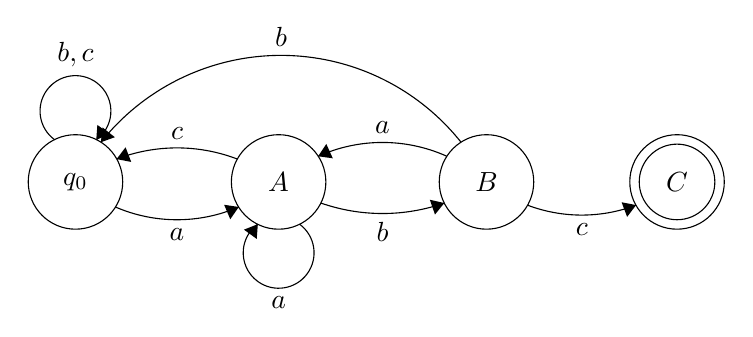
\begin{tikzpicture}[scale=0.2]
\tikzstyle{every node}+=[inner sep=0pt]
\draw [black] (16.6,-30.5) circle (3);
\draw (16.6,-30.5) node {$q_0$};
\draw [black] (29.5,-30.5) circle (3);
\draw (29.5,-30.5) node {$A$};
\draw [black] (42.7,-30.5) circle (3);
\draw (42.7,-30.5) node {$B$};
\draw [black] (54.8,-30.5) circle (3);
\draw (54.8,-30.5) node {$C$};
\draw [black] (54.8,-30.5) circle (2.4);
\draw [black] (15.277,-27.82) arc (234:-54:2.25);
\draw (16.6,-23.25) node [above] {$b,c$};
\fill [black] (17.92,-27.82) -- (18.8,-27.47) -- (17.99,-26.88);
\draw [black] (40.024,-31.838) arc (-70.68221:-109.31779:11.861);
\fill [black] (40.02,-31.84) -- (39.1,-31.63) -- (39.43,-32.57);
\draw (36.1,-33.01) node [below] {$b$};
\draw [black] (52.201,-31.974) arc (-69.26268:-110.73732:9.745);
\fill [black] (52.2,-31.97) -- (51.28,-31.79) -- (51.63,-32.72);
\draw (48.75,-33.11) node [below] {$c$};
\draw [black] (32.007,-28.874) arc (114.31851:65.68149:9.938);
\fill [black] (32.01,-28.87) -- (32.94,-29) -- (32.53,-28.09);
\draw (36.1,-27.49) node [above] {$a$};
\draw [black] (18.215,-27.978) arc (141.48882:38.51118:14.614);
\fill [black] (18.21,-27.98) -- (19.1,-27.66) -- (18.32,-27.04);
\draw (29.65,-21.96) node [above] {$b$};
\draw [black] (30.823,-33.18) arc (54:-234:2.25);
\draw (29.5,-37.75) node [below] {$a$};
\fill [black] (28.18,-33.18) -- (27.3,-33.53) -- (28.11,-34.12);
\draw [black] (26.969,-32.089) arc (-66.58879:-113.41121:9.864);
\fill [black] (26.97,-32.09) -- (26.04,-31.95) -- (26.43,-32.87);
\draw (23.05,-33.4) node [below] {$a$};
\draw [black] (19.214,-29.049) arc (111.00052:68.99948:10.702);
\fill [black] (19.21,-29.05) -- (20.14,-29.23) -- (19.78,-28.3);
\draw (23.05,-27.84) node [above] {$c$};
\end{tikzpicture}
\end{center}

Formally this machine is defined by:
\begin{itemize}
\item $Q=\{q_0,A,B,C\}$.
\item $\Sigma=\{a,b,c\}$.
\item $\delta:\begin{cases}
(q_0,a)\mapsto A\\
(q_0,b)\mapsto q_0\\
(q_0,c)\mapsto q_0\\
(A,a)\mapsto A\\
(A,b)\mapsto B\\
(A,c)\mapsto q_0\\
(B,a)\mapsto A\\
(B,b)\mapsto q_0\\
(B,c)\mapsto C\\
 \end{cases}$
\item $q_0$ (the starting state).
\item $H=\{C\}$ (the set of halt states).
\end{itemize}
For most people the diagrams of simple FSMs are much easier to understand than their formal definitions, so usually we will just give diagrams and omit the formal definition of $\delta$. 
\end{example}
        


\subsection{Turing Machines}
Finite state machines are useful, but they are quite limited. There are many things they can't do, even in the context of abstract computation. For example, you can't write an FSM to check if graphs are connected (even if you write it so that you can define graphs using input strings). You can't write an FSM to check if a given set of polynomial equations has a solution. You can't even write an FSM to add two arbitrary binary numbers together!

\begin{exercise}
Prove informally that no FSM exists that can add two arbitrary binary numbers together. 
\end{exercise}

Many of the limitations of FSMs, at least as far as abstract computation is concerned, come down to the fact that they can only record the inputs they have received by changing their state, and since they only have a finite number of states this translates into only having a limited amount of memory. Similarly, the only way an FSM can output information is via the state it's in when it stops computing. Now, real world computers also have finite memory, but this amount of memory is dependent on current technology and is increasing all the time. Theoretical computer scientists often prefer to study abstract computation by assuming memory is infinite, which leads us to...

\begin{definition}[Turing Machine]
A Turing machine (TM) is an abstract machine composed of a set of states and an input language (like an FSM), an infinite tape consisting of spaces where symbols can be written, a tape head that at any given time is reading some part of the tape, a distinguished set of states (denoting halting, possibly with different states denoting success/acceptance or failure/rejection), and a function that says what happens to the machine if it is in a particular state reading a particular symbol. Unlike an FSM a Turing machine can write on its tape, and the tape head can move forward and backwards along it. This ability to write and review what has been written gives the TM a theoretically infinite amount of memory. 

Formally we define a TM to consist of the following seven things:
\begin{enumerate}
\item A finite set of states $Q$.
\item A finite alphabet $\Sigma$. In addition to the symbols in $\Sigma$, a TM uses the additional special symbols $\tvs$ and $:$. We use $\tvs$ to represent blank spaces on the tape, and we use $:$ to denote the very first symbol on the tape (and nothing else!).
\item A one way infinite tape consisting of numbered squares starting at $0$. Each square contains one symbol from $\Sigma\cup\{\tvs,:\}$. A square contains $:$ if and only if it is square $0$. We think of $\tvs$ as denoting `empty' squares.
\item A tape head that moves up and down the tape reading symbols. 
\item A distinguished starting state $q_0$.
\item A set $H\subseteq Q$ of halting states (maybe partitioned into `accept' states and `reject' states).
\item A function $\delta: (Q\setminus H)\times\Sigma\cup\{\tvs,:\} \to Q \times (\Sigma\cup\{\tvs,\rightarrow,\leftarrow\})$. I.e. this function is defined for all pairs of non-halting states and symbols from $\Sigma\cup\{\tvs,:\}$. The output is the new state of the machine and an action for the tape head (the arrows represent moving the tape head one square to the right or the left, and symbols from $\Sigma\cup\{\tvs\}$ mean the tape head should replace the current contents of that square with the new symbol).
\end{enumerate}

The function $\delta$ has the following additional restriction. If the tape head is reading $:$ then the action of the tape head must be to move to the right (i.e. it must be $\rightarrow$) . This is so the tape head never falls off the initial end of the tape. Formally we express this by saying that for all $q\in 
Q$ we have $\delta(q,:)=(q',\rightarrow)$ for some $q'\in Q$ (note of course that the exact value of $q'$ depends on $q$).

Since every TM has a tape and tape head we can specify a given TM using the $5$-tuple $(Q,\Sigma,q_0,H,\delta)$.
\end{definition}   

A Turing machine starts in the special start state with the tape head reading the first square of the tape (which must contain the symbol $:$). The initial state of the tape is considered to be the \emph{input}. We assume that the input will always be $:$ followed by a finite sequence of characters from $\Sigma$, followed by an infinite number of $\tvs$ symbols.   
 
A \emph{run} of a Turing machine on input $I$ is a sequence of abstract triples representing the state the machine is in, the position of the tape head, and the current state of the tape. A run is completely determined by the input $I$ on the tape and the function $\delta$. At each step the machine reads the symbol from the square the tape head is reading, checks its current state and uses $\delta$ to figure out what to do next. Depending on $\delta$ it may or may not change state, and it will either replace the symbol in the square under the tape head with a new one, or move the tape head left or right. 

Since we have assumed the tape head starts on the first square, and the first square contains $:$, the first move will always be for the tape head to move to the right. The run \emph{halts} if the TM gets to one of its halt states (in which case the sequence representing the run is finite).  We say a Turing machine \emph{accepts} if its run ends in a halt state we have decided corresponds to acceptance, and \emph{rejects} if it ends in a halt state we have decided corresponds to rejection. Sometimes we want the TM to output something, in which case we consider the contents of the tape up to the first blank when it gets to an accept state as the output. We often use the notation $T(x)$ to denote the action, or output, of Turing machine $T$ on input $x$.


\begin{example}[Unary addition of $1$]
Let $\Sigma=\{1\}$. This machine adds one to a natural number represented in unary notation.
\begin{center}
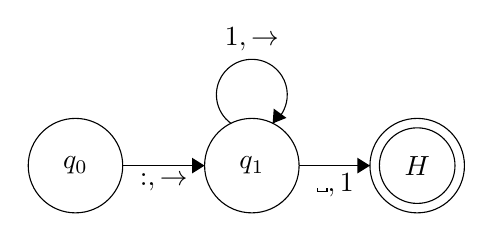
\begin{tikzpicture}[scale=0.2]
\tikzstyle{every node}+=[inner sep=0pt]
\draw [black] (3.3,-34.6) circle (3);
\draw (3.3,-34.6) node {$q_0$};
\draw [black] (14.5,-34.6) circle (3);
\draw (14.5,-34.6) node {$q_1$};
\draw [black] (25,-34.6) circle (3);
\draw (25,-34.6) node {$H$};
\draw [black] (25,-34.6) circle (2.4);
\draw [black] (6.3,-34.6) -- (11.5,-34.6);
\fill [black] (11.5,-34.6) -- (10.7,-34.1) -- (10.7,-35.1);
\draw (8.9,-35.1) node [below] {$:,\rightarrow$};
\draw [black] (17.5,-34.6) -- (22,-34.6);
\fill [black] (22,-34.6) -- (21.2,-34.1) -- (21.2,-35.1);
\draw (19.75,-35.1) node [below] {$\tvs,1$};
\draw [black] (13.177,-31.92) arc (234:-54:2.25);
\draw (14.5,-27.35) node [above] {$1,\rightarrow$};
\fill [black] (15.82,-31.92) -- (16.7,-31.57) -- (15.89,-30.98);
\end{tikzpicture}
\end{center}
\end{example}

\begin{example}[Unary addition of two natural numbers]
This machine uses the alphabet $\{1,*\}$ and correct input is of form $*,a*,*b,a*b$ followed by blanks  ($a$ and $b$ are strings containing only $1$). Here $a$ and $b$ represent the numbers to be added together in unary notation. Output is the unary number that is left on the tape when the machine accepts. 
\begin{center}
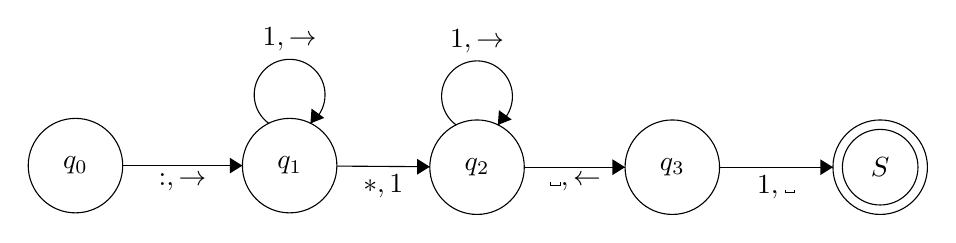
\begin{tikzpicture}[scale=0.2]
\tikzstyle{every node}+=[inner sep=0pt]
\draw [black] (10.5,-19.2) circle (3);
\draw (10.5,-19.2) node {$q_0$};
\draw [black] (24.1,-19.2) circle (3);
\draw (24.1,-19.2) node {$q_1$};
\draw [black] (36,-19.3) circle (3);
\draw (36,-19.3) node {$q_2$};
\draw [black] (48.4,-19.3) circle (3);
\draw (48.4,-19.3) node {$q_3$};
\draw [black] (61.6,-19.3) circle (3);
\draw (61.6,-19.3) node {$S$};
\draw [black] (61.6,-19.3) circle (2.4);
\draw [black] (13.5,-19.2) -- (21.1,-19.2);
\fill [black] (21.1,-19.2) -- (20.3,-18.7) -- (20.3,-19.7);
\draw (17.3,-19.7) node [below] {$:,\rightarrow$};
\draw [black] (27.1,-19.23) -- (33,-19.27);
\fill [black] (33,-19.27) -- (32.2,-18.77) -- (32.2,-19.77);
\draw (30.05,-19.76) node [below] {$*,1$};
\draw [black] (22.777,-16.52) arc (234:-54:2.25);
\draw (24.1,-11.95) node [above] {$1,\rightarrow$};
\fill [black] (25.42,-16.52) -- (26.3,-16.17) -- (25.49,-15.58);
\draw [black] (34.677,-16.62) arc (234:-54:2.25);
\draw (36,-12.05) node [above] {$1,\rightarrow$};
\fill [black] (37.32,-16.62) -- (38.2,-16.27) -- (37.39,-15.68);
\draw [black] (39,-19.3) -- (45.4,-19.3);
\fill [black] (45.4,-19.3) -- (44.6,-18.8) -- (44.6,-19.8);
\draw (42.2,-19.8) node [below] {$\tvs,\leftarrow$};
\draw [black] (51.4,-19.3) -- (58.6,-19.3);
\fill [black] (58.6,-19.3) -- (57.8,-18.8) -- (57.8,-19.8);
\draw (55,-19.8) node [below] {$1,\tvs$};
\end{tikzpicture}
\end{center}

Note that strictly speaking the $\delta$ represented by this diagram isn't a function. This is not a problem because all state/input combinations not on the diagram can be considered to map to an undrawn reject state, so the machine rejects if it gets input of an incorrect form. The machine is guaranteed (hopefully) to work correctly when the input has the correct form.

\end{example}



Because we demand that $\delta$ is a function, the only way a run of a TM can stop is by the machine entering one of the halt states. A run of a TM may not halt! 

\begin{exercise}
Design a Turing machine using the alphabet $\Sigma=\{0,1\}$ that does not halt for any input.
\end{exercise}



\subsection{Decision Problems}
Turing machines are important because they are closely related to a special kind of question called a \emph{decision problem}. Decision problems are things like
\begin{enumerate}
\item Given a graph $G$, is $G$ connected?
\item Does a given string of English characters contain the word \emph{biscuits} as a substring?
\item Is a given propositional formula satisfiable?
\item Is a given natural number prime?
\end{enumerate}

The answer to all these questions is either yes or no (depending on the graph/string etc. we are given). An answer always exists in theory, though we may not know how to find it. A decision problem has a generic component (the question), and a specific instance (the particular object we are asking the question about). For example, the generic component of the first question is whether a graph is connected, and the specific instance is whatever specific graph we are given. The generic component of the second question is whether a string contains the word \emph{biscuits}, and the specific instance is the particular string we are given. The result of applying the generic question to a specific instance will be either yes or no.

More abstractly a decision problem is a set of objects that can be partitioned into two, with one of the sets representing the objects for which the answer is \emph{yes}, and the other representing the objects for which the answer is \emph{no}. We usually say the set of all objects is the set of \emph{instances} of the problem, and that the two subsets partition the set of instances into \emph{yes instances} and \emph{no instances}. Looking again at our 2nd example, here the instance set is the set of all strings of English characters, the yes instances are those strings containing the word \emph{biscuits}, and the no instances are those not containing it. E.g. \emph{jhbybiscuitslp} is a yes instance, and \emph{bsjsppojlkn} is a no instance. 


\subsection{Formal Languages}
To connect Turing machines and decision problems we need to be able to represent decision problems in a formal language. That is we need to \emph{encode} the instances of the problem using the symbols from a finite alphabet. That is, we want to find an alphabet so that every instance of the problem is represented by a string of finite length, and distinct instances have distinct strings (abstractly we want a 1-1 map from the set of instances to the set of finite strings over some finite alphabet). Recall the following definitions and facts:
\begin{itemize}
\item A (finite) alphabet $\Sigma$ is a finite set of symbols, e.g. $\{a,b,c\}$,\\ or $\{0,1,2,3,4,5,6,7,8,9\}$.
\item A string over $\Sigma$ is a sequence of characters, e.g. 01001, or the digits of $\pi$.
\item The \emph{length} of a string is the number of characters it contains. Given a string $s$ we use $|s|$ to denote the length of $s$. E.g $|01001|=5$, and the length of the string defined by the digits of $\pi$ is $\omega$ (this symbol means countably infinite).
\item The string with no elements is called the \emph{empty string}. We denote it using $\epsilon$, and $|\epsilon|=0$ by definition.
\item If $a=a_1\ldots a_m$ and $b=b_1\ldots b_n$ are strings over the same alphabet then we can \emph{concatenate} them to get $ab=a_1\ldots a_m b_1\ldots b_n$. Note that $|ab|=|a|+|b|$.
\item For all strings $a$ we have $\epsilon a = a$, and for all finite length $a$ we have $a\epsilon=a$.
\item The set of all finite length strings over $\Sigma$ is denoted by $\Sigma^*$.
\item A \emph{formal language} over $\Sigma$ is a subset of $\Sigma^*$.
\item If $L$ is a formal language over $\Sigma$ then we can define the characteristic function of $L$ by $\chi_L:\Sigma^*\to\{0,1\}$ and $\chi_L(s) = \begin{cases}1 \text{ if } s\in L \\
0 \text{ if } s\notin L \end{cases}$   
\end{itemize}

\begin{definition}[encoding scheme]
If $\Sigma$ is a finite alphabet, $D$ is a decision problem, and $I_D$ is the set of all instances of $D$, an encoding scheme for $D$ using $\Sigma$ is a function $\mathbf{code}: I_D\to \Sigma^*$ such that:
\begin{enumerate}
\item if $x,y\in I_D$ and $x\neq y$ we must have $\mathbf{code}(x)\neq \mathbf{code}(y)$ (i.e. $\mathbf{code}$ is $1-1$),
\item it is possible to work out if a string in $\Sigma^*$ is $\mathbf{code}(x)$ for some $x\in I_D$, and 
\item the process for converting $x$ to $\mathbf{code}(x)$ and $\mathbf{code}(x)$ to $x$ is well defined. 
\end{enumerate}
\end{definition}

Using encoding we can turn decision problems into formal languages as follows.
\begin{definition}[$L_D$]\label{D:LD}
Given a decision problem $D$, a finite alphabet $\Sigma$, and an encoding for $D$ using $\Sigma$, the language defined by $D$ is the set $L_D=\{\textbf{code}(x):x$ is a yes instance of $D\}$.
\end{definition}

So, if we encode $D$ using $\Sigma$, the set $\Sigma^*$ will be partitioned into three subsets: the set of codes of the yes instances ($L_D$), the set of codes of the no instances, and the set of strings that are not the code of any instance of $D$. 

Definition \ref{D:LD} shows us how an encodable decision problem $D$ defines a formal language $L_D$, and the problem of deciding whether an instance of $D$ is `yes' or `no' is equivalent to the problem of deciding whether the code of that instance is in $L_D$ or not. This also works in reverse in the obvious way. Any formal language $L$ defines a decision problem $D_L$ of the form ``is this word from $\Sigma^*$ in $L$?". 


\subsection{Turing Machines and Decision Problems}
We can now discuss the relationship between Turing machines and decision problems. 

\begin{definition}[Decidable]\label{D:dec}
An (encodable) decision problem $D$ is decidable if there is a Turing machine $T$ that accepts when its input is the code of a yes instance of $D$, and rejects when its input is the code of a no instance (or not the code of an instance at all). We say $T$ decides $D$.
\end{definition}

The obvious question now is, ``Is every decision problem that can be encoded using a finite alphabet decidable?" Many people intuitively felt that the answer should be yes, but it turns out the answer is actually no. We will prove this later. Studying the kinds of decision problems that cannot be decided by a Turing machine is the focus of a large part of this course. For now we make another definition.

\begin{definition}[Semidecidable]\label{D:semidec}
An (encodable) decision problem $D$ is semidecidable if there is a Turing machine $T$ that accepts when its input is the code of a yes instance of $D$, and does not halt (i.e. it runs forever) when its input is the code of a no instance (or not the code of an instance at all). We say $T$ semidecides $D$.
\end{definition}  

It turns out that some encodable decision problems are not even semidecidable, and we also prove this later. We saw in the previous section that encodable decision problems are equivalent to formal languages, and there are versions of definitions \ref{D:dec} and \ref{D:semidec} that apply to languages.


\begin{exercise}
Prove that every decidable decision problem is also semidecidable.
\end{exercise}

\begin{definition}[Recursive]
A formal language $L$ over a finite alphabet $\Sigma$ is recursive if there is a Turing machine $T$ that takes input $x$ from $\Sigma^*$ and accepts when $x\in L$ and rejects when $x\notin L$.  
\end{definition}

\begin{definition}[Recursively enumerable]
A formal language $L$ over a finite alphabet $\Sigma$ is recursively enumerable if there is a Turing machine $T$ that takes input $x$ from $\Sigma^*$ and accepts when $x\in L$ and runs forever when $x\notin L$. We often shorten \emph{recursively enumerable} to \emph{r.e.}).  
\end{definition}

By definition of $L_D$ and $D_L$ we have the following correspondences for encodable decision problems:
\begin{align*}
D \text{ is decidable}&\iff L_D \text{ is recursive}\\
D_L \text{ is decidable}&\iff L \text{ is recursive}\\
D \text{ is semidecidable}&\iff L_D \text{ is recursively enumerable}\\
D_L \text{ is semidecidable}&\iff L \text{ is recursively enumerable}\\
\end{align*} 

\begin{example}[Palindromes]
Let $\Sigma=\{a,b\}$. This TM takes as input finite strings from $\Sigma^*$ and accepts if they are palindromes (i.e. if they are the same forwards and backwards ,e.g. $abbabba$), and rejects if they are not. I.e. it proves that the set of palindromes using $a$ and $b$ is recursive.

\begin{center}
\resizebox{\columnwidth}{!}{%
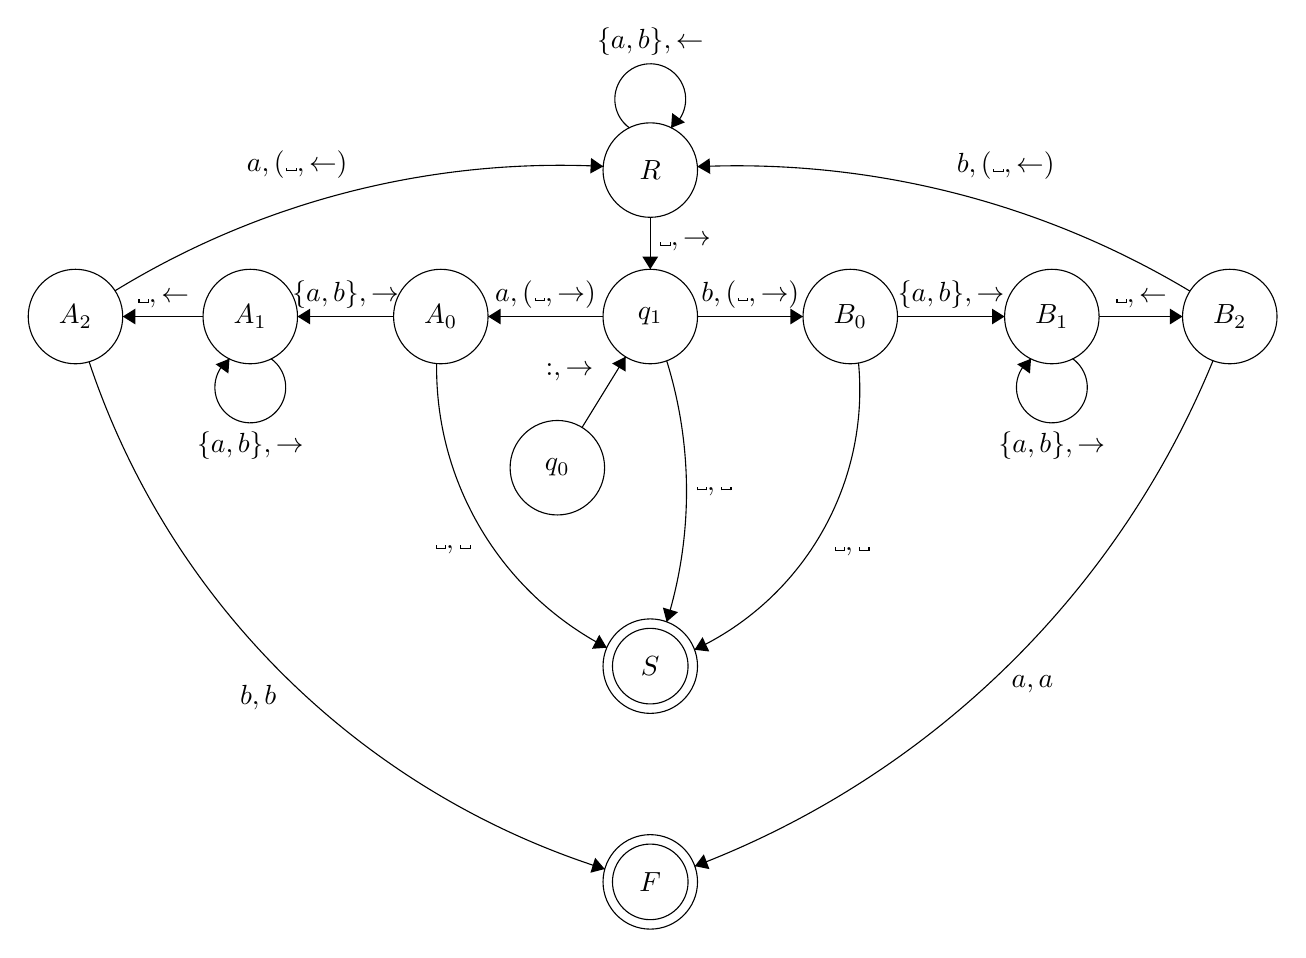
\begin{tikzpicture}[scale=0.2]
\tikzstyle{every node}+=[inner sep=0pt]
\draw [black] (39.6,-15.5) circle (3);
\draw (39.6,-15.5) node {$q_1$};
\draw [black] (52.3,-15.5) circle (3);
\draw (52.3,-15.5) node {$B_0$};
\draw [black] (65.1,-15.5) circle (3);
\draw (65.1,-15.5) node {$B_1$};
\draw [black] (76.4,-15.5) circle (3);
\draw (76.4,-15.5) node {$B_2$};
\draw [black] (26.3,-15.5) circle (3);
\draw (26.3,-15.5) node {$A_0$};
\draw [black] (14.2,-15.5) circle (3);
\draw (14.2,-15.5) node {$A_1$};
\draw [black] (3.1,-15.5) circle (3);
\draw (3.1,-15.5) node {$A_2$};
\draw [black] (33.7,-25.1) circle (3);
\draw (33.7,-25.1) node {$q_0$};
\draw [black] (39.6,-6.2) circle (3);
\draw (39.6,-6.2) node {$R$};
\draw [black] (39.6,-51.4) circle (3);
\draw (39.6,-51.4) node {$F$};
\draw [black] (39.6,-51.4) circle (2.4);
\draw [black] (39.6,-37.7) circle (3);
\draw (39.6,-37.7) node {$S$};
\draw [black] (39.6,-37.7) circle (2.4);
\draw [black] (42.6,-15.5) -- (49.3,-15.5);
\fill [black] (49.3,-15.5) -- (48.5,-15) -- (48.5,-16);
\draw (45.95,-15) node [above] {$b,(\tvs,\ra)$};
\draw [black] (55.3,-15.5) -- (62.1,-15.5);
\fill [black] (62.1,-15.5) -- (61.3,-15) -- (61.3,-16);
\draw (58.7,-15) node [above] {$\{a,b\},\ra$};
\draw [black] (68.1,-15.5) -- (73.4,-15.5);
\fill [black] (73.4,-15.5) -- (72.6,-15) -- (72.6,-16);
\draw (70.75,-15) node [above] {$\tvs,\la$};
\draw [black] (36.6,-15.5) -- (29.3,-15.5);
\fill [black] (29.3,-15.5) -- (30.1,-16) -- (30.1,-15);
\draw (32.95,-15) node [above] {$a,(\tvs,\ra)$};
\draw [black] (23.3,-15.5) -- (17.2,-15.5);
\fill [black] (17.2,-15.5) -- (18,-16) -- (18,-15);
\draw (20.25,-15) node [above] {$\{a,b\},\ra$};
\draw [black] (11.2,-15.5) -- (6.1,-15.5);
\fill [black] (6.1,-15.5) -- (6.9,-16) -- (6.9,-15);
\draw (8.65,-15) node [above] {$\tvs,\la$};
\draw [black] (35.27,-22.54) -- (38.03,-18.06);
\fill [black] (38.03,-18.06) -- (37.18,-18.48) -- (38.04,-19);
\draw (36.02,-19.02) node [left] {$:,\ra$};
\draw [black] (5.614,-13.863) arc (121.48441:87.10459:54.115);
\fill [black] (36.61,-5.97) -- (35.84,-5.43) -- (35.79,-6.42);
\draw (17.18,-6.76) node [above] {$a,(\tvs,\la)$};
\draw [black] (42.592,-5.984) arc (92.59079:59.04384:55.895);
\fill [black] (42.59,-5.98) -- (43.41,-6.45) -- (43.37,-5.45);
\draw (62.17,-6.81) node [above] {$b,(\tvs,\la)$};
\draw [black] (66.423,-18.18) arc (54:-234:2.25);
\draw (65.1,-22.75) node [below] {$\{a,b\},\ra$};
\fill [black] (63.78,-18.18) -- (62.9,-18.53) -- (63.71,-19.12);
\draw [black] (15.523,-18.18) arc (54:-234:2.25);
\draw (14.2,-22.75) node [below] {$\{a,b\},\ra$};
\fill [black] (12.88,-18.18) -- (12,-18.53) -- (12.81,-19.12);
\draw [black] (38.277,-3.52) arc (234:-54:2.25);
\draw (39.6,1.05) node [above] {$\{a,b\},\la$};
\fill [black] (40.92,-3.52) -- (41.8,-3.17) -- (40.99,-2.58);
\draw [black] (39.6,-9.2) -- (39.6,-12.5);
\fill [black] (39.6,-12.5) -- (40.1,-11.7) -- (39.1,-11.7);
\draw (40.1,-10.85) node [right] {$\tvs,\ra$};
\draw [black] (36.714,-50.583) arc (-107.5108:-161.53957:50.565);
\fill [black] (36.71,-50.58) -- (36.1,-49.87) -- (35.8,-50.82);
\draw (14.7,-38.89) node [below] {$b,b$};
\draw [black] (75.335,-18.304) arc (-22.28191:-69.13662:57.811);
\fill [black] (42.43,-50.4) -- (43.36,-50.59) -- (43,-49.65);
\draw (63.87,-38.25) node [below] {$a,a$};
\draw [black] (36.842,-36.526) arc (-117.36188:-180.78654:20.004);
\fill [black] (36.84,-36.53) -- (36.36,-35.71) -- (35.9,-36.6);
\draw (28.23,-30.3) node [left] {$\tvs,\tvs$};
\draw [black] (52.825,-18.45) arc (5.36879:-64.91413:18.221);
\fill [black] (42.41,-36.66) -- (43.35,-36.77) -- (42.92,-35.86);
\draw (51.16,-30.43) node [right] {$\tvs,\tvs$};
\draw [black] (40.643,-18.311) arc (17.27171:-17.27171:27.917);
\fill [black] (40.64,-34.89) -- (41.36,-34.27) -- (40.4,-33.98);
\draw (42.4,-26.6) node [right] {$\tvs,\tvs$};
\end{tikzpicture}
}
\end{center}

This TM introduces some new shorthand notation. The command `$a,(\tvs,\ra)$' for example signifies ``if reading $a$ write $\tvs$ then move the tape head right", and the command `$\{a,b\},\ra$' means ``if reading either $a$ or $b$ then move the tape head right.
\end{example}

\begin{exercise}
Let $\Sigma=\{1\}$, and let $L$ be the subset of $\Sigma^*$ containing all strings of even length. Prove that $L$ is recursive.
\end{exercise}


\subsection{Pushdown Automata}
As we have discussed, Turing machines are strictly more powerful than FSMs due to them effectively having infinite memory. This means there are tasks we can design a TM to perform that can not be done by an FSM. At this point we may be curious if there's a model of computation between FSMs and TMs. It turns out the answer is yes. A \emph{pushdown automaton} is another abstract computation system based on FSMs. Unlike an FSM, a pushdown automaton also has access to infinite memory in the form of a stack. In addition to reading input a pushdown automaton also has access to the top element of the stack, and its $\delta$ function takes this information into account. Pushdown automata not only change state but may also manipulate the stack. It turns out that this makes them strictly more powerful than FSMs, but strictly less powerful than Turing machines. However, pushdown automata with two stacks turn out to be equivalent to Turing machines, because we can use one stack to model the part of the tape to the left of the tape head, and the other to model the part of the tape to the right.    


\subsection{Computation and Language}
\begin{definition}[Recognize]
Let $M$ be an abstract machine capable of acting on input from $\Sigma^*$ for a finite alphabet $\Sigma$, and let $L\subseteq\Sigma^*$ be a language. We say $M$ recognizes $L$ if $M$ accepts on input $x$ if and only if $x\in L$. 
\end{definition}

According to this definition, every recursively enumerable language has a Turing machine that recognizes it (this is just the definition of r.e.). Moreover, every Turing machine $T$ defines a recursively enumerable language (just take the set of all $x$ such that $T(x)$ halts). This gives us a correspondence between the class of Turing machines and the class of r.e. languages.

\begin{theorem}
The class of recursively enumerable languages is precisely the class of languages that can be recognized by a Turing machine.
\end{theorem}

This is similar to the result that says that regular languages are precisely those that can be recognized by an FSM. Indeed, the connection between models of computation and formal languages is very strong, and we see this in the \emph{Chomsky hierarchy} (see figure \ref{F:chom}). The characterization of regular languages as those recognizable by an FSM, for example, gives us useful things like the \emph{pumping lemma} very easily (if you don't know what this is look it up!).

\begin{figure}[h]
\begin{center}
\begin{tabular}{ |c| c | }
 \hline \textbf{language} & \textbf{model of computation} \\ \hline
 recursively enumerable & Turing machines \\ \hline 
 context-sensitive & linear bounded automata \\ \hline
 context-free & pushdown automata \\ \hline
 regular & finite state machines\\ \hline
\end{tabular}
\end{center}
\caption{The Chomsky hierarchy of formal languages and their associated models of computation. Models of computation are arranged in order of power. On this course we are mainly interested in Turing machines. Note that it is possible to refine this hierarchy by adding extra classes, and this may result in something that is not linearly ordered.}
\label{F:chom}
\end{figure}



\end{document}
\subsection{Exercises}
\documentclass{article}

\usepackage{amsmath, mathrsfs, amssymb, stmaryrd, cancel, relsize,tikz,amsthm,comment,enumerate}

\theoremstyle{definition}
\newtheorem{Q}{Question}

\newcommand{\tvs}{\textvisiblespace}
\newcommand{\ra}{\rightarrow}
\newcommand{\la}{\leftarrow}
%\includecomment{comment}

%\pagenumbering{gobble}

\title{ITCS 532 Foundations of Computer Science\\
Week 1 - Models of Computation (Homework)}
\author{Rob Egrot}
\date{}

\begin{document}
\maketitle

\begin{Q}
A quadratic in $x$ over the integers has form $q(x)=ax^2+bx+c$, where $x$ is a variable and $a,b$ and $c$ are integers. Suppose our decision problem is whether a given quadratic over the integers has a root in the integers. So the set of instances is the set of all quadratics over the integers. A quadratic $q$ is a yes instance if there is an integer $z$ such that $q(z)=0$.

Design a suitable encoding system for this decision problem (you don't need to design a Turing machine to solve it!).
\end{Q}
\begin{comment}
\textbf{Solution}
Use $\Sigma = \{1,-,*\}$. Store $a$, $b$ and $c$ in unary, separated by $*$, using $-$ to denote negatives. E.g. we express $2x^2 - 3x +1$ as $11*-111*1$.
\end{comment}

\begin{Q}
Let $\Sigma=\{1,*\}$. Design a Turing machine that accepts as input a unary number (i.e. a finite string containing only 1s), and outputs that number multiplied by 2. E.g. If the input is 111 the output will be 111111. Hint: $*$ does not appear in the input or the output, but we can use it during the process of calculating the output.
\end{Q}
\begin{comment}
\textbf{Solution}
\begin{center}
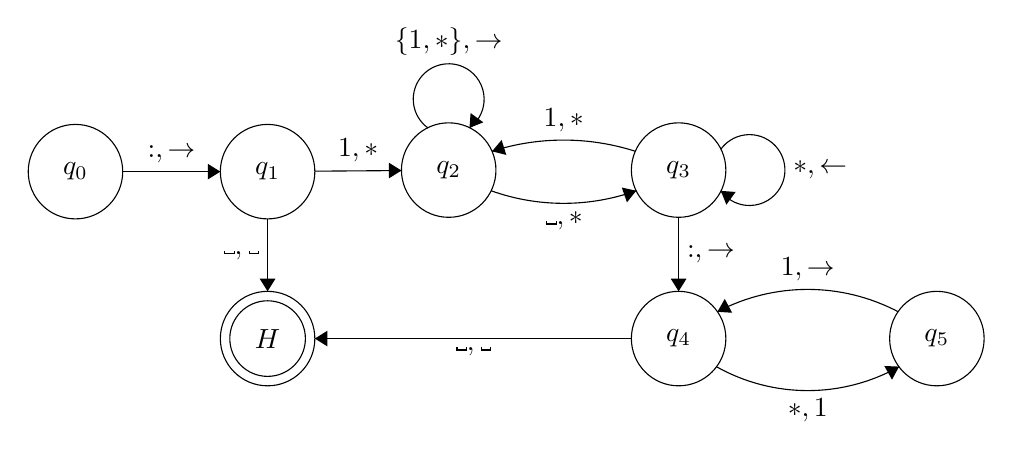
\begin{tikzpicture}[scale=0.2]
\tikzstyle{every node}+=[inner sep=0pt]
\draw [black] (14.6,-15.2) circle (3);
\draw (14.6,-15.2) node {$q_0$};
\draw [black] (26.8,-15.2) circle (3);
\draw (26.8,-15.2) node {$q_1$};
\draw [black] (26.8,-25.8) circle (3);
\draw (26.8,-25.8) node {$H$};
\draw [black] (26.8,-25.8) circle (2.4);
\draw [black] (38.3,-15.1) circle (3);
\draw (38.3,-15.1) node {$q_2$};
\draw [black] (52.9,-15.1) circle (3);
\draw (52.9,-15.1) node {$q_3$};
\draw [black] (52.9,-25.8) circle (3);
\draw (52.9,-25.8) node {$q_4$};
\draw [black] (69.3,-25.8) circle (3);
\draw (69.3,-25.8) node {$q_5$};
\draw [black] (17.6,-15.2) -- (23.8,-15.2);
\fill [black] (23.8,-15.2) -- (23,-14.7) -- (23,-15.7);
\draw (20.7,-14.7) node [above] {$:,\ra$};
\draw [black] (26.8,-18.2) -- (26.8,-22.8);
\fill [black] (26.8,-22.8) -- (27.3,-22) -- (26.3,-22);
\draw (26.3,-20.5) node [left] {$\tvs,\tvs$};
\draw [black] (29.8,-15.17) -- (35.3,-15.13);
\fill [black] (35.3,-15.13) -- (34.5,-14.63) -- (34.5,-15.63);
\draw (32.55,-14.63) node [above] {$1,\ast$};
\draw [black] (36.977,-12.42) arc (234:-54:2.25);
\draw (38.3,-7.85) node [above] {$\{1,\ast\},\ra$};
\fill [black] (39.62,-12.42) -- (40.5,-12.07) -- (39.69,-11.48);
\draw [black] (50.209,-16.412) arc (-70.28917:-109.71083:13.666);
\fill [black] (50.21,-16.41) -- (49.29,-16.21) -- (49.62,-17.15);
\draw (45.6,-17.71) node [below] {$\tvs,\ast$};
\draw [black] (55.58,-13.777) arc (144:-144:2.25);
\draw (60.15,-15.1) node [right] {$\ast,\la$};
\fill [black] (55.58,-16.42) -- (55.93,-17.3) -- (56.52,-16.49);
\draw [black] (52.9,-18.1) -- (52.9,-22.8);
\fill [black] (52.9,-22.8) -- (53.4,-22) -- (52.4,-22);
\draw (53.4,-20.45) node [right] {$:,\ra$};
\draw [black] (66.899,-27.585) arc (-60.64203:-119.35797:11.828);
\fill [black] (66.9,-27.58) -- (65.96,-27.54) -- (66.45,-28.41);
\draw (61.1,-29.6) node [below] {$\ast,1$};
\draw [black] (55.359,-24.095) arc (117.75844:62.24156:12.326);
\fill [black] (55.36,-24.1) -- (56.3,-24.16) -- (55.83,-23.28);
\draw (61.1,-22.18) node [above] {$1,\ra$};
\draw [black] (49.9,-25.8) -- (29.8,-25.8);
\fill [black] (29.8,-25.8) -- (30.6,-26.3) -- (30.6,-25.3);
\draw (39.85,-26.3) node [below] {$\tvs,\tvs$};
\draw [black] (41.046,-13.906) arc (107.74904:72.25096:14.937);
\fill [black] (41.05,-13.91) -- (41.96,-14.14) -- (41.66,-13.19);
\draw (45.6,-12.69) node [above] {$1,\ast$};
\end{tikzpicture}
\end{center}
\end{comment}

\begin{Q}
Can a formal language $L$ exist that is recursive but not r.e.?
\end{Q}
\begin{comment}
\textbf{Solution}
No. We know from the notes that decidable implies semidecidable, and this is just the formal language version of that.
\end{comment}

\begin{Q}
Suppose we define a class $\mathcal C$ of abstract computational devices similar to Turing machines but without the $\la$ command (so the tape head may never move backwards).
\begin{enumerate}[(a)]
\item Give an informal argument for why this model of computation is strictly weaker than that of Turing machines.
\item Would it make any difference if we replaced the $\la$ command with a $-$ command that keeps the tape head in the same place?
\item (Hard) Give a rigorous proof for part (a).
\end{enumerate}
\end{Q}
\begin{comment}
\textbf{Solution}
\begin{enumerate}[(a)]
\item No memory.
\item No. Still no memory. 
\item Consider the problem of checking to see if two strings are the same length. Input is, for example, a string of $1$'s followed by a $*$, followed by another string of $1$'s. Suppose we have a $-$ machine $M$ that solves this problem. Then it has a finite number of states, $n$ say. Consider the set $X$ that contains all strings of $k$ ones followed by a $*$, for $k\in\{1,\ldots,n+1\}$. Since $M$ cannot move its tape head backwards, the state it's in when it gets to the $*$ symbol must store all the information about the length of the first string. As $|X| = n+1$, by the pigeon hole principle there must be (at least) two strings in $X$ such that $M$ is in the same state when it gets to $*$. Call these strings $s*$ and $t*$. Then $M$ should accept $s*s$, but then it must also accept $t*s$, which is incorrect. 
\end{enumerate}
\end{comment}

\end{document}
\newpage

\section{Turing Machine Variants}\label{S:TMvar}
\documentclass{article}

\usepackage{amsmath, mathrsfs, amssymb, stmaryrd, cancel, relsize,tikz,amsthm}

\theoremstyle{plain}
\newtheorem{theorem}{Theorem}[section]{\bfseries}{\itshape}
\newtheorem{proposition}[theorem]{Proposition}{\bfseries}{\itshape}
\newtheorem{definition}[theorem]{Definition}{\bfseries}{\upshape}
\newtheorem{lemma}[theorem]{Lemma}{\bfseries}{\upshape}
\newtheorem{corollary}[theorem]{Corollary}{\bfseries}{\upshape}
\newtheorem{exercise}[theorem]{Exercise}{\bfseries}{\upshape}

\theoremstyle{definition}
\newtheorem{example}[theorem]{Example}{\bfseries}{\upshape}

\newcommand{\tvs}{\textvisiblespace}
\newcommand{\ra}{\rightarrow}
\newcommand{\la}{\leftarrow}


\title{ITCS 532 Foundations of Computer Science\\
Class 2 - Turing Machine Variants}
\author{Rob Egrot}
\date{}

\begin{document}
\maketitle
\subsection{Multi-tape Turing Machines}
A standard Turing machine has only one tape. We could change the definition so that the machine has two, or even more. Each tape would have its own tape head, though the machine would just have one global state, and the tape heads could move up and down their separate tapes reading and writing independently. Intuitively we might expect that this would give us a more powerful model of computation than single-tape TMs. In other words, that TMs with more than one tape could decide more problems and recognize more languages than their single-tape counterparts. It turns out that this is \emph{not} the case. Multi-tape TMs are equivalent to single-tape TMs, at least as far as decision problems go, in the sense that for any multi-tape TM there's a single-tape TM that gets the same result for the same input. I.e. it will produce the same output, and/or halt in the same state, or run forever if necessary. This is not obvious, but we prove it in theorem \ref{T:multi} below.

\begin{definition}[$k$-tape Turing machine]
A $k$-tape Turing machine $M_k$ is a modified TM with the following additional properties:
\begin{itemize}
\item $M_k$ has $k$ one-way infinite tapes and $k$ independent tape heads. The individual tapes have the same constraints as in the single-tape case.
\item At any moment $M_k$ is in a state $q$. I.e. all tape heads share a single state.
\item We formally describe $M_k$ as a $5$-tuple $(Q,\Sigma,q_0,H,\delta)$. This is just like a normal TM, except that $\delta$ is now defined as 
\begin{equation*}\delta:(Q\setminus H)\times (\Sigma\cup\{\tvs,:\})^k\to Q\times (\Sigma\cup \{\tvs,\la,\ra\})^k\end{equation*}
In other words, $\delta$ has to account for the extra tapes. As in the single-tape case, whenever a tape head reads $:$ the tape head must move right.
\item One tape (call it tape 1) is the designated input tape, and all other tapes are considered to be blank (except for the $:$ symbol at the beginning). The tape heads all start reading the $:$ symbol in the first square of their tape.
\item At each step every tape head reads the symbol on its tape at its position and the tape heads act and the global state changes as determined by $\delta$.
\item Tape 1 is also the output tape. When and if $M_k$ accepts, the output is defined to be the string on tape 1 between $:$ and the first $\tvs$.
\end{itemize}
\end{definition}

\begin{theorem}\label{T:multi}
If $\Sigma$ is a finite alphabet and $M$ is a $k$-tape TM using $\Sigma$ there is a finite alphabet $\Sigma'\supseteq\Sigma$ and a single-tape Turing machine $M'$ using $\Sigma'$ such that for all $x\in \Sigma^*$ we have $M(x)=M'(x)$.  
\end{theorem}
\begin{proof}
The idea is to represent the state of all the tapes, and the positions of all the tape heads, on one tape. To do this we need to expand the alphabet $\Sigma$ considerably. Before we make a formal definition we'll look at an example with two tapes.

\[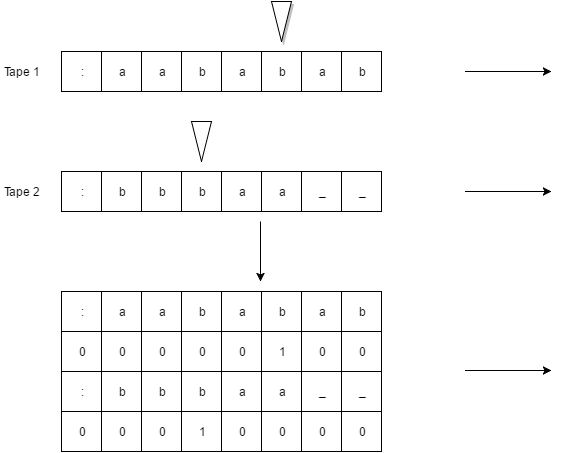
\includegraphics[scale = 0.7]{dMulti.png}\]  

In this example the two tapes of the machine are shown at some point in the run (assume the parts of the tapes out of the picture are blank), along with the positions of the tape heads. The lower part of the picture demonstrates how we would represent this information using only one tape. The symbols of the new tape are represented by the \emph{columns} in the picture. For example, the column 
\[ \left| \begin{array}{c}
b\\1\\a\\0 \end{array} \right| \]
in the 6th position represents that the symbol $b$ is at position 6 on the 1st tape and the 1st tape head is reading that square, and the symbol $a$ is at position 6 on the 2nd tape but the 2nd tape head is somewhere else. 

So, to formally define $\Sigma'$ we need to think about what the possibilities are for the contents of each tape at an arbitrary square, and combine it with the fact that the tape head may or may not be there.  Remember that the very start of the tape contains only the symbol $:$, by definition. The rest of the tape will be used to model the tapes of the multiple tape machine. We will call the start of the tape of single tape machine square -1. We do this because then for $n\geq 0$, square $n$ on the single tape machine corresponds to square $n$ on each tape of the multiple tape machine. In any square other than square 0 (which is a special case as only $:$ can be written there on each tape of the multiple tape machine), there are $|\Sigma\cup\{\tvs\}|$ possibilities for each tape, and for each tape the tape head may or not be present, so we need $(|\Sigma|+1)^k\times 2^k$ symbols to cover all these possible combinations. In addition we need $2^k$ extra symbols for square 0, where only $:$ can be written on each tape but the tape head may or may not be present. Finally we also need every symbol from $\Sigma$ (so that $\Sigma\subset \Sigma'$). So we need $((|\Sigma|+1)^k+1)\times 2^k+|\Sigma|$ symbols in $\Sigma'$.

Anyway, now we know how to represent the state of the tapes of a multi-tape TM using only one tape and an extended alphabet, but we need to work out how to use it simulate the action of the original multi-tape machine. How this works is much too complicated for us to draw using a state change diagram, but we can describe it using high level concepts. So, remember that $M$ is our $k$-tape TM and we are trying to construct a single-tape Turing machine $M'$ using the symbols from $\Sigma'$ so that $M(x)=M'(x)$ for all $x\in \Sigma^*$. To make things easier we set $k=2$. The general case has the same logic. Our machine $M'$ works like this (given input $x$):

\begin{enumerate}
\item $M'$ scans the input $x$ and rewrites $x$ using composite symbols. E.g. $aba\tvs$ will become 
\[ \begin{array}{cccc}
: & a & b & a  \\
1 & 0 & 0 & 0 \\
: & \tvs & \tvs & \tvs  \\
1 & 0 & 0 & 0 
\end{array} \] 
The tape of  $M'$ now represents the initial configuration of $M$ with input $x$. 
\item $M'$ scans the tape till it finds the 1 representing the position of the first tape head. $M'$ changes state to record the symbol the 1st tape head would be reading. $M'$ needs many more states that $M$ to do this, as it must `remember' the state $M$ should be in, and also the current symbol being read by every tape head, and also execute its own program.
\item $M'$ scans the tape for the 1 representing the position of the 2nd tape head and changes state to record the symbols written on the first and second tapes at the appropriate places. 
\item Based on the recorded information about the current symbols being read and the simulated state of $M$ (which $M'$ stores via its own state), $M'$ rewrites the tape to represent $M$ acting on all its tapes.
\item Steps 2, 3, and 4 repeat till $M$ would enter a halting state (if this ever happens!), at which point we proceed to either 6 or 7, depending on the kind of halting state:
\item (Acceptance) $M'$ rewrites the tape so that the output as written on the top row of the combined tape is now written using symbols from $\Sigma$ (so it matches the output of $M$). 
\item (Rejection) $M'$ enters a rejection state.
\end{enumerate}     
\end{proof}

\begin{exercise}
Why is it easy to model a single-tape TM using a multi-tape machine?
\end{exercise}
     


\subsection{The Church-Turing Thesis}
Adding extra tapes is not the only way we can try to extend Turing machines, but it turns out that it's (probably) impossible to design a machine more powerful (in the sense of being able to solve decision problems) than a Turing machine without going beyond the bounds of algorithmic methods. This only applies to situations where you don't care about how long the machine takes. You can design TM variants that can solve problems \emph{faster} than regular TMs, but you can't (it seems) design one capable of solving problems that regular TMs can't. Let's look at some examples.

\begin{example}[Turing machines with a two-way infinite tape] The tape of a regular TM is only infinite in one direction. What if we modified the definition to allow the tape to be infinite in both directions? Would this be a more powerful model of computation? It turns out no. This is fairly easy to see if you think about the multi-tape example. A two-way infinite tape with only one head is at most as powerful as a TM with two tapes and two tape heads. But we saw that this has the same power as a regular TM. Since a TM with a two-way infinite tape is certainly not \emph{less} powerful than a regular TM, they must be equivalent. 
\end{example}

\begin{example}[Turing machines with more than one tape head] We could modify the definition of a Turing machine so that there are two (or more) tape heads working on the same tape. This is slightly tricky to formally define because we have to deal with the possibility of the heads writing in the same space at the same time, but would it give us more power? Again, no. It turns out we can simulate a multi-head TM using a regular TM in a similar way to how we simulated the multi-tape TM. For example, we add symbols to the language so we can model the tape and the positions of the various tape heads on a single tape. For example:

\[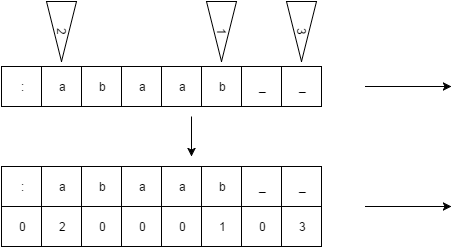
\includegraphics[scale = 0.5]{dMH.png} \]    
\end{example}

\begin{example}[Turing machines operating on a grid] How about instead of a tape we have an infinite grid that the tape head moves around on in two dimensions? Again this is not more powerful. To see this we first model the 2D grid as a sequence of squares in one dimension. This is similar to how we showed the rational numbers are countable. Then we have to create enough states and design the code well enough to deal with the fact that moving the tape head is more complicated now. It's tricky but it can be done.
\end{example}

\begin{exercise}
Prove that the rational numbers $\mathbb{Q}$ are countable.
\end{exercise}

\begin{example}[Turing machines with infinite states] Regular Turing machines can only have a finite number of states. How about if we allow the machine to have an infinite number of states? It turns out that yes, this is more powerful. In fact it's too powerful! If we're allowed to use an infinite number of states then every language over a countable alphabet can be decided by a TM. This is because with an infinite number of states we can have one unique state for every possible input, so all we have to do to `decide' a language is assign acceptance or rejection to each state appropriately. Having an infinite number of states is cheating though, because it's going beyond the realms of computation and into the realm of magic where we can just `guess' the correct answer without having to solve the problem with an algorithm at all.   
\end{example}

People have thought about this very hard, and for a long time, but no one has been able to find a problem for which there is an algorithmic solution that couldn't be abstractly modeled by Turing machines. This leads us to:
\newline
\newline

\begin{centering} \textbf{The Church-Turing Thesis}


\emph{Any problem expressible in a formal language that is solvable by a well-defined step by step procedure can be solved by a Turing machine} \end{centering}
\newline

`Thesis' here is used to mean ``A statement or theory". This is the argument of Alonzo Church. It's impossible to formally prove it, but it would be possible to disprove it by producing a counterexample (though how would you check that your step by step procedure for this hypothetical problem was correct?). Most computer scientists believe that no such counterexample exists. This is a very important idea, because it means that every task you can do with a computer you can, in theory, do with a sufficiently complex Turing machine. Equivalently, any task you can't do with a Turing machine is impossible to do with a computer. So the Church-Turing Thesis, assuming it's true, lets us use the theory of Turing machines to put hard theoretical limits on what can be done with real world computers.




\subsection{Enumerators}
Recall that a formal language $L$ is defined to be recursively enumerable if there is a Turing machine that accepts when given words from $L$ as input, and does not halt for other inputs. \emph{Enumerable}, on the other hand, is a word for something that can be counted, so a \emph{recursively enumerable} language should, logically, be one that can be counted (put into a list) by a recursive procedure. But the standard definition of an r.e. language doesn't say anything about lists or counting. It turns out that these definitions are equivalent though, in a way we make precise below.

\begin{definition}[Enumerator]
An enumerator is a special Turing machine with the following properties:
\begin{enumerate}
\item There is no halt state.
\item There is a special state \emph{print}.
\item The machine starts by erasing the input (or we just assume the input is always empty).
\item When the machine enters the \emph{print} state the current contents of the tape between $:$ and the first $\tvs$ is `printed' (added to the end of an abstract list that starts empty).
\end{enumerate}
\end{definition}  
Enumerators capture the intuitive idea of generating a list using an automated procedure. Given a finite alphabet $\Sigma$, and an enumerator $E$ using $\Sigma$, the set of words that will eventually be printed by $E$ form a subset of $\Sigma^*$, in other words it is a formal language. It turns out that every language created using an enumerator is r.e., and every r.e. language has an enumerator that generates it. This is not obvious, so we prove it as theorem \ref{T:enum} now.

\begin{theorem}\label{T:enum}
Let $\Sigma$ be a finite alphabet and let $L\subseteq\Sigma^*$. Then $L$ is recursively enumerable if and only if there is an enumerator $E$ with the following properties:
\begin{enumerate}
\item If $s\in L$ then $E$ will print $s$ after a finite number of operations.
\item If $E$ prints $s$ then $s\in L$.
\end{enumerate}
\end{theorem}
\begin{proof}
We start by proving that if an enumerator $E$ exists for $L$ then $L$ is r.e. as this is relatively easy. We want to use the enumerator $E$ to build a Turing machine $T_E$ that accepts for all words in $L$, and fails to halt for all other words. Again this is too complicated to draw a state diagram for, so we will describe how the machine works at a higher level. 

We can assume that $T_E$ has multiple tapes, as we know from theorem \ref{T:multi} that if a multi-tape TM exists we can build a single-tape machine. So, $T_E$ stores the input string on one tape, and on another tape it outputs strings as produced by $E$. Every time a new string is produced, $T_E$ compares it to the input string. If they are the same it accepts. Since $E$ is an enumerator for $L$, if the input string is in $L$ it will eventually be produced by $E$, and so $T_E$ semidecides $L$ as required.

The converse is more difficult. We start with a TM $T$ that semidecides a language $L$ (i.e. it accepts on input from $L$, and fails to halt otherwise). We want to use this to create an enumerator $E_T$ that lists the elements of $L$. The basic idea is that $E_T$ will write the strings from $\Sigma^*$ one by one on a tape (again we can safely assume multiple tapes). Every time a new string is written $E_T$ runs $T$ on that string. If $T$ accepts then $E_T$ `prints' the string. So the flow would be something like this:

\[\includegraphics[scale = 0.5]{dEnum.png} \]  

Unfortunately there's a problem. $T(x)$ may not halt! So as soon as we get a string not in $L$ our machine $E_T$ will get stuck and will run forever without printing again. To get around this we have to use a very important technique called \emph{dovetailing}. The modified action of $E_T$ is as follows

\begin{enumerate}
\item Generate a new string $x_1$.
\item Simulate $T(x_1)$ for one step only.
\item Generate a new string $x_2$.
\item Simulate $T(x_1)$ for one more step, then simulate $T(x_2)$ for one step.
\item Generate a new string $x_3$.
\item Simulate $T(x_1)$ for one more step, then simulate $T(x_2)$ for one more step, then simulate $T(x_3)$ for one step.
\item And so on...
\item Whenever $T(x_n)$ succeeds print $x_n$. 
\end{enumerate}
This works because even if one or more of the computations never halts it doesn't matter. Because we add an extra string every cycle, the strings that $T$ doesn't accept don't stop the other strings from getting attention. We know that, for all values of $x$, we will eventually have simulated $T(x)$ for any given number of steps. It might take a long time, but if $T$ accepts $x$ then $E_T$ will notice and print $x$. 

Of course, we have to manage all this using Turing machine architecture, but we have lots of tapes at our disposal. We have one set of tapes for writing all the strings from $\Sigma^*$ (we just pick an order for the symbols in the alphabet, then we can print out all the strings of length one in `lexicographic order', then all the strings of length two and so on). We can easily use a single tape to store all the strings we're currently simulating $T$ on; we just need a special symbol to separate them, and also a way of recording where the simulated tape head currently is, and which state $T$ is supposed to be in, for each computation. 
\end{proof}


\end{document}
\subsection{Exercises}
\documentclass{article}

\usepackage{amsmath, mathrsfs, amssymb, stmaryrd, cancel, relsize,tikz,amsthm,comment,enumerate}

\theoremstyle{definition}
\newtheorem{Q}{Question}

\newcommand{\tvs}{\textvisiblespace}
\newcommand{\ra}{\rightarrow}
\newcommand{\la}{\leftarrow}
\newcommand{\bbN}{\mathbb{N}}

%\includecomment{comment}


\title{ITCS 532 Foundations of Computer Science\\
Week 2 - Turing Machine Variants (Homework)}
\author{Rob Egrot}
\date{}

\begin{document}
\maketitle

\begin{Q}
Let $\Sigma=\{a,b,c\}$. Let $L$ be the set of all finite strings containing the substring $ab$. Design a Turing machine that decides $L$. What regular expression describes $L$?
\end{Q}
\begin{comment}
\textbf{Solution}
\begin{center}
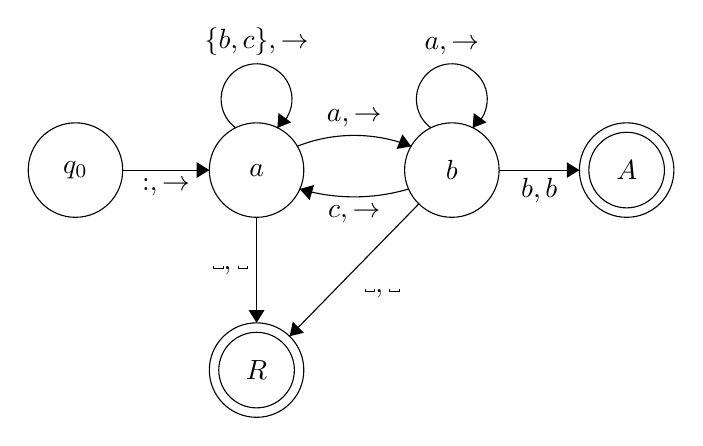
\begin{tikzpicture}[scale=0.2]
\tikzstyle{every node}+=[inner sep=0pt]
\draw [black] (15.4,-24.4) circle (3);
\draw (15.4,-24.4) node {$q_0$};
\draw [black] (26.9,-24.4) circle (3);
\draw (26.9,-24.4) node {$a$};
\draw [black] (39.3,-24.4) circle (3);
\draw (39.3,-24.4) node {$b$};
\draw [black] (50.4,-24.4) circle (3);
\draw (50.4,-24.4) node {$A$};
\draw [black] (50.4,-24.4) circle (2.4);
\draw [black] (26.9,-37.1) circle (3);
\draw (26.9,-37.1) node {$R$};
\draw [black] (26.9,-37.1) circle (2.4);
\draw [black] (18.4,-24.4) -- (23.9,-24.4);
\fill [black] (23.9,-24.4) -- (23.1,-23.9) -- (23.1,-24.9);
\draw (21.15,-24.9) node [below] {$:,\ra$};
\draw [black] (29.478,-22.889) arc (111.61948:68.38052:9.829);
\fill [black] (36.72,-22.89) -- (36.16,-22.13) -- (35.79,-23.06);
\draw (33.1,-21.7) node [above] {$a,\ra$};
\draw [black] (25.577,-21.72) arc (234:-54:2.25);
\draw (26.9,-17.15) node [above] {$\{b,c\},\ra$};
\fill [black] (28.22,-21.72) -- (29.1,-21.37) -- (28.29,-20.78);
\draw [black] (26.9,-27.4) -- (26.9,-34.1);
\fill [black] (26.9,-34.1) -- (27.4,-33.3) -- (26.4,-33.3);
\draw (26.4,-30.75) node [left] {$\tvs,\tvs$};
\draw [black] (37.2,-26.55) -- (29,-34.95);
\fill [black] (29,-34.95) -- (29.91,-34.73) -- (29.2,-34.03);
\draw (33.63,-32.22) node [right] {$\tvs,\tvs$};
\draw [black] (42.3,-24.4) -- (47.4,-24.4);
\fill [black] (47.4,-24.4) -- (46.6,-23.9) -- (46.6,-24.9);
\draw (44.85,-24.9) node [below] {$b,b$};
\draw [black] (37.977,-21.72) arc (234:-54:2.25);
\draw (39.3,-17.15) node [above] {$a,\ra$};
\fill [black] (40.62,-21.72) -- (41.5,-21.37) -- (40.69,-20.78);
\draw [black] (36.558,-25.599) arc (-73.45716:-106.54284:12.146);
\fill [black] (29.64,-25.6) -- (30.27,-26.31) -- (30.55,-25.35);
\draw (33.1,-26.6) node [below] {$c,\ra$};
\end{tikzpicture}
\end{center}

The regular expression is $\cdot ab \cdot$ if we treat the alphabet as implicit, or, if we want to specify the alphabet, we could use $(a|b|c)^\ast ab (a|b|c)^\ast$ .
\end{comment}

\begin{Q}
Let $\Sigma$ be a finite alphabet. Consider the class $\mathcal C$ of Turing machine variants over $\Sigma$ with a countably infinite number of tape heads instead of only one. So the transition function is defined by \begin{equation*}\delta:(Q\setminus H)\times \Sigma^\omega \to Q\times(\Sigma\setminus\{:\}\cup \{\la,\ra\})^\omega \end{equation*}
Let $L\subseteq \Sigma^*$ be any language over $\Sigma$. Show that there is a machine in $\mathcal C$ that decides $L$. What does this tell us about the relative power of $\mathcal C$ and the class of regular Turing machines?

HINT: To make this question easier, you can assume that the machine can tell when different tape heads are reading the same space on the tape, and that this information can be used by the transition function. If you want an extra-difficult challenge try to do without this assumption.
\end{Q}
\begin{comment}
\textbf{Solution}
With the assumption: The machine operates as follows:
\begin{enumerate}
\item Move all the tape heads to the right, so they are all reading the first symbol on the tape.
\item Move all tape heads except the first to the right, so the first is still reading the first symbol, and the rest are reading the second symbol. 
\item Move all except the first and second tape head to the right.
\item Keep following this pattern till the first blank space is found.
\item Now there are $n$ tape heads reading the $n$ characters of the input string, and the rest of the tape heads are all reading a blank space.
\item Write the transition function so that if the string being read is in $L$ the machine accepts, and it rejects otherwise.
\end{enumerate}
The assumption is used here so the machine knows which tape heads to move at each step. E.g. if heads 4 and 5 are reading the same space but heads 3 and 4 are not, it can use this information to say that head 4 must stay in place and all higher numbered heads must move right.
\newline
\newline 
This tells us this new kind of machine is much more powerful than regular Turing machines. 
\newline
\newline
Without the assumption: Let the tape heads be $h_1,h_2,\ldots$. The machine operates as follows:
\begin{itemize}
\item (Step 0) Move all the tape heads to the right, so they are all reading the first symbol on the tape.
\item (Step 1) Move all the tape heads $h_i$ such that $2|i$ to the right, and keep the others in place, except for $h_1$ which moves back to the start of the tape.
\item (Step 2) Move all the tape heads $h_i$ such that $2$ and $3$ divide $i$ to the right. Keep the others in place except $h_1$ which moves back to square 1 (as it must do this), and also move $h_3$ back to the start of the tape.
\item (Step 3) Move all the tape heads $h_i$ such that $i$ is divisible by $2,3,5$ to the right. Keep the others in place except $h_3$ which moves back to square 1, and also move $h_5$ back to the start of the tape.
\item (Step 4) Move the tape heads $h_i$ such that $i$ is divisible by $2,3,5,7$ to the right. Keep the others in place except $h_5$ which moves back to square 1, and also move $h_7$ back to the start of the tape.
\item (Step $k$) To understand the pattern here we list the prime numbers (in order) as $p_1,p_2,\ldots$. At the start of computation step $k>2$, the tape heads with numbers divisible by $p_1\times\ldots \times p_{k-1}$ are reading cell $k-1$. The head $h_{p_{k-1}}$ is also back at the start of the tape reading the $:$ symbol. The fact that $h_{p_{k-1}}$ is reading $:$ is very important, as using this we can code the machine so that it advances all tape heads with numbers divisible by $p_1\times\ldots \times p_{k}$ to the right, and also send head $h_{p_k}$ back ready for the next round.
\item At some point there will be an infinite number of tape heads reading the blank space symbol. This tells the machine the end of the input has been reached.
\item When the end has been reached, we have an infinite set of tape heads reading the first symbol of the input, another infinite set reading the 2nd symbol, and so on. Moreover, these infinite sets are distinguishable by the numbers of the heads they contain (e.g. the first contains odd numbered heads, the second contains those divisible by 2, but not by any other prime, and so on). We write the transition function so that if the string being read is in $L$ the machine accepts, and it rejects otherwise.
\end{itemize}
\end{comment}

The next questions are to revise the concept of countable and uncountable sets, because we'll need them later. You may find it useful to review the class on cardinal numbers from the 531 course.

\begin{Q}
Let $\Sigma$ be a finite alphabet. Prove that $\Sigma^*$ is countably infinite. 
\end{Q}
\begin{comment}
\textbf{Solution}
$\Sigma^*$ is the set of all finite strings using $\Sigma$, so is obviously infinite. To prove it is countable it is sufficient to find a 1-1 function $f:\Sigma^*\to \bbN$. We construct an example of a function like this. Suppose $\Sigma = \{\sigma_1,\ldots,\sigma_n\}$. Let $p_1,p_2,p_3,\ldots$ list the prime numbers in ascending order. Given a string $s = \sigma_{i_1}\sigma_{i_2}\ldots\sigma_{i_k}$, define $f(s) = p_1^{i_1}\times p_2^{i_2}\times \ldots \times p_k^{i_k}$. 

So, for example, if the alphabet is $\{ a = \sigma_0, b = \sigma_1, c=\sigma_2\}$, the string $aacb$ corresponds to $2^13^15^37^2$. I.e., the letter $a$ is at positions 1 and 2 (corresponding to $p_1 = 2$ and $p_2 = 3$, the 1st and 2nd primes), the letter $c$ is at position 3, and the letter $b$ is at position 4. 

Then $f$ is 1-1 because, by the Fundamental Theorem of Arithmetic, numbers are specified uniquely by their prime factorizations (up to reordering).
\end{comment}

\begin{Q}
Let $\Sigma$ again be a finite alphabet. Is $\wp(\Sigma^*)$ countable? Justify your answer.
\end{Q}
\begin{comment}
\textbf{Solution}
This must be uncountable so long as $\Sigma$ is non-empty, because, as proved in the notes for the 531 course, given a non-empty set $X$ we always have $|X|<|\wp(X)|$. 
\end{comment}

\begin{Q}
Recall that the union of a countable number of countable sets is countable. Let $\Sigma=\{0,1\}$ and let $X=\wp(\Sigma^*)$ be the uncountable set of all languages over $\Sigma$. Let $C_1$ and $C_2$ be countable subsets of $X$, and let $U$ be an uncountable subset of $X$. Remember that if $Y$ is a set we use $\bar{Y}$ to denote the complement of $Y$. For each of the following sets say whether it is countable, uncountable, or dependent on the choice of $C_1,C_2,U$. Justify your answers.
\begin{enumerate}[(a)]
\item$C_1\cup C_2$
\item$\bar{C_1}$
\item$\bar{U}$
\item$\bar{C_1}\cap U$
\end{enumerate} 
\end{Q}
\begin{comment}
\textbf{Solution}
\begin{enumerate}[(a)]
\item This is countable as the union of a countable number of countable sets is always countable.
\item This must be uncountable, as $C_1\cup \bar{C}_1 = X$. By part (a), if both $C_1$ and $\bar{C}_1$ were countable then $X$ would be too, but $X$ is uncountable. So, since $C_1$ is countable, $\bar{C}_1$ must be uncountable.
\item This depends on the choice of $U$. If $U = X$ then $\bar{U} = \emptyset$, which is countable. Alternatively, let $U$ be the set of all languages containing the string $s$, for some arbitrary choice of $s$. Then $U$ is in bijection with $\wp(\Sigma^*\setminus\{s\})$, which is uncountable for the same reason $\wp(\Sigma^*)$ is. This bijection takes a language $L\in U$ to $L\setminus\{s\}$, which is in $\wp(\Sigma^*\setminus\{s\})$, and conversely takes $L'\in\wp(\Sigma^*\setminus\{s\})$ to $L'\cup\{s\}$, which is in $U$. Moreover, $\bar{U} = \wp(\Sigma^*\setminus\{s\})$, and so is also uncountable.   
\item This is uncountable, for the following reason.
\begin{align*}
U &= X \cap U \\
&=(\bar{C}_1\cup C_1)\cap U \\
&= (\bar{C}_1 \cap U) \cup (C_1\cap U).
\end{align*}
Now, $(C_1\cap U)$ is countable, so $(\bar{C}_1 \cap U)$ must be uncountable as $U$ is. This last step is essentially the same argument we used in part (b).
\end{enumerate}
\end{comment}



\end{document}
\newpage

\section{Universal Turing Machines}
\documentclass{article}

\usepackage{amsmath, mathrsfs, amssymb, stmaryrd, cancel, relsize,tikz,amsthm}
\usepackage{hyperref}
\theoremstyle{plain}
\newtheorem{theorem}{Theorem}[section]{\bfseries}{\itshape}
\newtheorem{proposition}[theorem]{Proposition}{\bfseries}{\itshape}
\newtheorem{definition}[theorem]{Definition}{\bfseries}{\upshape}
\newtheorem{lemma}[theorem]{Lemma}{\bfseries}{\upshape}
\newtheorem{corollary}[theorem]{Corollary}{\bfseries}{\upshape}
\newtheorem{exercise}[theorem]{Exercise}{\bfseries}{\upshape}

\theoremstyle{definition}
\newtheorem{example}[theorem]{Example}{\bfseries}{\upshape}

\newcommand{\tvs}{\textvisiblespace}
\newcommand{\ra}{\rightarrow}
\newcommand{\la}{\leftarrow}
\newcommand{\co}{\mathbf{code}}


\title{ITCS 532 Foundations of Computer Science\\
Class 3 - Universal Turing Machines}
\author{Rob Egrot}
\date{}

\begin{document}
\maketitle

\subsection{Universal Computation}
Machines for computation have existed for thousands of years. For example, the Antikythera mechanism dates back to the 1st or 2nd century BC, and was used by Ancient Greek astronomers to predict astronomical phenomena such as eclipses. The creation of programs to run on other devices also has a long history. The Banu Musa brothers, for example, invented in 9th century Persia an automatic machine for playing the flute that could be programmed to play different melodies. What distinguishes computers in the modern sense from these early machines is the concept of universal computation. That is, modern computers are able to simulate each other. We could, if we wanted, program a computer to perform the calculations of something like the Antikythera mechanism, or to imitate the Banu Musa brothers' flute player, but we could not, on the other hand, program the mechanical flute player to run Microsoft Windows. 

The first `true' computer (what we will call \emph{universal} computers) is thought to be Charles Babbage's Analytical Engine, designed, with significant contributions from Ada Lovelace, in 1837. This was an entirely mechanical device capable of performing arithmetic calculations and with flow control in the form of conditional branching and looping. This machine was never built due to the significant engineering challenge it posed. For reference, the Difference Engine no. 2, a simpler, non-universal, calculating engine designed by Babbage before the Analytical Engine was over 3 meters long and weighed 2.6 tons when it was finally built in 2002 (see Figure \ref{DE2}). 


\begin{figure}[ht]
\centering
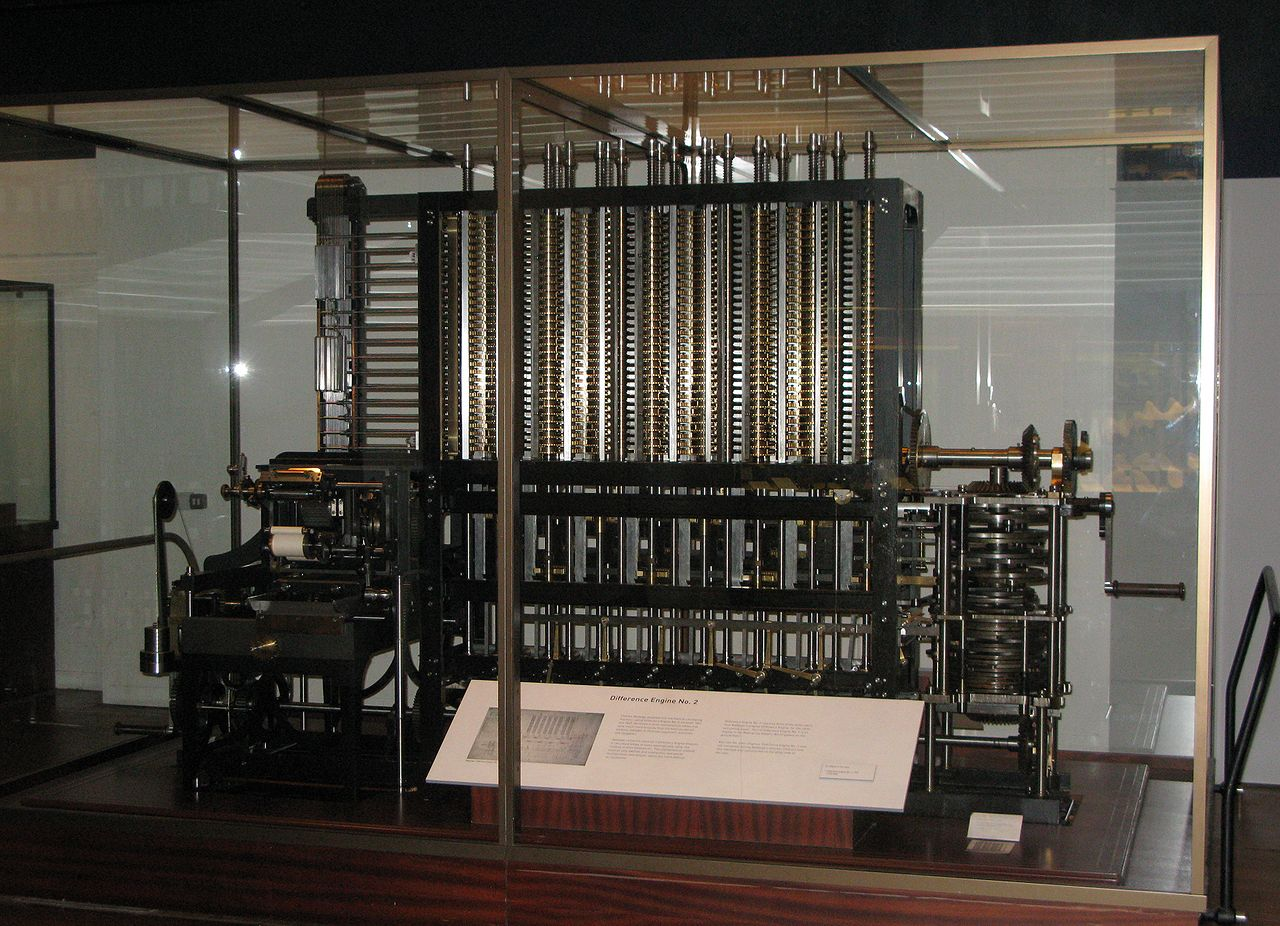
\includegraphics[scale = 0.22]{DE2.jpg}  
\caption{The Difference Engine no. 2. Photo from Wikipedia (https://commons.wikimedia.org/w/index.php?curid=4807331)}
\label{DE2}
\end{figure}

The remarkable thing about the Analytical Engine is that it \emph{could}, in theory, run Windows, though extremely slowly. While Babbage and Lovelace are possibly the first people to design a `modern' computer (in function, if not in form), they did not have the theoretical framework to fully understand what made their idea so revolutionary. The formalism of Turing machines provides this framework for us, and this is what we will explore in this section.  



\subsection{Encoding Turing Machines}
Remember that a Turing machine is defined by a $5$-tuple $(Q,\Sigma,q_0,H,\delta)$. Each part of this is finite. When we've been defining Turing machines we've been defining alphabets and states on an ad hoc basis. For example, we say things like ``let $\Sigma=\{a,b\}$'', or ``let $\Sigma=\{1,*\}$". When we choose an alphabet for a Turing machine the actual symbols we choose aren't important. For example, we could design equivalent machines using $\{a,b\}$ and $\{1,*\}$ as alphabets, by just, for example, assigning $a$ and $1$ the same meaning, and doing the same for $b$ and $*$. What this means is that the important thing about the alphabet a Turing machine works over isn't the symbols themselves, but just the number of distinct symbols. Since every TM uses only a finite number of symbols in its alphabet, if we have a countably infinite pool of symbols, let's say $\hat{\Sigma}=\{\sigma_0,\sigma_1,\sigma_2,\ldots\}$, then every TM is equivalent to one whose alphabet is a finite subset $\{\sigma_0,\ldots,\sigma_n\}$ of symbols from $\hat{\Sigma}$. We will need to include the special symbols $\tvs$ and $:$ in $\hat{\Sigma}$ too, and also the $\la$ and $\ra$ symbols for tape head control.

Similarly, though we gave the states in our machines arbitrary names sometimes, the important thing is just the number of different states and their roles in the computations. So we can fix $\hat{Q}=\{q_0,q_1,q_2,\ldots\}$ and then every TM is equivalent to one whose states are taken from $\hat{Q}$. 

Given a TM defined by $(Q,\Sigma,q_0,H,\delta)$ we can assume $Q$ is a finite subset of $\hat{Q}$, $\Sigma$ is a finite subset of $\hat{\Sigma}$, $q_0$ is just $q_0$ from $\hat{Q}$, and $:$, $\tvs$, $\la$, and $\ra$ are $\sigma_0$, $\sigma_1$, $\sigma_2$, and $\sigma_3$ from $\hat{\Sigma}$ respectively. Since we can now think of every TM as drawing from a fixed, countable pool of symbols, and since every part of the definition of a TM is finite, a Turing machine is specified by a finite subset of $\hat{Q}\cup\hat{\Sigma}$, along with a transition function $\delta$ that is formally a finite subset of $\hat{Q}\times\hat{\Sigma}\times\hat{Q}\times\hat{\Sigma}$. So the set of all Turing machines corresponds to a subset of the set of all finite subsets of a countable set, and so is countable. In other words there is a 1-1 function $\co$  from the set of all Turing machines to $\{0,1\}^*$. There are lots of ways we can define this function, and we give one example below.

\begin{itemize}
\item For $q_n$ we define $\co(q_n)$ to be $n+1$ `1' symbols. So, e.g. $\co(q_2)=111$.
\item For $\sigma_n$ we define $\co(\sigma_n)$ to be $n+1$ `1' symbols. So, e.g. $\co(\sigma_1)=11$. This is the same as the definition for $q_n$, but this isn't a problem because when we build up $\co$ to apply to whole Turing machines, the coded forms of states and symbols will be differentiated by their relative positions.
\item Given a Turing machine $T$ with states $Q=\{q_0,\ldots,q_m\}$ and alphabet $\Sigma=\{\sigma_0,\ldots,\sigma_n\}$ we define the strings 
\begin{equation*}\co(Q)=\co(q_0)0\co(q_1)0\ldots0\co(q_m)0\end{equation*}
and
\begin{equation*}\co(\Sigma)=\co(\sigma_0)0\co(\sigma_1)0\ldots0\co(\sigma_n)0\end{equation*}
\item Let $q_i$ be the accept state of $T$, and let $q_j$ be the reject state (we can safely assume that $T$ has these and only these halt states). The concatenated string $\co(Q)0\co(\Sigma)0\co(q_i)0\co(q_j)0$ encodes the states and alphabet that define $T$, so all that is left is to find a way to encode $\delta$.
\item $\delta$ is formally defined as a set of tuples $(q,\sigma,q',\sigma')$. We can code a tuple $t=(q,\sigma,q',\sigma')$ as 
\begin{equation*}\co(t)=\co(q)0\co(\sigma)0\co(q')0\co(\sigma')0\end{equation*} 
\item If $\delta$ is defined by tuples $t_1,t_2,\ldots,t_k$ we can define 
\begin{equation*}\co(\delta)=\co(t_1)\co(t_2)\ldots \co(t_k)\end{equation*}
\item Combining all this we can encode $T$ with 
\begin{equation*}\co(T)= \co(Q)0\co(\Sigma)0\co(q_i)0\co(q_j)0\co(\delta)\end{equation*}
\item If $I$ is a string defined by $I=\sigma'_1\sigma'_2\ldots\sigma'_l$ (where the $\sigma'$ are symbols from $\hat{\Sigma}$) we can encode $I$ using 
\begin{equation*}\co(I)=\co(\sigma'_1)0\co(\sigma'_2)0\ldots 0\co(\sigma'_l)\end{equation*}
\item We can encode the pair $(T,I)$ representing the Turing machine $T$ and input $I$ using 
\begin{equation*}\co(T,I)=\co(T)00\co(I)\end{equation*}
\end{itemize}   

The general idea is that strings of 1's represent symbols and states, and 0's are used as separators to indicate where the representation of one aspect of the TM ends and the representation of another part begins.

Consider as an example the Turing machine $T$ with alphabet $\Sigma=\{:,\tvs,a,b\}$ that just adds the symbol $a$ to the end of its input.

\begin{center}
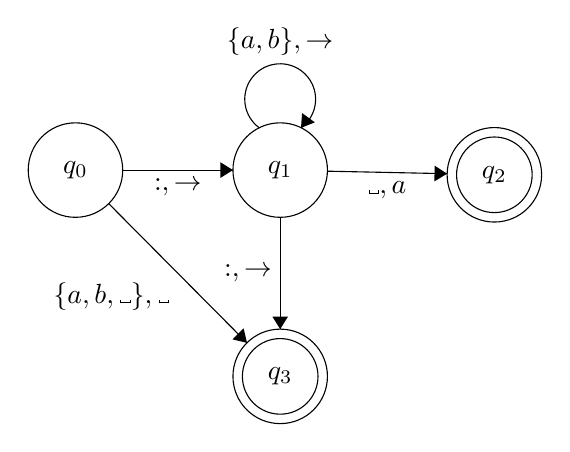
\begin{tikzpicture}[scale=0.2]
\tikzstyle{every node}+=[inner sep=0pt]
\draw [black] (9.4,-31.3) circle (3);
\draw (9.4,-31.3) node {$q_0$};
\draw [black] (22.4,-31.3) circle (3);
\draw (22.4,-31.3) node {$q_1$};
\draw [black] (36,-31.6) circle (3);
\draw (36,-31.6) node {$q_2$};
\draw [black] (36,-31.6) circle (2.4);
\draw [black] (22.4,-44.4) circle (3);
\draw (22.4,-44.4) node {$q_3$};
\draw [black] (22.4,-44.4) circle (2.4);
\draw [black] (12.4,-31.3) -- (19.4,-31.3);
\fill [black] (19.4,-31.3) -- (18.6,-30.8) -- (18.6,-31.8);
\draw (15.9,-31.8) node [below] {$:,\ra$};
\draw [black] (25.4,-31.37) -- (33,-31.53);
\fill [black] (33,-31.53) -- (32.21,-31.02) -- (32.19,-32.02);
\draw (29.17,-32.01) node [below] {$\tvs,a$};
\draw [black] (22.4,-34.3) -- (22.4,-41.4);
\fill [black] (22.4,-41.4) -- (22.9,-40.6) -- (21.9,-40.6);
\draw (21.9,-37.85) node [left] {$:,\ra$};
\draw [black] (11.51,-33.43) -- (20.29,-42.27);
\fill [black] (20.29,-42.27) -- (20.08,-41.35) -- (19.37,-42.05);
\draw (15.38,-39.33) node [left] {$\{a,b,\tvs\},\tvs$};
\draw [black] (21.077,-28.62) arc (234:-54:2.25);
\draw (22.4,-24.05) node [above] {$\{a,b\},\ra$};
\fill [black] (23.72,-28.62) -- (24.6,-28.27) -- (23.79,-27.68);
\end{tikzpicture}
\end{center}

The accept state is $q_2$, and the reject state is $q_3$. To encode this machine we first assign $a$ and $b$ correspondents in $\hat{\Sigma}$. We'll say $a=\sigma_4$ and $b=\sigma_5$ (because $:=\sigma_0$, $\tvs=\sigma_1$, $\la=\sigma_2$, and $\ra=\sigma_3$). The transition function $\delta$ is then defined by the tuples:
\begin{align*}
(q_0,:,q_1,\ra)&=(q_0,\sigma_0,q_1,\sigma_3)\\
(q_0,\tvs,q_3,\tvs)&=(q_0,\sigma_1,q_3,\sigma_1)\\
(q_0,a,q_3,\tvs)&=(q_0,\sigma_4,q_3,\sigma_1)\\
(q_0,b,q_3,\tvs)&=(q_0,\sigma_5,q_3,\sigma_1)\\
(q_1,:,q_3,\ra)&=(q_1,\sigma_0,q_3,\sigma_1)\\
(q_1,a,q_1,\ra)&=(q_1,\sigma_4,q_1,\sigma_3)\\
(q_1,b,q_1,\ra)&=(q_1,\sigma_5,q_1,\sigma_3)\\
(q_1,\tvs,q_2,a)&=(q_1,\sigma_1,q_2,\sigma_4)\\
\end{align*}

So using our definitions we get 
\begin{itemize}
\item $\co(Q)=10110111011110$
\item $\co(\Sigma)=101101110111101111101111110$
\item $\co(q_i)=111$
\item $\co(q_j)=1111$
\item Finally \begin{align*}\co(\delta)=&1010110111101011011110110101111101111011010 \\
                                        &1111110111101101101011110110110111110110111 \\
																				&101101111110110111101101101110111110\end{align*}
\item And so \begin{align*} \co(T)=     &1011011101111001011011101111011111011111100 \\
                                        &1110111101010110111101011011110110101111101\\
																				&1110110101111110111101101101011110110110111\\
																				&110110111101101111110110111101101101110111110                                    																
                                       \end{align*}
\end{itemize}

Because the codes of TMs using this method have a rigid pattern, it's conceptually straightforward to check whether a string is the encoded form of a Turing machine, and it's similarly straightforward to check whether a string is the coded form of a Turing machine along with an input. Specifically, the coded forms of TMs and inputs will follow the pattern \emph{declare states}00\emph{declare symbols}00\emph{declare halt state}0\emph{define transition function}00\emph{input}. Each declaration also has specific syntax which is easily checkable, and of course the declared states, symbols and transition function must all match up properly (e.g. the transition function can't use undeclared states and symbols etc.).

Note that strictly speaking $\co$ isn't a well defined function because it depends on how we write the transition function $\delta$. So the same TM could have different coded forms depending on what order we present the tuples from $\delta$. To solve this problem we can specify an order for writing out the tuples of $\delta$, but we don't need to get into the details of that here. If you check you will see that in the example above the tuples are not listed in alphabetical order. Technically this is a mistake, but we will not worry about this, either here or in the exercises. If we were actually trying to implement a coding system for real, then we'd have to be more careful.  


\subsection{Universal Turing Machines}
Since we can code Turing machines and inputs as finite strings over the alphabet $\{0,1\}$, it is possible to create Turing machines that manipulate these strings. We're interested in a very special kind of Turing machine that can take the coded form of another TM and an input and \emph{simulate} the action of that TM on the input. A Turing machine that can do this with the coded forms of other TMs and their inputs is called \emph{universal}. More precisely, if $U$ is a universal Turing machine (UTM), $T$ is any other TM, and $I$ is an input for $T$, then $U(\co(T,I))$ halts if and only if $T(I)$ halts (and accepts or rejects appropriately), and the output of $U(\co(T,I))$ is the coded form of the output of $T(I)$.

We'll sketch the design of a UTM in a moment, but before that we should realize that universal Turing machines are not strange to us in the 21st century. For example, the computer I wrote these notes on is universal. It can be given coded forms of abstract computation devices (programs) and simulate them on inputs, and this is all universal computation is (although real world universal computers are subject to memory limitations that abstract UTMs are not). The OS of a computer is a program being run over the basic architecture of the system, and the same architecture can support other operating systems too. And the OS itself runs other programs, which may themselves be capable of running other programs, so there are many layers of simulation taking place on a typical home computer.  

Anyway, we now present a rough sketch of how a UTM might work. Our design is for a 3-tape machine to keep things relatively simple. Of course we know that anything we can compute on a 3-tape machine can also be computed on a suitable 1-tape machine.

\begin{itemize}
\item The 1st tape is used for input and output. It starts with $\co(T,I)$ written on it (where $T$ is the machine to be simulated on input $I$). Later in the calculation it will store the state of the tape of $T$ in coded form.
\item The 2nd tape will be used to store $\co(T)$ for reference.
\item The 3rd tape will be used to store the coded form of the state of $T$.
\end{itemize} 

A run of this machine $U$ on input $\co(T,I)$ starts as follows:
\begin{enumerate}
\item $U$ copies $\co(T)$ from tape 1 onto tape 2.
\item $U$ erases $\co(T)$ from tape 1 and shifts $\co(I)$ to the start of the tape so tape 1 just contains $\co(I)$.
\item $U$ writes $\co(q_0)$ on tape 3.
\end{enumerate}

The simulation of a single step of $T(I)$ by $U$ goes as follows:

\begin{enumerate}
\item $U$ searches tape 2 for an instruction corresponding to the state of the machine coded on tape 3 and the symbol currently being read in coded form on tape 1. We need some method for defining which symbol is being read as tape 1 contains the input in coded form. One method we could use is to note that the coded forms of symbols are separated by 0's, so we can define the symbol being read as the one to the left of the 0 being read by the tape head. We just need to manage the tape head on tape one so it ends every simulated step reading a 0.
\item Based on the instruction it updates tape 3 to represent the new state of $T$, and updates tape 1 to represent the new contents of the tape of $T$ and the new position of the tape head.
\item If $T$ has reached a halt state then $U$ halts in the corresponding halt state, otherwise $U$ goes back to 1.
\end{enumerate}


\subsection{Are There Undecidable Problems?}
We claimed in the first class that there are decision problems that cannot be solved by a Turing machine. We will now prove this is true using an abstract argument. In the next class we'll give some specific examples. First remember that every decision problem corresponds to a formal language (a subset of $\Sigma^*$ for some finite alphabet $\Sigma$). Given a finite alphabet $\Sigma$ the set of all finite strings over $\Sigma$, which we call $\Sigma^*$, is countably infinite. The formal languages over $\Sigma$ are the subsets of $\Sigma^*$, so the set of all formal languages over $\Sigma$ is $\wp(\Sigma^*)$, which is uncountable. 

On the other hand, we have just shown that every Turing machine can be represented by a finite string over the alphabet $\{0,1\}$. So the set of all Turing machines (where we count machines that make equivalent computations as being the same) is a subset of the set of all finite strings over $\{0,1\}$, i.e. $\{0,1\}^*$, which is countably infinite. 

So, the set of all Turing machines is countably infinite, but the set of all formal languages over a finite alphabet is uncountably infinite. So there must be (many) more formal languages (and so decision problems) than there are Turing machines capable of deciding them! We conclude that there are decision problems which cannot be decided (or semidecided) by a Turing machine. 

Now, you might first be surprised by this, but after thinking about it for a while you might think that this is to be expected. After all, by identifying formal languages with arbitrary subsets of the set of all finite strings  over the alphabet, we are opening the door for all kinds of strange, undefinable formal languages. So you might be optimistic that, though undecidable problems must exist (by the argument above), at least all the `natural', or `reasonably definable' languages are decidable. But this too is not true, as we shall see in Section \ref{S:und}. 


\subsection{Other Abstract Universal Computers}
It turns out that abstract universal computers are actually very common. Many if not most deterministic processes that are not obviously trivial turn out to be capable of universal computation, in the sense that you can decide rules for input and output that let you simulate Turing machines (including UTMS). 
\newline
\newline
\textbf{Rule 110}\\
An elementary cellular automaton consists of a 2-way infinite tape whose cells can contain either 0 or 1. At each step of a computation the contents of a cell changes based on its contents and the contents of its immediate neighbours. Rule 110 is an elementary cellular automaton with update rules described in the following table.

\begin{center}
\begin{tabular}{| c |c |c |c |c |c |c |c |c|}
\hline
 Cell configuration          & 111 & 110 & 101 & 100 & 011 & 010 & 001 & 000 \\\hline 
 New contents of center cell &  0  &  1  &  1  &  0  &  1  &  1  &  1  &  0\\ \hline   
\end{tabular}
\end{center}

It can be shown that Rule 110 is capable of universal computation. This is a rather vague statement, and it's not clear what it means. In what sense do elementary cellular automata even do `computations' at all? If we wanted to formally prove this assertion, we would have to carefully define concepts like `input', `output' `computation' for cellular automata. Roughly speaking, for a cellular automaton to be `universal' we must be able to define these concepts in such a way that, when the `input' corresponds to the code of a computable function $f$ and a string $I$, the `output' will correspond to the code of $f(I)$. The actual proof that this can be done for Rule 110 is due to Matthew Cook. The proof involves several detours through other forms of computation, and is rather complicated.

Note that Rule 110 can't halt, so we have to adjust the definition of `computation' a bit to take this into account.  
\newline
\newline
\textbf{Conway's Game of Life}\newline
The Game of Life, invented by John Conway, is another example of a cellular automaton, though in this case it is not elementary as it has an infinite grid rather than a single tape. Again each cell contains either 0 or 1. If a cell contains 1 then it is `live' and if it contains 0 then it is `dead'. The update rules are as follows:
\begin{enumerate}
\item A live cell with fewer than two live neighbours dies.
\item A live cell with two or three live neighbours stays live.
\item A live cell with four or more live neighbours dies.
\item A dead cell with exactly three live neighbours becomes live. 
\end{enumerate}

Given how much more complicated this is than Rule 110 it should come as no surprise that the Game of Life is also capable of universal computation, and indeed this is true. Industrious players have created systems for producing many kinds of behaviour within the Game, and you can play around with it at \url{https://bitstorm.org/gameoflife/}.
\newline
\newline
\textbf{Langton's Ant}\\
Langton's ant is essentially a Turing machine variant with an infinite 2D grid instead of a tape. Every square of the grid can be black or white. The `ant' is the tape head. The ant can face in four directions, up, down, left, and right. The movement of the ant is very simple. If the ant is in a white square it turns to the right, colours its square black, then moves forward one square. If the ant is in a black square it turns left, colours its square white, then moves forward one square. Despite its simple behaviour, Langton's ant is also capable of simulating any Turing machine, and so is capable of universal computation (though, like Rule 110 and the Game of Life, there is no way to halt, so we have to adjust the definition of `computation').

Despite the simple deterministic rules, the movements of the ant are often seemingly chaotic (to the human eye) at first, but all known starting configurations of the grid in Langton's ant lead to the ant eventually creating an orderly `highway' out to infinity in one direction. It is an open question whether this is true for all starting configurations. 

You can experiment with this at e.g. \url{https://sciencedemos.org.uk/langton_ant.php}

\end{document}
\subsection{Exercises}
\documentclass{article}

\usepackage{amsmath, mathrsfs, amssymb, stmaryrd, cancel, relsize,tikz,amsthm,comment,graphicx}

\theoremstyle{definition}
\newtheorem{Q}{Question}

\newcommand{\tvs}{\textvisiblespace}
\newcommand{\ra}{\rightarrow}
\newcommand{\la}{\leftarrow}
\newcommand{\co}{\mathbf{code}}

%\includecomment{comment}

% uncomment below to allow file to build as a stand-alone document
% this is part of a hack to allow the same file to be input twice without mixing up labels when building main document
%\renewcommand{\prefix}{}

\title{ITCS 532 Foundations of Computer Science\\
Week 3 - Universal Turing Machines (Homework)}
\author{Rob Egrot}
\date{}

\begin{document}
\maketitle

\begin{Q}\label{\prefix Q:T}
Consider the following Turing machine $T$ over alphabet $\{a\}$.

\begin{center}
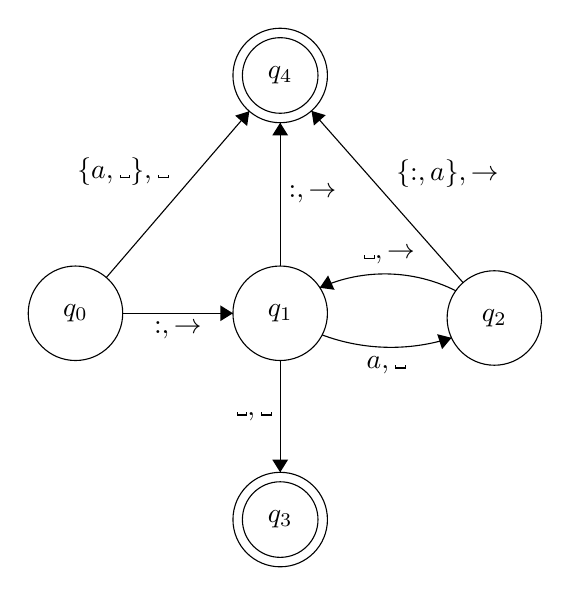
\begin{tikzpicture}[scale=0.2]
\tikzstyle{every node}+=[inner sep=0pt]
\draw [black] (9.4,-31.3) circle (3);
\draw (9.4,-31.3) node {$q_0$};
\draw [black] (22.4,-31.3) circle (3);
\draw (22.4,-31.3) node {$q_1$};
\draw [black] (36,-31.6) circle (3);
\draw (36,-31.6) node {$q_2$};
\draw [black] (22.4,-44.4) circle (3);
\draw (22.4,-44.4) node {$q_3$};
\draw [black] (22.4,-44.4) circle (2.4);
\draw [black] (22.4,-16.2) circle (3);
\draw (22.4,-16.2) node {$q_4$};
\draw [black] (22.4,-16.2) circle (2.4);
\draw [black] (12.4,-31.3) -- (19.4,-31.3);
\fill [black] (19.4,-31.3) -- (18.6,-30.8) -- (18.6,-31.8);
\draw (15.9,-31.8) node [below] {$:,\ra$};
\draw [black] (11.36,-29.03) -- (20.44,-18.47);
\fill [black] (20.44,-18.47) -- (19.54,-18.75) -- (20.3,-19.41);
\draw (15.35,-22.3) node [left] {$\{a,\tvs\},\tvs$};
\draw [black] (33.284,-32.856) arc (-72.05443:-110.47292:12.503);
\fill [black] (33.28,-32.86) -- (32.37,-32.63) -- (32.68,-33.58);
\draw (29.13,-34.02) node [below] {$a,\tvs$};
\draw [black] (24.914,-29.684) arc (114.19527:63.27739:10.059);
\fill [black] (24.91,-29.68) -- (25.85,-29.81) -- (25.44,-28.9);
\draw (29.29,-28.23) node [above] {$\tvs,\ra$};
\draw [black] (22.4,-34.3) -- (22.4,-41.4);
\fill [black] (22.4,-41.4) -- (22.9,-40.6) -- (21.9,-40.6);
\draw (21.9,-37.85) node [left] {$\tvs,\tvs$};
\draw [black] (34.01,-29.35) -- (24.39,-18.45);
\fill [black] (24.39,-18.45) -- (24.54,-19.38) -- (25.29,-18.72);
\draw (29.74,-22.45) node [right] {$\{:,a\},\ra$};
\draw [black] (22.4,-28.3) -- (22.4,-19.2);
\fill [black] (22.4,-19.2) -- (21.9,-20) -- (22.9,-20);
\draw (22.9,-23.75) node [right] {$:,\ra$};
\end{tikzpicture}
\end{center}

What does $T$ do? 

\end{Q}
\begin{comment}
\textbf{Solution}
$T$ erases its input.
\end{comment}

\begin{Q}\label{\prefix Q:delta}
Write out the transition function $\delta$ for $T$ from question \ref{Q:T} in terms of tuples (i.e. $(q,\sigma,q',\sigma'))$.
\end{Q}
\begin{comment}
\textbf{Solution}
\begin{itemize}
\item $(q_0, :, q_1, \ra) = (q_0,\sigma_0,q_1,\sigma_3)$.
\item $(q_0, \tvs, q_4, \tvs) = (q_0,\sigma_1,q_4,\sigma_1)$.
\item $(q_0,a,q_4,\tvs) = (q_0, \sigma_4,q_4,\sigma_1)$.
\item $(q_1, :, q_4, \ra)= (q_1,\sigma_0,q_4,\sigma_3)$.
\item $(q_1,\tvs,q_3,\tvs) = (q_1,\sigma_1,q_3,\sigma_1)$.
\item $(q_1,a,q_2,\tvs) = (q_1,\sigma_4,q_2,\sigma_1)$.
\item $(q_2,:,q_4,\ra) = (q_2,\sigma_0,q_4,\sigma_3)$.
\item $(q_2,\tvs,q_1,\ra) = (q_2,\sigma_1,q_1,\sigma_3)$.
\item $(q_2,a,q_4,\ra) = (q_2,\sigma_4, q_4,\sigma_3)$.
\end{itemize}
\end{comment}

\begin{Q}
Let $T$ be as in question \ref{Q:T}. Using the encoding system from the notes we map every symbol from the alphabet of $T$ to some symbol in $\{\sigma_0,\sigma_1,\ldots\}$. Since $\sigma_0$, $\sigma_1$, $\sigma_2$, and $\sigma_3$ are taken by $:$, $\tvs$, $\la$ and $\ra$ respectively we let $a=\sigma_4$. Using the system from the notes and your transition function from question \ref{Q:delta} write down $\co(T)$.
\end{Q}
\begin{comment}
\textbf{Solution}\\
Assuming tuples in the same order as in the solution above (which is essentially arbitrary - if we were designing a real encoding scheme we would want to use something more principled than this):\\
 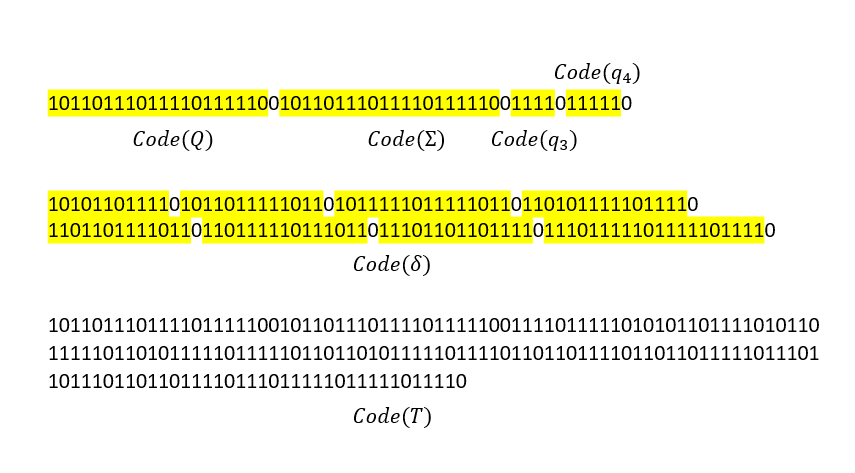
\includegraphics[width=\linewidth]{code.png}
\end{comment}

\begin{Q}
Suppose $T$ is a Turing machine over the alphabet $\{0,1,*\}$ that takes as input two binary numbers separated by $*$ and outputs their sum (in binary). Describe a way we could use $T$ to construct a Turing machine that takes as input two positive binary numbers separated by $*$ and outputs their product. You can use multiple tapes. You don't need to draw a state change diagram.
\end{Q}
\begin{comment}
\textbf{Solution}\\
\begin{enumerate}
\item Copy first number to tape 2.
\item Copy second number to tape 3. 
\item Trim tape 1 so it just contains first number.
\item If tape 3 is empty then erase tape 1 and halt.
\item If the number on tape 3 is one then halt.
\item Add number on tape 2 to the number on tape 1, then decrease number on tape 3 by one (we use $T$ in this step).
\item Go to step 5).
\end{enumerate}

We can assume we have an extra tape for side calculations if we like. We could also check to see if the first number is zero before step 6. Otherwise the machine may add zero to itself several times. This will get the right answer, but is obviously inefficient. 
\end{comment}



\end{document}
\newpage

\section{Undecidable Problems}\label{S:und}
\documentclass{article}

\usepackage{amsmath, mathrsfs, amssymb, stmaryrd, cancel, relsize,tikz,amsthm}
\theoremstyle{plain}
\newtheorem{theorem}{Theorem}[section]{\bfseries}{\itshape}
\newtheorem{proposition}[theorem]{Proposition}{\bfseries}{\itshape}
\newtheorem{definition}[theorem]{Definition}{\bfseries}{\upshape}
\newtheorem{lemma}[theorem]{Lemma}{\bfseries}{\upshape}
\newtheorem{corollary}[theorem]{Corollary}{\bfseries}{\upshape}
\newtheorem{exercise}[theorem]{Exercise}{\bfseries}{\upshape}

\theoremstyle{definition}
\newtheorem{example}[theorem]{Example}{\bfseries}{\upshape}

\newcommand{\tvs}{\textvisiblespace}
\newcommand{\ra}{\rightarrow}
\newcommand{\la}{\leftarrow}
\newcommand{\co}{\mathbf{code}}

\title{ITCS 532 Foundations of Computer Science\\
Class 4 - Undecidable Problems}
\author{Rob Egrot}
\date{}

\begin{document}
\maketitle
\subsection{The Halting Problem}
Given a Turing machine $T$ and an input $I$, either $T(I)$ halts or it runs forever. One must happen, and both cannot be true at the same time. So the question of whether a Turing machine $T$ halts on input $I$ is a \emph{decision problem} whose instances are pairs $(T,I)$. 

Moreover, we know that we can encode pairs $(T,I)$ of Turing machines and inputs over the alphabet $\{0,1\}$. So, the question is, can we create a Turing machine that decides this problem? In other words, is there a TM that takes as input $\co(T,I)$ and accepts if $T(I)$ halts, and rejects if it does not (or if its input is not the code for a TM and an input)? 

This is an important question, so it needs thinking about. If a Turing machine $H$ exists that can decide the halting problem then, for one thing, it would imply that r.e. languages are recursive (see Exercise \ref{E:H}). So suppose $H$ exists. In other words, suppose for any input $J$ we have $H(J)$ accepts if $J=\co(T,I)$ for some Turing machine $T$ and input $I$ such that $T(I)$ halts, and rejects otherwise. What are the consequences of this? Does it lead to a contradiction? 

In mathematics and logic there are many paradoxes associated with self reference (e.g. Russell's paradox, the barber paradox). A good `stress test' for $H$ is how it handles references to itself. But how would $H$ reference itself? Well, since we can encode Turing machines as strings it formally makes sense to run a TM on the encoded version of itself. I.e. given a Turing machine $T$ we can run $T$ on $\co(T)$. 

Since it makes sense to run $T$ on $\co(T)$, it also makes sense to ask whether $T(\co(T))$ halts. Since we are assuming we have a machine $H$ for solving the halting problem, we can modify $H$ to find a machine that solves the problem ``Given $T$, does $T(\co(T))$ halt?". We'll call this machine $H'$. The operation of $H'$ is straightforward; it takes input $\co(T)$ then simulates $H$ on input $\co(T,\co(T))$. It accepts if $H$ accepts, and rejects otherwise. If we run $H'$ on something that is not the code of a Turing machine, then we can assume it rejects, as using a coding scheme such as the one from the last section, whether or not a string is the code of a Turing machine is decidable. 

At this point we might try running $H'$ on itself. In other words, we might investigate $H'(\co(H'))$. Is it possible that $H'(\co(H'))$ runs forever? No, because $H'(\co(H'))$ works internally by running $H(\co(H',\co(H')))$, and as we are assuming that $H$ decides the halting problem, this computation must halt. Is it possible that $H'(\co(H'))$ rejects? Again no, but this time for a slightly different reason. If $H'(\co(H'))$ rejects then that means $H(\co(H',\co(H')))$ rejects, but as $H$ is supposed to decide the halting problem, this would mean that $H'(\co(H'))$ does not halt, which would be a contradiction. Can $H'(\co(H'))$ accept? This time the answer is yes, because this means $H(\co(H',\co(H')))$ accepts, which does not lead to a contradiction. So, we cannot rule out the possibility of the existence of $H$ just by constructing $H'$ and running $H'(\co(H'))$.

The idea now is to modify $H'$ slightly to close the `escape route' of acceptance described above. We define a new machine $H''$. This machine is based on $H'$ but it halts if the input machine \emph{doesn't} halt on the coded form of itself, and it loops forever if the input machine halts on the coded form of itself. This modification is easy to make; it's similar to the one we used to prove that recursive languages are recursively enumerable. 
\[H''(\co(T))=\begin{cases}Halt \text{ if } T(\co(T)) \text{ doesn't halt}\\ Loop\text{ }forever \text{ if } T(\co(T)) \text{ halts}\end{cases}\]
In addition, $H''(I)$ halts if $I$ is not the coded form of a TM.

Now think about what happens when we run $H''$ on its own code. I.e. what is $H''(\co(H''))$? Well, according to the definition, $H''(\co(H''))$ halts if and only if $H''(\co(H''))$ doesn't halt. This is a clear contradiction, so we must conclude that $H''$ cannot exist. But $H''$ is a simple modification of $H$, so $H$ cannot exist either. This gives us:

\begin{theorem}
The halting problem is undecidable.
\end{theorem}
 
Moreover, it's easy to show the halting problem is semidecidable, so we also get:

\begin{corollary}
The set of recursive languages is strictly contained in the set of r.e. languages.
\end{corollary}

\begin{exercise}\label{E:H}
Why would the existence of a TM for solving the halting problem imply that r.e. languages are recursive?\footnote{This is maybe not so obvious. The idea is that, given a Turing machine $T$ that semidecides a language $L$, if you also had a machine that decided the halting problem then you could design a machine $T'$ that decides $L$. Explicitly, given and input $I$, the machine $T'$ would simulate $H(\co(T,I))$. If this accepts then $T(I)$ halts, and so $I\in L$. On the other hand, if it rejects then $T(I)$ does not halt, and so $I\notin L$. So the machine $T'$ decides $L$ as claimed. }
\end{exercise}  

\begin{exercise}
Why is the halting problem semidecidable?
\end{exercise}



\subsection{Languages That Are Not R.E.}
The halting problem is semidecidable but not decidable, so its associated language is r.e. but not recursive. We know from the countable vs uncountable argument that there are languages that are not r.e., but can we find a specific example? It turns out the answer is yes, and one way we can do this is to use the halting problem. First we present some useful facts about recursive and r.e. languages.

\begin{theorem}\label{T:rec}
If $L$ is a recursive formal language then the complement language $\bar{L}$ is also recursive.
\end{theorem}
\begin{proof}
If $L$ is recursive then there's a Turing machine $T$ that accepts if $I\in L$ and rejects if $I\notin L$. To get a machine that decides $\bar{L}$ we just need to swap the `accept' and `reject' states of $T$.
\end{proof}

\begin{theorem}\label{T:comps}
Let $L$ be a formal language over a finite alphabet. If $L$ is r.e. and the complement language $\bar{L}$ is also r.e. then $L$ is recursive.
\end{theorem}
\begin{proof}
If there are machines $T_1$ and $T_2$ that semidecide $L$ and $\bar{L}$ respectively then we can construct a machine $T$ to decide $L$ as follows. Given input $I$ we simulate $T_1(I)$ and $T_2(I)$. Either $I\in L$ or $I\in \bar{L}$ so one of $T_1(I)$ and $T_2(I)$ will halt. If $T_1(I)$ halts $T$ accepts, if $T_2(I)$ halts then $T$ rejects.  
\end{proof}

\begin{theorem}
Let $L_1$ and $L_2$ be formal languages over a finite alphabet.
\begin{enumerate}
\item If $L_1$ and $L_2$ are recursive then $L_1\cup L_2$ and $L_1\cap L_2$ are recursive.
\item If $L_1$ and $L_2$ are r.e. then $L_1\cup L_2$ and $L_1\cap L_2$ are r.e.
\end{enumerate}
\end{theorem}
\begin{proof}
If $T_1$ and $T_2$ are machines that decide $L_1$ and $L_2$ respectively, then we can construct a machine $T$ that decides $L_1\cup L_2$ or $L_1\cap L_2$ by simulating $T_1$ and $T_2$ on any input $I$. If either $T_1(I)$ or $T_2(I)$ accepts then $I\in L_1\cup L_2$. On the other hand, if both reject then $I\notin L_1\cup L_2$. Similarly, if both accept then $I\in L_1\cap L_2$, but if one rejects then $I\notin L_1\cap L_2$.

Finally, if $T_1$ and $T_2$ are machines that semidecide $L_1$ and $L_2$ then $I\in L_1\cup L_2$ if and only if either $T_1(I)$ or $T_2(I)$ halts, and $I\in L_1\cap L_2$ if and only if $T_1(I)$ and $T_2(I)$ both halt. 
\end{proof}

Now we have covered the background material consider the following languages.

\begin{definition}[$SA$ - `self accepting']\label{D:SA}
$SA$ is the language over $\{0,1\}$ that contains the codes of all Turing machines $T$ such that $T(\co(T))$ halts. In other words $SA$ contains all yes instances of the modified halting problem `solved' by $H'$ in the previous section.
\end{definition}

\begin{definition}[$NSA$ - `not self accepting']\label{D:NSA}
$NSA$ is the language over $\{0,1\}$ that contains the codes of all Turing machines $T$ such that $T(\co(T))$ does not halt.
\end{definition}

\begin{definition}[$NSA'$]
$NSA'$ is $NSA$ together with all the strings that are not codes for Turing machines. So $NSA'=\overline{SA}$.
\end{definition}


Since the modified halting problem is semidecidable but not decidable we know that $SA$ is r.e. but not recursive. This gives us the following result.

\begin{theorem}
$NSA'$ is not r.e.
\end{theorem}
\begin{proof}
Since $SA$ is r.e., if $NSA'$ is also r.e. then $SA$ is recursive by theorem \ref{T:comps} (as $NSA'=\overline{SA}$). But $SA$ is not recursive, so $NSA'$ cannot be r.e.
\end{proof}

\begin{corollary}
$NSA$ is not r.e.
\end{corollary}
\begin{proof}
By the definition of coding there is an algorithm that says whether a string $x$ is or is not the coded form of a Turing machine. So if $NSA$ was r.e. then we could combine the algorithm semideciding $NSA$ with the algorithm deciding which strings are codes for Turing machines like this:
\begin{enumerate}
\item Check if input string $x$ is the code of a Turing machine. If no then halt, if yes go to step 2.
\item Run algorithm semideciding $NSA$. If this halts then halt, otherwise just keep going. 
\end{enumerate} 
This algorithm semidecides $NSA'$, which is a contradiction because we know $NSA'$ is not r.e.
\end{proof}

We could also prove that $NSA$ is not r.e. directly, using similar logic to what we used to show the halting problem is not decidable.

\begin{theorem}\label{T:NSAalt}
$NSA$ is not r.e. (without using the fact that the modified halting problem is undecidable).
\end{theorem}
\begin{proof}
Suppose there is a machine $M$ that semidecides $NSA$. So $M(\co(T))$ halts if $T(\co(T))$ does not halt, and runs forever if $T(\co(T))$ halts. So by definition $M(\co(M))$ halts if and only if $M(\co(M))$ does not halt, which is a contradiction.
\end{proof}

\begin{corollary}\label{C:NSA'}
$NSA'$ is not r.e.
\end{corollary}
\begin{proof}
If $NSA'$ were r.e. then we could use the following algorithm on input string $x$:
\begin{enumerate}
\item Run the algorithm that semidecides $NSA'$. If this halts then go to the next step.
\item Run the algorithm that decides if $x$ is the code of a Turing machine. If $x$ is the code of a Turing machine then it must not be self-accepting, as it's in $NSA'$. This means it's in $NSA$, so we should halt. If $x$ is not the code of a Turing machine then we should instead go into an infinite loop.   
\end{enumerate}
This algorithm semidecides $NSA$, which would contradict the fact that $NSA$ is not r.e. 
\end{proof}

We can also use previously proved results to show that $SA$ is not recursive without referencing the halting problem.
\begin{theorem}
$SA$ is not recursive.
\end{theorem}
\begin{proof}
If $SA$ is recursive then $\overline{SA}=NSA'$ is recursive by theorem \ref{T:rec}. This would contradict corollary \ref{C:NSA'}.
\end{proof}

The circle of proofs we've just gone through produces two conceptually straightforward languages (and thus decision problems), one of which is recursive but not r.e. ($SA$), and the other which is not even r.e. ($NSA$). The arguments are perhaps easier to understand than the somewhat complicated definition of $H''$ used in the proof that the halting problem is not recursive. In particular the proof that $NSA$ is not r.e. from theorem \ref{T:NSAalt} uses self-reference to get a contradiction in a much more direct way than the proof that the halting problem is undecidable does. However, the halting problem is independently interesting, and historically important, which is why we discuss it in some detail and don't just take the easy route to find our non-recursive and non-r.e. languages. 


\subsection{Reduction}
We know that the halting problem is undecidable. That is, there is no Turing machine $H$ that can act on $\co(T,I)$ for another Turing machine $T$ and accept if $T(I)$ halts and reject if it does not. Consider the following decision problem.

\begin{definition}[empty tape halting problem]
Is there a Turing machine $E$ that given $\co(T)$ for another Turing machine $T$ will accept if $T$ halts on the empty string and will reject otherwise?
\end{definition}

Suppose this machine $E$ exists. Consider a Turing machine $T$ and an input $I$. Using $T$ and $I$ we design a new Turing machine $T_I$ that does the following on input $J$.
\begin{enumerate}
\item $T_I$ erases input $J$ from the tape.
\item $T_I$ simulates $T$ on $I$.
\end{enumerate}

What happens if we run $E$ on $\co(T_I)$?
\begin{itemize}
\item $E(\co(T_I))$ accepts $\iff T_I$ halts on empty input $\iff T(I)$ halts.
\item $E(\co(T_I))$ rejects $\iff T_I$ does not halt on empty input $\iff T(I)$ does not halt.
\end{itemize}

This looks a lot like solving the halting problem, which we know is impossible. We can formalize this intuition by using $E$, assuming it exists, to construct a machine $H$ for solving the halting problem. This can't happen so we will conclude that $E$ cannot exist. Assuming, for the sake of our argument, that $E$ \emph{does} exist we construct $H$ as follows.

\begin{enumerate}
\item Given input $\co(T,I)$ the first thing $H$ does is construct $\co(T_I)$. This is complicated but it can be done.
\item $H$ then simulates $E(\co(T_I))$.
\item $H(\co(T,I))$ accepts $\iff E(\co(T_I))$ accepts $\iff T(I)$ halts, and rejects otherwise. 
\end{enumerate}

$H$ is a well defined Turing machine, and $H$ solves the halting problem. The only questionable step in the construction of $H$ is the assumption that $E$ exists. Since $H$ cannot exist we conclude that $E$ cannot exist either, and so the empty tape halting problem is also undecidable.

This is an example of a general technique called \emph{reduction}. The general strategy is as follows.

\begin{enumerate}
\item Start with a decision problem $D$ whose decidability is not known, and a decision problem $U$ that is known to be undecidable (e.g. the halting problem).
\item Show that instances $I_U$ of $U$ can be converted by an algorithm to instances $I_D$ of $D$ so that
\begin{itemize}
\item $I_D$ is a yes instance of $D\iff I_U$ is a yes instance of $U$.
\item $I_D$ is a no instance of $D\iff I_U$ is a no instance of $U$.
\end{itemize}
\item If there is an algorithm for solving $D$ then we could combine this with our instance converting algorithm to find an algorithm for solving $U$.
\item Since $U$ is undecidable no algorithm for solving $U$ exists, and we conclude that an algorithm for solving $D$ cannot exist either.
\end{enumerate} 

More generally, given decision problems $A$ and $B$ we say: 

\begin{definition}[reducible]
\emph{$A$ is reducible to $B$} if there is an algorithm that converts instances $I_A$ of $A$ to instances $I_B$ of $B$ so that $I_B$ is a yes instance of $B$ if and only if $I_A$ is a yes instance of $A$, and $I_B$ is a no instance of $B$ if and only if $I_A$ is a no instance of $A$.\end{definition}

\begin{definition}[$A\leq B$]
Given decision problems $A$ and $B$ we write $A\leq B$ if $A$ is reducible to $B$. Informally we think of this as meaning that $B$ is at least as hard as $A$. The justification for this is that if we had a solution for $B$ we could use it to solve $A$, but we wouldn't necessarily be able to use a solution for $A$ to solve $B$. In the example above we would write $U\leq D$.
\end{definition} 

  

This produces a kind of hierarchy of problems (and formal languages), ordered by their relative decidability. It turns out that, so long as we ignore `decision problems' with only yes, or only no, instances, all the decidable problems are grouped together at the bottom of this hierarchy. This is due to the following result.  
\begin{theorem}
Let $D$ be a decidable problem, and let $A$ be any other decision problem with at least one yes instance and at least one no instance. Then $D\leq A$.
\end{theorem}
\begin{proof}
We want an algorithm that takes an instance $I_D$ of $D$ and converts it to an instance $I_A$ of $A$ so that $I_D$ is `yes' if and only if $I_A$ is `yes', and $I_D$ is `no' if and only if $I_A$ is `no'. Since $D$ is decidable, given an instance $I_D$ of $D$ we can find out whether it is `yes' or `no' by running the decision algorithm for $D$. If $I_D$ is a `yes' we convert it to a `yes' of $A$, and if not we convert it to a `no' of $A$. 
\end{proof}

\begin{exercise}
Show that for decision problems the $\leq$ relation is reflexive (i.e. $A\leq A$), and transitive (i.e. $A\leq B$ and $B\leq C\implies A\leq C$).
\end{exercise}

\begin{exercise}
Show that $\leq$ is not symmetric.
\end{exercise}

As mentioned above, there is a hierarchy of decision problems, with all the decidable ones at the bottom. You might think that this hierarchy is very simple, with the decidable problems all grouped together at the bottom, and all the undecidable ones grouped together at the top. But it turns out this doesn't happen, because some problems are more undecidable than others. We will not go into the details of this here, but the idea is you imagine equipping Turing machines with an \emph{oracle} that, for example, magically solves the halting problem. If you have a machine with an oracle for solving the halting problem, then you can, obviously, solve the halting problem, but it turns out there are other problems that you still cannot solve. So you can imagine adding an oracle for solving one of these `next level' undecidable problems, and again it turns out there are problems you still cannot solve. This leads to the concept of \emph{Turing degrees}. We will not explore this, but the basic fact is that the reducibility hierarchy is actually uncountably infinite and extremely complicated.  

\subsection{More Reductions}
Here are some more decision problems whose undecidability we can prove using reduction.\newline\newline
\textbf{Halts for all Inputs ($HAI$)}\newline 
Suppose we have the code of a Turing machine $T$. Is there an algorithm that we can run on $\co(T)$ that tells us whether or not $T(I)$ halts for all inputs $I$? The answer is no, and one of the exercises for this section is to prove this by reducing the halting problem to this problem (i.e. to show that $HP\leq HAI$).\newline\newline
\textbf{Equivalence of Turing machines ($ETM$)}\newline
Suppose we have the code for two Turing machines. Is there an algorithm we can use that will tell us if they do the same thing for all inputs (i.e. if $T_1(I)=T_2(I)$ for all $I$)? It turns out the answer is no, and we can prove this using the reduction technique. The idea is to show that the `halts for all inputs' problem' is reducible to the `equivalence of Turing machines' problem (i.e. that $HAI\leq ETM$).

An instance of $HAI$ is just a Turing machine $T$, and $T$ is a yes instance if and only if $T(I)$ halts for all $I$. As mentioned above, one of the exercises for this chapter is to show that $HAI$ is undecidable. We want to use $T$ to algorithmically construct $T_1$ and $T_2$ so that $T(I)$ halts for all $I$ if and only if $T_1(I)=T_2(I)$ for all $I$. 

We construct $T_1$ so that it operates as follows:
\begin{enumerate}
\item $T_1(I)$ simulates $T(I)$.
\item If $T(I)$ halts then $T_1(I)$ erases the tape then writes a single `1' before halting. 
\end{enumerate} 

We construct $T_2$ so that $T_2(I)$ just writes a single `1' on the tape before halting for all $I$.

Now, $T$ is a yes instance of $HAI$ if and only if $T(I)$ halts for all $I$, and this happens if and only if $T_1(I)$ writes a single `1' for all $I$. But $T_1(I)=1$ for all $I$ if and only if $T_1(I)=T_2(I)$ for all $I$. So $T$ is a `yes' instance of $HAI$ if and only if $(T_1,T_2)$ is a yes instance of $ETM$. So $HAI\leq ETM$ and since $HAI$ is undecidable we deduce that $ETM$ is undecidable too.
\newline
\newline
\textbf{Does $T$ write $\sigma$?}\newline
Consider the following decision problem. Given a Turing machine $T$ and a symbol $\sigma$ in the alphabet of $T$, does $T$ write $\sigma$ on the tape when started with an empty tape? We can prove that this is undecidable by reducing the empty tape halting problem ($ETHP$) to it. For convenience we'll call the problem we're looking at here $D$. Given an instance $T$ of $ETHP$ we construct an instance $(T',\sigma)$ of $D$ as follows:
\begin{enumerate}
\item We choose $\sigma$ to be any symbol not appearing in the alphabet of $T$.
\item We construct $T'$ so that it operates as follows:
\begin{enumerate}
\item $T'(I)$ checks if $I=\epsilon$ and halts if it is not.
\item $T'(\epsilon)$ simulates $T(\epsilon)$ (without using the symbol $\sigma$), except that if $T(\epsilon)$ halts then $T'(\epsilon)$ writes $\sigma$ and then halts. 
\end{enumerate}
\end{enumerate}
So $T$ is a yes instance of $ETHP$ if and only if $T'$ writes $\sigma$ on the tape when run on $\epsilon$. I.e. $T$ is a yes instance of $ETHP$ if and only if $(T',\sigma)$ is a yes instance of $D$. So $ETHP\leq D$ and we deduce that $D$ is undecidable.


\end{document}
\subsection{Exercises}
\documentclass{article}

\usepackage{amsmath, mathrsfs, amssymb, stmaryrd, cancel, relsize,tikz,amsthm,comment,enumerate}

\theoremstyle{definition}
\newtheorem{Q}{Question}

\newcommand{\tvs}{\textvisiblespace}
\newcommand{\ra}{\rightarrow}
\newcommand{\la}{\leftarrow}
\newcommand{\co}{\mathbf{code}}


\title{ITCS 532 Foundations of Computer Science\\
Week 4 - Undecidable Problems (Homework)}
\author{Rob Egrot}
\date{}
%\includecomment{comment}

% uncomment below to allow file to build as a stand-alone document
% this is part of a hack to allow the same file to be input twice without mixing up labels when building main document
%\renewcommand{\prefix}{}

\begin{document}
\maketitle

\begin{Q}
Let $L_1$ and $L_2$ be disjoint r.e. languages. Suppose $L_1\cup L_2$ is recursive. Prove that $L_1$ and $L_2$ are both recursive.
\end{Q}
\begin{comment}
\textbf{Solution}\\
We will describe an algorithm for deciding $L_1$. 
\begin{enumerate}
\item Given a string $x$ we can decide if $x\in L_1\cup L_2$, as this language is recursive.
\item If $x\notin L_1\cup L_2$ then $x\notin L_1$, so reject.
\item If $x\in L_1\cup L_2$ then it must be in either $L_1\setminus L_2$, or $L_2\setminus L_1$. Use dovetailing to simultaneously run the algorithms that semidecide $L_1$ and $L_2$ on $x$.
\item If $x\in L_1$ then accept.
\item If $x\in L_2$ then reject.
\end{enumerate}
We can decide $L_2$ similarly.
\end{comment}

\begin{Q}\label{\prefix Q:100}
Let $D$ be the decision problem ``Given a Turing machine $T$ and input $I$, does $T(I)$ halt within 100 steps?". Then there is an associated formal language \[L_D=\{\co(T,I):T \text{ halts on } I \text{ within 100 steps}\}\]
Which of the following is true (give reasons)?
\begin{enumerate}
\item[i)] $L_D$ is recursive.
\item[ii)] $L_D$ is r.e but not recursive.
\item[iii)] $L_D$ is not r.e.
\end{enumerate}
\end{Q}
\begin{comment}
\textbf{Solution}\\
$L_D$ is recursive. To decide $L_D$ we use a Turing machine that, given input $\co(T,I)$ simulates $T(I)$, and also maintains a counter track of the number of steps that have been simulated. If this simulation halts before the counter reaches 100 then the input is accepted. If it does not (or if the input is not in the correct format), then it rejects.
\end{comment}

\begin{Q}\label{\prefix Q:D}
Let $D$ be the decision problem ``Given a Turing machine $T$, does $T$ halt on every input $I$ within 100 steps?". What is the formal language $L_D$ associated with $D$?
\end{Q}
\begin{comment}
\textbf{Solution}\\
$\{\co(T): T$ is a Turing machine and $T(I)$ halts within 100 steps for all $I\}$.
\end{comment}

\begin{Q}
With $D$ as in question \ref{Q:D} prove that $L_D$ is recursive. 
\end{Q}
\begin{comment}
\textbf{Solution}\\
Note that $T(I)$ halts for all $I$ within 100 steps if and only if $T(I)$ halts for all $I$ of length $\leq 100$ within 100 steps, as $T$ can never read past the first 100 symbols within 100 steps. Now, the number of strings over a finite alphabet whose length is $\leq 100$ is finite, so we can check $T(I)$ for each such string $I$ using the algorithm from question \ref{Q:100}. If the answer is no for any $I$ we reject $\co(T)$, and if the answer is yes for all $I$ we accept $\co(T)$.
\end{comment}

\begin{Q}
Let $HAI$ be the decision problem ``Given $T$ does $T$ halt for all inputs?". Then an instance of $HAI$ is a Turing machine $T$. \begin{enumerate}
\item[a)] What is an instance of the Halting Problem?
\item[b)] If $M$ is a Turing machine and $I$ is an input for $M$ let $M_I$ be a machine that first erases its input then simulates $M(I)$. Show that $M(I)$ halts if and only if $M_I(J)$ halts for all inputs $J$, and $M(I)$ runs forever if and only if $M_I(J)$ runs forever for all $J$.
\item[c)] Prove that the Halting Problem reduces to $HAI$.
\item[d)] What does this tell us about the decidability of $HAI$?
\end{enumerate} 
\end{Q}
\begin{comment}
\textbf{Solution}\\
\begin{enumerate}[a)]
\item A pair $(M,I)$ where $M$ is a Turing machine and $I$ is a finite string over its alphabet.
\item By definition $M(I)$ halts if and only if $M_I(J)$ halts for all $J$. So the contrapositive statement says that $M(I)$ runs forever if and only if $M_I(J)$ runs forever for some $J$. But $M_I(J)$ does the same thing for all $J$, so $M(I)$ runs forever if and only if $M_I(J)$ runs forever for all $J$.
\item Given an instance $(M,I)$ of HP we construct an instance $M_I$ of HAI as described. We have just proved that $(M,I)$ is a yes instance of HP if and only if $M_I$ is a yes instance of HAI.
\item As $HP\leq HAI$, and $HP$ is undecidable, it follows that $HAI$ is undecidable.
\end{enumerate}
\end{comment}

\end{document}
\newpage

\section{The Entscheidungsproblem}
\documentclass{article}

\usepackage{amsmath, mathrsfs, amssymb, stmaryrd, cancel, relsize,tikz,amsthm}
\theoremstyle{plain}
\newtheorem{theorem}{Theorem}[section]{\bfseries}{\itshape}
\newtheorem{proposition}[theorem]{Proposition}{\bfseries}{\itshape}
\newtheorem{definition}[theorem]{Definition}{\bfseries}{\upshape}
\newtheorem{lemma}[theorem]{Lemma}{\bfseries}{\upshape}
\newtheorem{corollary}[theorem]{Corollary}{\bfseries}{\upshape}
\newtheorem{exercise}[theorem]{Exercise}{\bfseries}{\upshape}

\theoremstyle{definition}
\newtheorem{example}[theorem]{Example}{\bfseries}{\upshape}

\newcommand{\tvs}{\textvisiblespace}
\newcommand{\ra}{\rightarrow}
\newcommand{\la}{\leftarrow}
\newcommand{\co}{\mathbf{code}}
\newcommand{\bbN}{\mathbb{N}}

\title{ITCS 532 Foundations of Computer Science\\
Class 5 - The Entscheidungsproblem}
\author{Rob Egrot}
\date{}

\begin{document}
\maketitle


\subsection{First-Order Logic - a review}
Recall that first-order logic is a system that allows us to construct and analyze statements using formal languages. There are rules for constructing syntactically correct statements, rules for determining when one statement is a formal consequence of another, and rules for assigning meaning to these statements in mathematical structures (i.e. for constructing \emph{models} of statements or sets of statements). There are also important theorems linking formal syntactic consequence to consequence within models so that the formal deduction rules correspond to how implication works in models. 

\begin{definition}[first-order language]
A first-order language $\mathscr{L}$ is a union of three disjoint sets $R,F$, and $C$. Every element of $R$ and $F$ is associated with a natural number $n\geq 1$ known as its \emph{arity}. The idea is that symbols in $R$ represent $n$-ary relations, and symbols in $F$ represent $n$-ary functions. Symbols in $C$ represent constants. If we allow relations of arity $0$ then technically we only need relation symbols, as functions and constants are then just special kinds of relations, but having three kinds of symbols makes first-order languages a bit easier to understand for humans.
\end{definition} 

\begin{example}[graphs]
The first-order language of graphs contains a single binary relation symbol $E$. We want $E(x,y)$ to represent the existence of an edge connecting $x$ and $y$.
\end{example}

\begin{example}[arithmetic]
We could create a first-order language for arithmetic containing two binary function symbols $+$ and $\times$, and two constant symbols $0$ and $1$. These symbols are intended to have their usual meanings.
\end{example}

To build statements in first-order logic we not only need a first-order language but also a set of logical symbols (connectives and quantifiers). Different authors use different sets of symbols, as there are several choices which are essentially equivalent except that you have to prove things in different ways. We will use the following symbols:
\[\{\forall,\exists,\neg,\vee,\wedge,\ra,=\}\]
This is a maximalist approach, in the sense that we could use a smaller set of symbols if we wanted. We know, for example, that $\{\neg,\vee\}$ has the same expressive power as $\{\neg,\vee,\wedge,\ra\}$, and $\forall$ and $\exists$ are inter-definable if we have negation (e.g. $\exists$ can be written as $\neg\forall\neg$). Alongside these logical symbols we also have the brackets $($ and $)$ which we use to arrange our statements so that they can be read unambiguously. We also have a countably infinite pool of variables $\{x_0,x_1,x_2,\ldots\}$.

We build up statements (which we usually call \emph{formulas}) recursively using the following rules:
\begin{itemize}
\item A \emph{term} is any constant $c$ or variable $x$, and everything of form $f(t_1,\ldots,t_n)$ where $f$ is an $n$-ary function symbol and $t_1,\ldots,t_n$ are all terms.
\item If $t_1,\ldots,t_n$ are terms and $r$ is an $n$-ary relation symbol then the following are \emph{atomic formulas}:
\begin{itemize}
\item $t_1=t_2$,
\item $r(t_1,\ldots,t_n)$.
\end{itemize}
\end{itemize}
We can now define \emph{formulas} for a given language $\mathscr{L}$:
\begin{itemize}
\item Every atomic formula is a formula.
\item If $\phi$ and $\psi$ are formulas and $x$ is a variable then:
\begin{itemize}
\item $\neg \phi$ is a formula.
\item $(\phi\vee \psi)$ is a formula.
\item $(\phi\wedge \psi)$ is a formula.
\item $(\phi\ra \psi)$ is a formula.
\item $\forall x\phi$ is a formula.
\item $\exists x\phi$ is a formula.
\end{itemize}
\end{itemize}
Sometimes we add or omit brackets to make our formulas easier to read (e.g. we might write $\phi\wedge \psi$ in place of $(\phi\wedge \psi)$, or we may write $(x=y)$ rather than $x=y$). This is an abuse of notation, and formally we shouldn't do it, but in practice it can make things easier for humans to understand.
\newline\newline 
\noindent
\textbf{Free and Bound Variables and Sentences}

If an occurrence of a variable $x$ occurs in a formula $\phi$ we say that it is \emph{bound} if it appears in the scope of a quantifier. In other words, an occurrence of $x$ in $\phi$ is bound if it appears inside some subformula $\psi$ of $\phi$ and either $\forall x \psi$ or $\exists x \psi$ is also a subformula of $\phi$. If an occurrence of $x$ in $\phi$ is not bound then we say it is \emph{free}. When a formula contains no free occurrences of variables we say it is a \emph{sentence}. In this course we are only interested in first-order sentences. 

\begin{example}
Let $\phi=\forall x (r(x,y))\ra (x=y\wedge \forall z(f(z)=x))$. Then $z$ only occurs bound in $\phi$, while $y$ occurs only free. On the other hand $x$ occurs both bound and free.
\end{example}
\noindent
\textbf{Deduction and Consistency} 

There are various equivalent systems for defining deduction in first-order logic. Deduction rules formalize the intuitive idea that some things are logical consequences of others. In other words, if $\Gamma$ is a set of first-order sentences, our deduction rules tell us what things can be proved if we assume the sentences in $\Gamma$ are facts. We write $\Gamma\vdash \phi$ if $\phi$ is provable from $\Gamma$. An important point is that using deduction rules is purely a formal exercise. Provability in our sense here is determined only by the syntactic form of sentences and our chosen deduction rules. We do not at this point assign any other meaning to it. 

We say a set of sentences $\Gamma$ is \emph{inconsistent} if there is $\phi$ such that $\Gamma\vdash \phi$ and $\Gamma\vdash \neg \phi$. If there is no such $\phi$ then $\Gamma$ is \emph{consistent}. A set of consistent sentences in a language $\mathscr{L}$ is called a \emph{theory} for $\mathscr{L}$. We sometimes call the sentences in a theory \emph{axioms}. We use theories to specify the kinds of structures we are interested in. First-order logic is not always powerful enough to specify exactly the structures we are interested in, but upgrading to more powerful logical systems brings different problems. 

As mentioned, there are many equivalent deduction systems for first-order logic. These are equivalent in the sense that they produce the same $\vdash$ relation, but using them may be a very different experience. The earliest systems (known as Hilbert style systems), for example, are very unintuitive and difficult for humans to use, while later natural deduction systems more closely correspond to how humans view logical implication and are, for most people, easier to work with. We aren't interested in deduction here so we don't need to define our deduction rules. We just assume they are equivalent to the original Hilbert system.      
\newline
\newline
\textbf{Models and Semantics} 

The goal of first-order logic is to use formal methods to reason about real mathematical systems. To do this we need a way to assign meaning to sentences using mathematical structures. Given a formal language $\mathscr{L}=R\cup F\cup C$ we define a \emph{model} $M$ for $\mathscr{L}$ to be a set $X$ and a set of relations, functions and distinguished elements of $X$ corresponding to the symbols in $R$, $F$, and $C$ (with appropriate arities of course). Sentences from $\mathscr{L}$ will be true or false in $M$ when the corresponding set theoretic statement using the relations, functions, and constants of $M$ are true or false.

When a sentence $\phi$ is true in a model $M$ we say $M$ \emph{satisfies} $\phi$, and we write $M\models \phi$. Sometimes if one sentence is true in a model $M$ then another sentence must also be true in $M$, for all models $M$ of $\mathscr{L}$, and in this situation we write e.g. $\phi\models \psi$. If $\Gamma$ is a set of sentences and $M\models\Gamma\implies M\models \phi$ for all models $M$ of $\mathscr{L}$ then we write $\Gamma\models \phi$. If $\Gamma$ is a theory and $M\models \Gamma$ we say $M$ is a model of $\Gamma$. If a sentence $\phi$ is true in all models of $\mathscr{L}$ we say it is \emph{valid}, and if it is true in at least one model of $\mathscr{L}$ we say it is \emph{satisfiable}. 
\newline
\newline
\textbf{Soundness, Completeness, and Incompleteness}

The $\vdash$ relation gives us a concept of syntactic consequence (provability), and the $\models$ relation gives us a notion of semantic consequence (truth). We want these notions to be equivalent, because the whole point of first-order logic is to allow us to use formal deduction rules to reason about mathematical structures. If it turned out that what happens in the structures is sometimes different from what the deduction rules say should happen then we would have a big problem. Fortunately the two concepts are equivalent, in the sense of the following two theorems which we state without proof.
\begin{theorem}[soundness]
If $\Gamma\cup\{\phi\}$ is a set of $\mathscr{L}$-sentences and $\Gamma\vdash \phi$ then $\Gamma\models \phi$.
\end{theorem}

\begin{theorem}[completeness]
If $\Gamma\cup\{\phi\}$ is a set of $\mathscr{L}$-sentences and $\Gamma\models \phi$ then $\Gamma\vdash \phi$.
\end{theorem}
Informally, these theorems can be understood to be saying that our deduction rules only prove `true' things, and they are capable of proving everything that is `true' (here `true' is understood as meaning `true in all possible models'). Two important consequences of these theorems are:

\begin{corollary}\label{C:cons}
A first-order theory is consistent if and only if it has a model.
\end{corollary}

\begin{corollary}\label{C:val}
$\phi$ is valid if and only if $\neg \phi$ is not satisfiable.
\end{corollary}


\subsection{Example: The Peano Axioms}\label{S:PA}
The Peano axioms define the natural numbers and their arithmetic properties in first-order logic. The language of Peano arithmetic (PA) is based on the signature $(0,s,+,\times)$. Here $0$, $+$ and $\times$ are meant to correspond to their usual roles in arithmetic, and $s$ is meant to be the successor function. We don't actually need the functions $+$ and $\times$, as they can be defined using $s$, but including them makes it a bit more obvious what we are doing. A simple fragment of the first-order theory for Peano arithmetic is defined by the following axioms:
\begin{enumerate}
\item $\forall n \neg (0 =s(n))$.
\item $\forall m\forall n((s(m)=s(n))\ra (m =n))$.
\end{enumerate}

We'll call the theory defined by these axioms $S$. These axioms just cover some of the properties of natural numbers relating to 0 and succession (i.e. adding one). The full theory of PA also has axioms controlling the interaction of $+$ and $\times$ with each other and $s$ and $0$, and also an infinite set of axioms formalizing the principle of mathematical induction. We won't go into the details of that here, as the main point we want to make can be made with a simpler theory.

Whenever we have a first-order theory one of the most basic questions we can ask is whether it has a model. In this case, the natural numbers $\mathbb{N}=\{0,1,2,\ldots\}$ with the obvious interpretations of $s$ and $0$ form a model for $S$, and so $S$ is consistent by corollary \ref{C:cons}. Are the natural numbers the only model for $S$? It turns out the answer is no. For example, suppose we take the natural numbers $\mathbb{N}$ and a disjoint copy of the natural numbers $\mathbb{N}'$. Then we can interpret $0$ as zero in $\mathbb{N}$, and we can interpret the successor function naturally in $\mathbb{N}$ and $\mathbb{N}'$ separately (i.e. $s(n)=n+1$ for $n\in \mathbb{N}$ and $s(n')=n'+1$ for $n'\in\mathbb{N}'$). It's easy to check that this is also a model for $S$. We can construct alternative models to the full theory of PA too, though this is technically more difficult\footnote{If you know a bit of model theory you will realize that $PA$ must have uncountable models, as a consequence of the L\"owenheim-Skolem theorem, but there are also countable non-standard models too. For example, we can define a theory based  on $PA$ but with an additional constant element that is required to be greater than every element that can be obtained by taking successors of 0. This is finitely satisfiable in $\bbN$, and so must have a model, which is necessarily infinite. Thus by L\"owenheim-Skolem again there is a countable model, and this cannot be isomorphic to $\bbN$, as $\bbN$ does not satisfy the new theory.}.

The fact that there are multiple models for PA reveals a more general phenomenon. It is actually very rare for a set of axioms to have only one model. This can lead to confusion as there is often an \emph{intended model}, i.e. the model we intend the axioms to describe. If there are other models it means that not every property of our intended model has been captured by our axioms. Sometimes first-order logic is not powerful enough to capture all the properties of the intended model, and no recursively enumerable first-order theory will have as its only model the structure we are interested in. For example, G\"odel's first incompleteness theorem proves this for arithmetic.

While there are other models for PA other than $\mathbb{N}$, PA is still special in that every model for PA must contain an isomorphic copy of $\mathbb{N}$. This is because we must have some interpretation for $0$, and then we get $s(0)$, $s(s(0))$, $s(s(s(0)))$ etc. So we can think of $\mathbb{N}$ as being a kind of minimal model for PA.  


\subsection{Incompleteness}

Related to the concept of non-standard models of arithmetic we have G\"odel's famous \emph{incompleteness} theorems:
\begin{theorem}[G\"odel's first incompleteness theorem]
If $\Gamma$ is a consistent and recursively enumerable set of $\mathscr{L}$-sentences such that $\Gamma$ defines a theory powerful enough to do elementary arithmetic, then there is an $\mathscr{L}$-sentence $\phi$ (the G\"odel sentence) such that $\Gamma\not\vdash \phi$ and $\Gamma\not\vdash \neg\phi$.
\end{theorem}

\begin{theorem}[G\"odel's second incompleteness theorem]
If $\Gamma$ is a consistent and recursively enumerable set of $\mathscr{L}$-sentences such that $\Gamma$ defines a theory powerful enough to do elementary arithmetic, and if $\mathbf{cons}(\Gamma)$ is the $\mathscr{L}$-sentence expressing the consistency of $\Gamma$, then $\Gamma\not\vdash \mathbf{cons}(\Gamma)$.
\end{theorem}
The first incompleteness theorem tells us, roughly, that any consistent formal theory that we can reasonably generate, and that is also powerful enough for basic mathematics, will always be capable of constructing statements that cannot be proved or disproved from the axioms of the theory alone. The second tells us, roughly, that such a theory also cannot prove itself to be consistent. These results were very disappointing to the famous mathematician David Hilbert, because he wanted to find a formal system powerful enough to be capable of settling all mathematical questions, and also to formally prove that this system was free of contradiction. 

Before continuing we will make some comments about G\"odel's theorems. First, our version of the first theorem is actually slightly different from G\"odel's original result. We will not go into the technical details here, but what we state here is a strengthening of G\"odel's result due to Rosser. 

Second, when stating the first incompleteness theorem it is often noted that the G\"odel sentence is \emph{true}. This seems to contradict the informal version of the completeness theorem stated above, which says that every true statement is provable. The reason for this apparent inconsistency is that the word \emph{true} is being used in two different ways. In the completeness theorem, \emph{true} means \emph{true in all models} while, in the incompleteness theorem, \emph{true} means \emph{true as a statement about natural numbers}. So the G\"odel sentence is true as a statement about natural numbers (assuming the formal theory arithmetic is consistent), but is not true in all models of the theory we are working with, and therefore not covered by the completeness theorem. 

Finally, the second incompleteness theorem says, roughly, that no reasonably powerful consistent theory can prove its own consistency. However, we know this is true anyway, because an inconsistent theory can prove everything. So, if we were to have a formal theory that proved its own consistency, we wouldn't know if it was actually consistent or if the proof was just a byproduct of inconsistency. However, the second incompleteness theorem does give us useful information, as it tells us that if a (reasonably powerful) formal theory \emph{does} prove its own consistency, then it \emph{must} be inconsistent. 

We should also understand that people like Hilbert never really doubted that their formal theory of arithmetic was consistent. They wanted to \emph{use} their formal theory of arithmetic to prove much stronger theories like formal set theory were consistent. However, since arithmetic is, in a technical sense, contained in set theory, if arithmetic could prove set theory consistent, then it would also prove itself consistent, which G\"odel's work says is impossible unless it is actually not consistent. Readers interested in learning more about G\"odel's theorems are directed to \cite{SmithGod}.    


\subsection{The Entscheidungsproblem}
The entscheidungsproblem, literally translated from German as \emph{decision problem}, is the question of whether, given a set $\Gamma$ of $\mathscr{L}$-sentences and another $\mathscr{L}$-sentence $\phi$ , we have $\Gamma\models \phi$. The entscheidungsproblem was what we would call a decision problem whose instances are pairs $(\Gamma,\phi)$. The problem was originally posed by the mathematician David Hilbert in 1928. What Hilbert wanted was an algorithm that would take $(\Gamma,\phi)$ and come to the correct conclusion. In other words, we would say he wanted to prove that the entscheidungsproblem is decidable.

Additional motivation for the entscheidungsproblem came from the first incompleteness theorem, published in 1931. Initially, Hilbert and his colleagues were shocked by G\"odel's result, but, once they had come to terms with it, they wanted to at least be able to tell if a particular sentence (e.g. a statement about arithmetic) was potentially provable. This would give them a way to detect problematic `G\"odel sentences'.   

Unfortunately for Hilbert, it is not a decidable problem. This was shown independently by Alonzo Church and Alan Turing in the mid 1930's. We will prove this using a method based on Turing's approach. The basic idea is to show that first-order logic is `powerful enough' to reason about Turing machines, and that a solution to the entscheidungsproblem would allow us to solve the halting problem. More specifically, we create a first-order theory for reasoning about Turing machines and use it to reduce instances of the empty tape halting problem to instances of the entscheidungsproblem.

We will define a special language for talking about Turing machines. The idea is to use first-order logic to describe the state of the tape at position $x$ and time $y$ for all $x,y\in\mathbb{N}$. This is kind of like a 2-dimensional grid. The rows of the grid represent the state of the state of the tape at each step in the computation. The symbols in each square, the state of the machine, and the position of the tape head will be represented by predicates. We will use first-order sentences in this language to model the transition function and make sure the grid represents the operation of the Turing machine correctly.

Given a Turing machine $T=(Q,\Sigma,q_0,H,\delta)$ with $Q=\{q_0,\ldots,q_m\}$, $\Sigma = \{\sigma_0,\ldots,\sigma_n\}$ (for convenience we include the special symbols $:$ and $\tvs$ as part of $\Sigma$), and $H = \{q_m\}$ we define a language $\mathscr{L}$ as follows:
\begin{itemize}
\item $\mathscr{L}$ contains the following predicates:
\begin{itemize}
\item One binary predicate $\sigma$ for every symbol $\sigma\in\Sigma$. The idea is that $\sigma(x,y)$ holds if $\sigma$ is written on the tape at position $x$ at step $y$ of the computation.
\item A binary predicate $h$. The idea is that $h(x,y)$ holds if the tape head is at position $x$ at step $y$ of the computation.
\item One unary predicate $q$ for every state $q\in Q$. We will use this to represent the state of the machine. I.e. $q(y)$ holds if the machine is in state $q$ at step $y$ of the computation.
\end{itemize}
\item $\mathscr{L}$ contains a single function symbol $s$. The idea is that $s$ is a successor function. I.e. we want $s(x)$ to be $x+1$. We will use this to control how the machine transitions.
\item $\mathscr{L}$ contains a single constant symbol $0$. This is used to represent the starting point for our grid's number system.
\end{itemize}
\noindent
With $\sigma_0= :$, and $\sigma_1=\tvs$ we define the following $\mathscr{L}$-sentences to describe the state of the tape: 
\begin{itemize}
\item $T_0=\forall x \forall y\big(\bigvee_{i=0}^n \sigma_i(x,y)\big)\wedge \forall x \forall y\big(\bigwedge_{i\neq j}^n (\sigma_i(x,y)\ra\neg \sigma_j(x,y))\big)$.\\
This sentence is supposed to guarantee that at every step of the computation there is one and only one symbol written in every space of the tape (possibly the blank symbol).
\item $T_1 = \forall x\forall y\big((\sigma_0(x,y))\leftrightarrow (x=0)\big) $.\\
This sentence is to make sure that at every step of the computation the symbol $:$ is written in the first square of the tape, and nowhere else.
\item $T_2 = \forall x (x\neq 0 \ra\sigma_1(x,0))$.\\
This is to make sure that at step 0 every square of the tape other than square 0 contains the blank symbol.
\end{itemize}
We also define sentences corresponding to the basic operation of $T$.
\begin{itemize}
\item $S_0=q_0(0)$.\\
This is to ensure that the machine starts in the start state. 
\item $S_1=\forall y \Big(\big(\bigvee_{i=0}^m q_i(y)\big)\wedge \big(\bigwedge_{i\neq j}^m (q_i(y)\ra \neg q_j(y))\big)\Big)$.\\
This expresses the idea that at every step in the computation the machine must be in a state, and the machine cannot be in two states at the same time.
\item $H_0 = h(0,0)$.\\
This makes sure the tape head starts at square 0.
\item $H_1 = \forall y\exists x \big(h(x,y)\big) \wedge \forall y \forall x \forall z\big((h(z,y) \wedge h(x,y))\ra (z=x)\big)$.\\
This is intended to express the idea that at every step the tape head is at exactly one place on the tape.
\item $F=\forall x\forall y\Big(\bigwedge _{i=1}^n \big((\neg h(x,y)\wedge \sigma_i(x,y))\ra \sigma_i(x,s(y))\big)\Big)$.\\
This says that if a symbol is written on square $x$ at time $y$, and the tape head is not at position $x$ at time $y$, then at time $y+1$ the same symbol will be written on square $x$. I.e. symbols on the tape can only change when the tape head acts on them.
\end{itemize}
Now we deal with the transition function $\delta$.
\begin{itemize}
\item For every tuple $t=(q,\sigma,q',\sigma')$ in $\delta$ such that $\sigma'\notin\{\la,\ra\}$ we get a sentence $F_t$ defined by
\begin{equation*}
F_t=\forall x\forall y\Big(\big(q(y)\wedge h(x,y)\wedge \sigma(x,y)\big)\ra \big(q'(s(y))\wedge \sigma'(x,s(y))\wedge h(x,s(y))\big) \Big).
\end{equation*}
This tells us that if the machine is in state $q$ and the tape head is reading $\sigma$ in position $x$ at time $y$ then at time $y+1$ the machine will be in state $q'$, the symbol on the tape at $x$ will be $\sigma'$, and the tape head will be in the same position.
\item For every tuple $t=(q,\sigma,q',\sigma')$ in $\delta$ such that $\sigma'=\la$ we get a sentence $F_t$ defined by 
\begin{equation*}
F_t=\forall x\forall y\Big(\big(q(y)\wedge h(x,y)\wedge \sigma(x,y)\big)\ra \big(q'(s(y))\wedge \sigma(x,s(y))\wedge h(p(x),s(y))\big) \Big).
\end{equation*}
This tells us that if the machine is in state $q$ and the tape head is reading $\sigma$ in position $x$ at time $y$ then at time $y+1$ the machine will be in state $q'$, the symbol on the tape at $x$ will still be $\sigma$, and the tape head will have moved one space to the left. The function $p$ here is the predecessor function, which we can define using the successor function $s$.
\item For every tuple $t=(q,\sigma,q',\sigma')$ in $\delta$ such that $\sigma'=\ra$ we get a sentence $F_t$ defined by 
\begin{equation*}
F_t=\forall x\forall y\Big(\big(q(y)\wedge h(x,y)\wedge \sigma(x,y)\big)\ra (q'(s(y))\wedge \sigma(x,s(y))\wedge h(s(x),s(y))\big) \Big).
\end{equation*}
This tells us that if the machine is in state $q$ and the tape head is reading $\sigma$ in position $x$ at time $y$ then at time $y+1$ the machine will be in state $q'$, the symbol on the tape at $x$ will still be $\sigma$, and the tape head will have moved one space to the right.
\end{itemize}

Now some final details.
\begin{itemize}
\item Recall the halting state is $q_m$. We define $\phi = \forall y (\neg q_m(y))$.\\
This sentence says that the computation does not halt.
\item Finally we take a first-order sentence $P$ demanding that our variables follow the selection $S$ of Peano axioms from section \ref{S:PA}. I.e.
\begin{enumerate}
\item $\forall n \neg (0 =s(n))$.
\item $\forall m\forall n((s(m)=s(n))\ra (m =n))$.
\end{enumerate}
In other words, $x$ and $y$ `behave like' natural numbers with the successor function.
\end{itemize}

\begin{theorem}\label{T:ent}
There is no algorithm that can take a first-order sentence and decide whether it has a model.
\end{theorem}
\begin{proof}
We consider the complement of this problem. I.e. yes instances are first-order sentences with no model and no instances are those with a model. This is equivalent because a decision problem is decidable if and only if its complement is decidable. We prove the complement problem is undecidable by reducing the empty tape halting problem to it as promised. Given a Turing machine $M$ let \[\phi_M = T_0\wedge T_1\wedge T_2 \wedge S_0\wedge S_1\wedge H_0\wedge H_1\wedge F \wedge \bigwedge_{t\in \delta}F_t\wedge \phi\wedge P\]
We can construct $\phi_M$ algorithmically by checking the finite code of $M$. We are glossing over some detail here because we really want to construct $\phi_M$ in a coded form so another Turing machine can work on it. We must now prove that $M$ halts if and only if $\phi_M$ has no model.

Suppose first that $M$ halts. Any model of $\phi_M$ must contain a model of the infinite grid structure we use to represent the state of the tape and TM at every step of the computation. This is because the natural numbers are a minimal model for $S$, and so for every pair of natural numbers $(m,n)$ we must, for example, have $\sigma(m,n)$ for some $\sigma$. The state of this $\mathbb{N}\times\mathbb{N}$ grid is completely determined by the code of the machine. If $H$ reaches a halt state then we will have $q_m(y)$ for some $y\in\mathbb{N}$. But this would contradict $\phi$ and thus $\phi_M$. We conclude that if $M$ halts then $\phi_M$ has no model.

Conversely, suppose $M$ does not halt. Then we can represent its run on an $\mathbb{N}\times\mathbb{N}$ grid. Since $M$ does not halt, every row of this grid will be well defined and we will never have $q_m(y)$. This grid is a model for $\phi_M$ using the intended interpretations of the symbols from the language of $\phi_M$.

So the conversion $M\mapsto \phi_M$ is a reduction, and the complement decision problem, so also the original decision problem, is undecidable. I.e. it is undecidable whether a given first-order sentence has a model.
  
\end{proof}   

\begin{corollary}
The Entscheidungsproblem is not decidable.
\end{corollary} 
\begin{proof}
Suppose we have an algorithm for deciding whether $\Gamma\models \phi$ for arbitrary $\Gamma$ and $\phi$. We will show we could use this to decide whether an arbitrary sentence $\psi$ has a model, contradicting theorem \ref{T:ent}. Now, $\psi$ has no models (i.e. $\psi$ is not satisfiable) if and only if $\neg \psi$ is true in all models (i.e. if $\neg \psi$ is valid), by corollary \ref{C:val}. And $\neg\psi$ is valid if and only if $\emptyset\models \neg\psi$, by definition of validity. So, assuming we have an algorithm for deciding whether $\Gamma\models \phi$ for arbitrary $\Gamma$ and $\phi$, we can decide if $\neg\psi$ is valid, and thus whether $\psi$ has a model. This produces a contradiction, as claimed.
\end{proof}

\end{document}
\subsection{Exercises}
\documentclass{article}

\usepackage{amsmath, mathrsfs, amssymb, stmaryrd, cancel, relsize,tikz,amsthm,comment}

\theoremstyle{definition}
\newtheorem{Q}{Question}

\newcommand{\tvs}{\textvisiblespace}
\newcommand{\ra}{\rightarrow}
\newcommand{\la}{\leftarrow}
\newcommand{\co}{\mathbf{code}}


\title{ITCS 532 Foundations of Computer Science\\
Week 5 - The Entscheidungsproblem (Homework)}
\author{Rob Egrot}
\date{}
%\includecomment{comment}
\begin{document}
\maketitle

\begin{Q}
Let $L=\{\co(T):T$ is a TM and $T(I)$ halts within $100$ steps for some $I\}$. Prove that $L$ is recursive.
\end{Q}
\begin{comment}
\textbf{Solution} \\
Only strings whose length is at most 100 are relevant. We use a Turing machine that simulates $T(I)$ on every string whose length is at most 100, while simultaneously keeping track of the number of simulated steps. If $T(I)$ halts within 100 steps then we accept. If $T(I)$ does not halt within 100 steps we move onto the next string. If we get through all the strings then we reject. 
\end{comment}

\begin{Q}
Let $L=\{\co(T): T$ is a TM and $T(I)$ halts within $4\times$length$(I)$ steps for some input $I\}$. Prove $L$ is r.e. then prove that $L$ is not recursive by reducing the empty tape halting problem to the decision problem corresponding to $L$. 
\end{Q}
\begin{comment}
\textbf{Solution} \\
To show that $L$ is r.e. we use the fact that the set $\Sigma^*$ is r.e. and assume we can generate all strings in order. We use the following algorithm:
\begin{enumerate}
\item Generate the first string $I$.
\item Calculate the length of $I$.
\item Simulate $T(I)$ while tracking the number of simulated steps.
\item If $T(I)$ halts within $4\times$length$(I)$ steps then accept.
\item If $T(I)$ does not halt within $4\times$length$(I)$ steps then generate next $I$ and go to step 2. 
\end{enumerate}
An instance of ETHP is a Turing machine $T$. Given $T$, or, more precisely, given $\co(T)$, we want an algorithm that constructs a Turing machine $T'$ (more precisely, $\co(T')$), such that $T(\epsilon)$ halts if and only if $T'(J)$ halts within $4\times$length$(J)$ steps for some $J\in \Sigma^*$. 

Define $T'$ to be the machine that acts as follows:
\begin{enumerate}
\item Erase the input.
\item Move tape head back to first space. 
\item Do what $T$ would do.
\end{enumerate}
Then: 
\begin{align*}
T\text{ is a yes instance of ETHP} \implies& T(\epsilon)\text{ halts} \\ 
\implies& \text{There is $n$ such that $T(\epsilon)$ halts in $n$ steps}\\
\implies& T'(J)\text{ halts within $4\times$length$(J)$ when length$(J)=n+2$}\\
\implies& T' \text{ is a yes instance of }D_L.
\end{align*}
Note the importance of the number 4. $T'$ operates by first erasing the input $J$. This takes $2|J|+1$ steps (2 steps for each character of $J$, and an extra step for the tape head to move onto the first blank). $T'$ then moves the tape head back to the start space. This takes $|J|+1$ steps. Since by assumption $T(\epsilon)$ halts in $n$ steps, we know $T'(J)$ halts within $2(n+2)+1 + (n+2)+1 + n = 4n+8=4(n+2)=4|J|$ steps. 

Conversely, if $T(\epsilon)$ does not halt then $T'(J)$ does not halt for any $J$, and so $T'$ is trivially a no instance of $D_L$.    
\end{comment}

\begin{Q}
Let $\mathscr{L}=\{0,s\}$ where $0$ is a constant, $s$ is a unary function. Let $\Gamma$ contain the following sentences:
\begin{enumerate}
\item $\forall n \neg (0 =s(n))$.
\item $\forall m\forall n((s(m)=s(n))\ra (m =n))$.
\end{enumerate}
I.e. $\Gamma$ contains the axioms of Peano arithmetic that deal only with successor and zero. We want to define $+$ to be the standard addition function. Starting with $+(x,0)=x$ use recursion with the $s$ function to define $+(x,y)$ for general $x$ and $y$. HINT: Assuming that we have defined $+(x,y)$, we want to define $+(x,s(y))$ using our definition of $+(x,y)$ and the successor function $s$. 
\end{Q}
\begin{comment}
\textbf{Solution} 
\begin{itemize}
\item $+(x,0) = x$.
\item $+(x,s(y)) = s(+(x,y))$.
\end{itemize}
\end{comment}

\begin{Q}
A function $f:\mathbb{N}\times\mathbb{N}\to\mathbb{N}$ is \emph{computable} if there is a Turing machine $M$ and an encoding system $\co:\mathbb{N}\to \{0,1\}^*$ such that \[M(\co(m,n))=\co(f(m,n))\text{ for all }m,n\in \mathbb{N}.\] 
In other words, if there's a Turing machine that `does the same thing' as the function. Define the function $b:\mathbb{N}\times\mathbb{N}\to\mathbb{N}$ by $b(m,n)$ is the maximum number of steps a Turing machine with $m$ states defined over the alphabet $\{0,1\}$ can take in a halting computation on an input of length $n$. I.e. $b(m,n)=k$ if there is a Turing machine $T$ with $m$ states and an input $I$ with length $n$ such that $T(I)$ halts in $k$ steps, and for all Turing machines $M$ with $m$ states and for all inputs $J$ with length $n$, either $M(J)$ does not halt or it halts in $k$ or fewer steps. 

Prove that $b$ is not computable. The easiest way to do this is to show that if $b$ were computable we could use the TM that computes it to decide the halting problem. 
 
\end{Q}
\begin{comment}
\textbf{Solution} \\
Suppose $b$ is computable. Consider the following algorithm on input $\co(T,I)$:
\begin{enumerate}
\item Count the number of states of $T$. Call this $x$.
\item Calculate the length of $I$. Call this $y$.
\item Compute $b(x,y)$.
\item Simulate $T(I)$ while keeping track of number of simulated computation steps. If $T(I)$ halts within $b(x,y)$ steps then accept. If simulation passes $b(x,y)$ steps then we can reject, as we know $T(I)$ cannot halt after this point, by definition of $b$.
\end{enumerate}

The above algorithm would solve the halting problem, which we know is impossible, so $b$ cannot be computable.
\end{comment}

\end{document}
\newpage

\section{Tractability and $p$-Time Reduction}
\documentclass{article}

\usepackage{amsmath, mathrsfs, amssymb, stmaryrd, cancel, relsize,tikz,amsthm}
\usepackage[all]{xy}
\theoremstyle{plain}
\newtheorem{theorem}{Theorem}[section]{\bfseries}{\itshape}
\newtheorem{proposition}[theorem]{Proposition}{\bfseries}{\itshape}
\newtheorem{definition}[theorem]{Definition}{\bfseries}{\upshape}
\newtheorem{lemma}[theorem]{Lemma}{\bfseries}{\upshape}
\newtheorem{corollary}[theorem]{Corollary}{\bfseries}{\upshape}
\newtheorem{exercise}[theorem]{Exercise}{\bfseries}{\upshape}

\theoremstyle{definition}
\newtheorem{example}[theorem]{Example}{\bfseries}{\upshape}

\newcommand{\tvs}{\textvisiblespace}
\newcommand{\ra}{\rightarrow}
\newcommand{\la}{\leftarrow}
\newcommand{\co}{\mathbf{code}}

\title{ITCS 532 Foundations of Computer Science\\
Class 6 - Tractability and $p$-Time Reduction}
\author{Rob Egrot}
\date{}

\begin{document}
\maketitle
\subsection{The Running Times of Algorithms}
So far in this course we have only asked whether decision problems are decidable or semidecidable. For this purpose we only care about the existence, or provable non-existence, of algorithms (modeled by Turing machines) for achieving particular tasks. By this measurement we have seen that, for example, Turing machines with multiple tapes are equivalent to standard Turing machines, because any decision problem that can be decided, or task that can be accomplished, by a multitape TM can be solved or accomplished by a machine with only one tape. 

We have made no distinction between algorithms that can be run on a home computer in less than a second, and algorithms that would take the most powerful supercomputers in the world billions of years to complete. In the real world though, it is actually quite important that our algorithms can be run in a `reasonable amount of time'. Computational complexity theory aims, among other things, to systematize the study of the running times of algorithms (and also their use of other computational resources such as memory), and formalize the concept of a `reasonable amount of time' as far as possible.

We want our measure of the running time of an algorithm to be independent of the hardware we run it on. It might take my desktop several hours to solve a problem that a supercomputer could solve in a few seconds, even if the computation uses the same algorithm. To get around this difficulty, we think about the number of steps involved in solving a problem. The idea is that each computational step takes a constant amount of time on each system, so even if the steps take different times on different systems, the total number of steps taken to run the same algorithm on the same input will be the same for all systems. We can think of these steps as being steps in a Turing machine computation, or, more practically, CPU cycles.

Another thing to consider is that we want our algorithms to run on \emph{inputs} (like our Turing machines have been doing), so the time an algorithm takes will depend on the input we give it. The idea is to represent the running time of an algorithm as a function of its input. Inputs are considered to be strings over a finite alphabet, and we know the set of these strings is countably infinite. It's not practical for us to give a precise function assigning a number to each possible input for a halting computation (its run time), so we simplify by looking for a function of the \emph{length} of the input. 

However, we have another problem because inputs of the same length may have different run times. To get around this we traditionally think about the worst case. I.e. what is the slowest possible (halting) run time of this algorithm for an input of length $n$? This will give us a function of $n$, e.g. $f(n)=4n^3-5n +6$. In this example, $f$ tells us that given an input of size $n$ the largest possible number of steps our algorithm can take to complete its run is $4n^3-5n +6$. So, for example, the algorithm will always be finished within 28 steps if the input has length 2. We only care about successful computations here, so we ignore the possibility of inputs not properly corresponding to instances of the problem we're trying to solve causing the algorithm to run forever.

The final difficulty is that the function which tells us the longest possible halting computation on an input of length $n$, while well defined mathematically (as there are only a finite number of inputs of each length), will usually not have a neat description such as in our polynomial example. To address this issue we introduce the idea of a function being \emph{bounded} by another function. So, for example, the function we're interested in may be too complicated to describe, but if we know it's bounded by a simple function we have useful information about its behaviour. The following definition makes this precise. 

\begin{definition}[Big $O$ Notation]
Let $f$ and $g$ be functions from $\mathbb{R}$ to $\mathbb{R}$, and suppose $g(x)$ is strictly positive for large enough values of $x$ (i.e. after some point the values of $g(x)$ are all bigger than zero). We say $f=O(g)$ as $x\ra\infty$ if there are $x_0,c\in\mathbb{R}$ such that $|f(x)|\leq cg(x)$ for all $x\geq x_0$. 
\end{definition}

We use big $O$ notation to roughly classify the running times of algorithms. For example, if $f(n)=4n^3-5n +6$ then $f=O(n^3)$. Intuitively this tells us that, once $n$ gets big enough, the value of $f(n)$ will be bounded above by $cn^3$, for some constant $c$. This gives us a rough measure of the worst case run time of $f$. We are mainly interested in finding algorithms whose big $O$ worst case run time is as small as possible, as this sets an upper bound on the worst possible performance. Note that in the real world sometimes we are more interested in average case performance. For example, \emph{Quicksort} has a worst case run time of $O(n^2)$, but worst case behaviour is rare, and the algorithm usually runs in $O(n\log(n))$. 

The following diagram (taken from the Wikipedia page for Big $O$ notation) illustrates the growth rates some common functions used in big $O$ notation. 

\[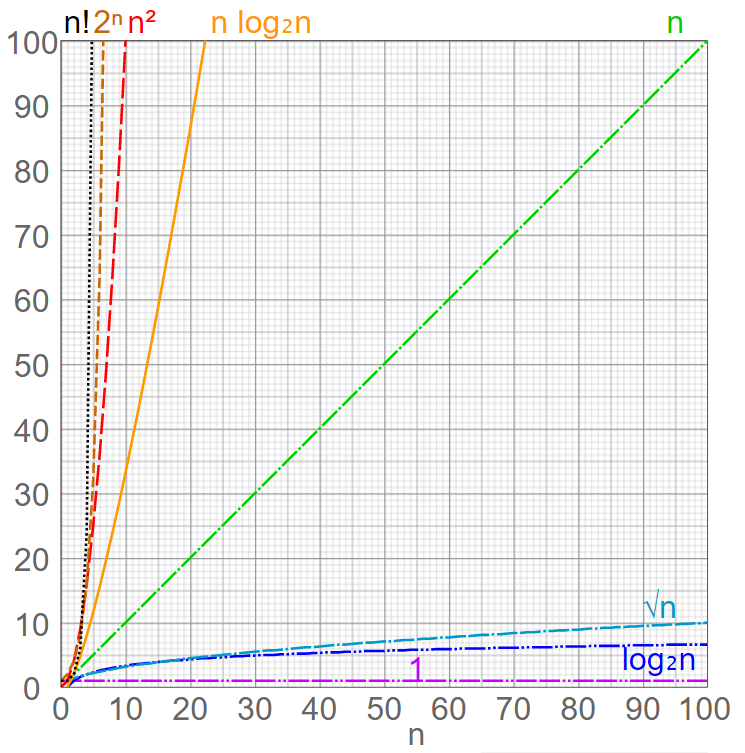
\includegraphics[width= 0.6\textwidth]{comp.png} \]             


\subsection{Algorithm Efficiency vs. Computer Power}
Computers are improving all the time, and tasks that would take hours on the earliest computers can be done in seconds today. However, these improvements primarily apply to algorithms that are relatively efficient. As the run time complexity (represented by its big $O$ class) of an algorithm gets worse, the effect of an increase in raw computation power becomes less significant. 

The first thing to understand is that the problems with inefficient algorithms come up when the input size is relatively large. For very small inputs, for example, the worst case time complexity of an `inefficient' algorithm might be better than that of an `efficient one'. We generally don't consider this to be important from a theoretical standpoint, because for small enough inputs our computers just blast through the problems basically whatever algorithm we use (so long as it's not ridiculous). What happens with inefficient algorithms is that as the input size increases they quickly `hit a wall', and a small increase in the size of the input suddenly results in a very large increase in the running time of the algorithm. 

This increase means you can go from `computations that can be done in a few seconds' to `computations that take hours or days' just by increasing the input size a little bit. So when we think about computing power for inefficient algorithms, what we want to know is, ``how much bigger can we make the input before the computation time becomes unreasonable?". Of course, people building real computers also care about linear increases in efficiency too, because running an algorithm in half the time can be a big difference in practice, but from the `broad strokes' theory standpoint we don't consider it.      

Anyway, suppose we have an algorithm for solving a given decision problem, suppose we have computers $C_1$ and $C_2$ running this algorithm, and suppose finally that $C_2$ is capable of performing $2^{12}$ computation steps in the time it takes $C_1$ to do 1 (so $C_2$ is 4096 times faster than $C_1$ - in symbols $v_2 = 2^{12}v_1$, where $v_i$ is the number of computation steps machine $C_i$ can take each second). How much improvement does this give us in terms of the size of inputs that can be computed in the same time? The answer depends on the running time of the algorithm. 

Suppose first that the algorithm runs in linear time (i.e. $f$ is $O(n)$, where $f$ is the `worst case run time' function we talked about before). Let $t$ be some fixed amount of time (in seconds). The maximum number of steps it takes $C_1$ to run the algorithm on an input of length $n_1$ is given by $f(n_1)$, and $f(n_1)\leq cn_1$ for some constant $c$, as $f$ is $O(n)$. To guarantee that $C_1$ completes the computation in at most time $t$, we require that $cn_1\leq v_1t$, because $v_1t$ is the maximum number of computation steps $C_1$ can take in time $t$. Rearranging the formula, we must have $n_1\leq \frac{v_1t}{c}$. In other words, the largest input length for which we can guarantee $C_1$ will complete the algorithm within $t$ seconds is $\lfloor \frac{v_1t}{c}\rfloor$. What about $C_2$? 

To answer this, let $v_2$ be the number of computation steps $C_2$ takes every second. Remember that $v_2 = 2^{12}v_1$. Similar to the case of $C_1$, if we want to be sure $C_2$ completes the computation in at most $t$ seconds on an input of length $n_2$, we require $cn_2\leq v_2 t$, which rearranges to give $n_2\leq \frac{v_2t}{c}$. In other words, the largest input length for which we can guarantee $C_2$ will complete the algorithm within $t$ seconds is $\lfloor \frac{2^{12}v_1t}{c}\rfloor$. This is $2^{12}$ times bigger than for $C_1$, so is a huge improvement.

What happens when the algorithm has worse performance? Suppose now the algorithm runs in quadratic time (i.e. $f(n)$ is $O(n^2)$, so $f(n)\leq cn^2$ for some constant $c$). Let $v_1$ and $v_2$ be as before. This time, to guarantee completion in at most time $t$ by $C_1$ on an input of length $n_1$, we must have $cn_1^2\leq v_1t$. In other words, $n_1\leq \sqrt{\frac{v_1t}{c}}$. Similarly, for $C_2$, we must have input length \[n_2\leq \sqrt{\frac{v_2t}{c}}=\sqrt{\frac{2^{12}v_1t}{c}}= 2^6\sqrt{\frac{v_1t}{c}}.\]   
In other words, roughly speaking, the biggest input guaranteed to halt within $t$ seconds on $C_2$ is $2^6$ times bigger than the biggest such input for $C_1$. Another big improvement, but significantly worse than in the linear case.

Suppose now we have a really inefficient algorithm that runs in exponential time (i.e. $f$ is $O(2^n)$). Then we have $2^{n_1}\leq \frac{v_1t}{c}$ and $2^{n_2}\leq \frac{v_2 t}{c}$ for some constant $c$, and by taking logs base 2 this gives $n_1\leq \log(v_1) + \log(t) - \log (c)$, and $n_2\leq \log(v_2) + \log(t) - \log (c)$.
Since $v_2=2^{12}v_1$, the second inequality can be rewritten as 
\begin{align*}n_2&\leq \log(2^{12}v_1) + \log(t) - \log (c)\\
&= \log(2^{12}) +\log(v_1) + \log(t) - \log (c)\\
&= 12 + \log(v_1) + \log(t) - \log (c).\end{align*}
This tells us that the biggest input guaranteed to halt within $t$ seconds on $C_2$ is only 12 bigger than the biggest such input for $C_1$. Not 12 times, just plus 12. This is a very small improvement considering how much faster $C_2$ is than $C_1$. The lesson from this is that faster hardware cannot do much to compensate for truly inefficient algorithms.    


\subsection{Tractability and Intractability}
Complexity theory divides algorithms into rough complexity classes based on their use of resources. We're interested in run time, so the classes we discuss here are based on worst case run time as discussed previously. We've seen how we can define the worst case run time of an algorithm as a function of the size of its input, and we've also introduced big $O$ notation to group algorithms into classes based on the upper bounded run time of their fastest know algorithm (e.g. $O(n)$, $O(n^3)$, $O(2^n)$ etc.). The difference between $O(n^2)$ and $O(n^3)$ is actually very important in applications. For example, in some applications an $O(n^3)$ algorithm might be much too slow, but an $O(n^2)$ algorithm might be manageable. For some applications, e.g. in Big Data, $O(n^2)$ might be much too slow. Despite this, theorists often make a sharp distinction between  `efficient' and `inefficient' algorithms, and between `easy' and `hard' decision problems, based on the following definitions.

\begin{definition}[polynomial time]
An algorithm is polynomial time ($p$-time) if it is $O(n^k)$ for some $k\in\mathbb{N}$.
\end{definition}

\begin{definition}[tractable]
A decision problem is tractable if there is a polynomial time algorithm that decides it. It is \emph{intractable} otherwise. 
\end{definition}

As a rough approximation, complexity theorists consider tractable problems to be `easy', and intractable ones to be `hard'. In practice, a polynomial time algorithm might be much too slow for practical use, as mentioned above. Of course, finding a polynomial time algorithm for a problem, thus demonstrating its `easiness', may not be easy at all!


\subsection{Run Time Vs. Encoding System}
The question of whether a given $n\in\mathbb{N}$ is prime is a simple and important decision problem. Consider the following algorithm:

\begin{verbatim}
Prime(n).

answer = `true'
for i = 2 to n-1
	if i divides n then answer = `false'
return answer.	
\end{verbatim} 

Testing if $i$ divides $n$ is quite fast. Say we have an $O(n^2)$ algorithm for this (just calculate $ij$ for every $1< j\neq i < n$ - I'm not claiming this is the best possible run time for this algorithm). The the worst case running time of the `Prime' algorithm would be $O(n^3)$, as we check if $i$ divides $n$ for every $i$ between $2$ and $n$. However, if we want to run this algorithm on a Turing machine we need to encode natural numbers using a finite alphabet, and the length of the input is the number of symbols we use, not the size of the number. For example, a binary number of length $n$ can represent a natural number up to $2^n-1$. So considered as a function of binary input length this algorithm has a worst case run time of $O((2^n)^3)=O(2^{3n})$, because the length $n$ input might correspond to the number $2^n-1$.  

On the other hand, if we use unary notation then the algorithm does indeed run in $p$-time, as then the length of the input is equal to the size of the number. What this tells us is that there is a relationship between how we encode problems and the running times of algorithms we can use to solve them. We can make algorithms look more efficient by representing the problem in an inefficient way. This is somewhat similar to the relationship between the complexity of encoding systems for Turing machines and the minimum size of universal Turing machines that can simulate them. There we can trade higher complexity of encoding for smaller size of minimal UTM and vice versa. By the way, you shouldn’t take the details of the calculations above too seriously as we were loose with our treatment of the algorithm for checking divisibility, but hopefully the main point is clear.  

It turns out that there are $p$-time algorithms for (binary) primality testing, for example the $AKS$ test, but these use some number theory tricks, and their run times are too slow to be practical in most applications (roughly, a little slower than $O(\log(n)^6)$). In industry people generally use probabilistic algorithms based on mathematical number theory for primality testing. These are much faster, but don't always give the correct answer (though errors can be made very rare).     


\subsection{Polynomial Time Reduction}
Previously we saw how we can order decision problems in terms of their decidability using reduction. That is, $A\leq B$ if there's an algorithm that turns `yes' instances of $A$ into `yes' instances of $B$, and `no' instances of $A$ into `no' instances of $B$. The notation comes from the fact that, if such an algorithm exists, then we could use an algorithm for solving $B$ to solve $A$ too, so problem $B$ is `at least as hard' as problem $A$.

We can extend the idea of reduction to order decision problems in terms of their polynomial time solvability. We write $A\leq_p B$ if there is a $p$-time algorithm that turns `yes' instances of $A$ into `yes' instances of $B$, and `no' instances of $A$ into `no' instances of $B$. Then, if we had a $p$-time algorithm for solving $B$ we could combine it with the $p$-time conversion algorithm to get a $p$-time algorithm for solving $A$.

Actually there is a complication here. Our first algorithm converts instances of $A$ to instances of $B$ in $p$-time, and the second algorithm solves $B$ in $p$-time. But the second algorithm runs in $p$-time on the size of its input, and the algorithm that converts instances of $A$ to instances of $B$ does not necessarily preserve their sizes. So, if the first algorithm dramatically increases the size of an instance of $A$ while converting it then, even though the second algorithm runs in $p$-time on the converted input, we might worry that it could end up running slower than $p$-time on the size of the original instance of $A$. 

Fortunately, this is not a problem because the fact that the conversion algorithm is $p$-time bounds the size of the converted instance. I.e. if the conversion algorithm runs in time $n^k$ for some $k$ and the original $A$ instance has size $m$, then the converted instance can be at most size $cm^k$ for some constant $c$. Then, if the algorithm for solving $B$ is $O(n^l)$ for some $l$, the worst case run time for converting this instance of $A$ to an instance of $B$ then solving with the algorithm for $B$ is $O((n^k)^l)=O(n^{kl})$, which is $p$-time.    

\begin{exercise}
Why is it obvious that $\leq_p$ is reflexive?
\end{exercise}

\begin{theorem}
$\leq_p$ is transitive.
\end{theorem}
\begin{proof}
Suppose $A\leq_p B$ and $B\leq_p C$. If $I$ is an instance of $A$ let $f(I)$ be the result of applying the reduction of $A$ to $B$ to $I$. Similarly, if $J$ is an instance of $B$ let $g(J)$ be the result of applying the reduction of $B$ to $C$ to $J$. We can compose $f$ and $g$ as functions, so $g(f(I))$ is a reduction of $A$ to $C$. We need to check $g\circ f$ is $p$-time. Suppose the reduction of $A$ to $B$ is $O(n^k)$ for some $k$, and the reduction from $B$ to $C$ is $O(n^l)$ for some $l$. Then the maximum size of $f(I)$ is $O(n^k)$, so $g\circ f$ is $O((n^k)^l)=O(n^{kl})$. So $g\circ f$ is $p$-time as required.
\end{proof}

\begin{theorem}\label{T:Pmin}
Let $A$ and $B$ be decision problems. Then, if there is a $p$-time algorithm for solving $A$, and if $B$ has at least one `yes' instance and at least one `no' instance, then $A\leq_p B$.
\end{theorem}
\begin{proof}
Since there's a $p$-time algorithm for solving $A$, to convert instances of $A$ to instances of $B$ we just use the $p$-time algorithm to check if they are `yes' or `no' instances of $A$ then convert them to either the `yes' or `no' instance of $B$ appropriately. This `conversion' is constant time,  as we always convert to either the fixed `yes' instance, or the fixed `no' instance. 
\end{proof}

We know that $\leq_p$ is not symmetric, because if $\leq_p$ were symmetric it would follow from theorem \ref{T:Pmin} that every decision problem would have a $p$-time solution. Since there are problems that are not even decidable this is impossible. However, we can use $\leq_p$ to define a relation between decision problems that is reflexive, transitive, and symmetric (i.e. an equivalence relation).

\begin{definition}[$\equiv_p$]
Decision problems $A$ and $B$ are \emph{$p$-time equivalent} if $A\leq_p B$ and $B\leq_p A$.
\end{definition} 


\subsection{Example - The Hamiltonian Circuit Problem and the Traveling Salesman Decision Problem}
We consider two decision problems and show that one is $p$-time reducible to the other.

\begin{definition}[Hamiltonian circuit] 
Given a finite simple graph $G$ with $n$ vertices, a Hamiltonian circuit is a sequence $c=(v_1,v_2,\ldots,v_n)$ such that
\begin{enumerate}
\item if $v_i$ and $v_j$ occur consecutively in the sequence then there is an edge from $v_i$ to  $v_j$ in $G$,
\item every vertex of $G$ occurs in $c$, and
\item there is an edge from $v_n$ to $v_1$.  
\end{enumerate}  
\end{definition}

Informally a Hamiltonian circuit is a path in $G$ that passes through every vertex exactly once before returning to its origin.

\begin{definition}[$HCP$]
The Hamiltonian circuit problem ($HCP$) is whether a given finite undirected simple graph has a Hamiltonian circuit.
\end{definition}

\begin{definition}[weighted graph]
A weighted graph is a graph where every edge is associated with a number (usually a non-negative integer). This number can be thought of as the `cost' of traveling along that edge.
\end{definition}

\begin{definition}[$TSDP$]\label{D:TSDP}
The traveling salesman decision problem ($TSDP$) has instances $(G,d)$, where $G$ is a finite complete undirected weighted simple graph with non-negative integer weights, and $d$ is a non-negative integer. The question is whether there is a Hamiltonian circuit in $G$ such that the sum of the weights of the edges used in the circuit is less than or equal to $d$. 
\end{definition}

\begin{theorem}\label{T:TSDPtoHCP}
$HCP\leq_p TSDP$, where the reduction is $p$-time when considered as a function of the number of vertices plus the number of edges of the instance graph $G$.
\end{theorem}
\begin{proof}
An instance of $HCP$ is a finite undirected simple graph $G$ with $n$ vertices and $e$ edges. We will convert $G$ into a pair $(G',d)$ where $G'$ is a finite complete undirected weighted simple graph, and $d$ is a non-negative integer. This is an instance of $TSDP$. We then show that `yes' instance of $HCP$ become `yes' instances of $TSDP$, and similar for `no' instances. Finally we check that the conversion algorithm runs in $p$-time as a function of $n+e$.

Let $G'$ have the same vertices as $G$. To be an instance of $TSDP$ $G'$ must be complete, so we add edges for pairs of vertices. We now weight the edges so that the edges between vertices that are connected by an edge in $G$ have weight 0, and the rest have weight $1$. We set $d=0$. So $G'$ has a Hamiltonian circuit with total weight 0 if and only if there is a Hamiltonian circuit in $G$ (because the edges with weight 0 in $G'$ are precisely the edges of $G$). This shows the reduction is correct.

How fast is the reduction? Well, we have to clone the vertices of $G$. Assuming it takes constant time to clone a single vertex, doing this for every vertex will take linear time. I.e. $O(|V|)$, where $V$ is the set of vertices of $G$. Then we add edges for pairs of vertices. There are $n \choose 2$ pairs of vertices of $G$, so assuming it takes constant time to add a single edge, doing this for every pair takes quadratic time. I.e. $O(|V|^2)$. Setting the weights involves checking every edge of $G'$ to see if it corresponds to an edge of $G$. We can do this naively just by checking every edge of $G$ to see if it is an edge between $v$ and $v'$ for every pair $v,v'\in V$. This is $O(|E|\times|V|^2)$, where $E$ is the set of edges of $V$. Finally, setting $d=0$ is a constant time operation, say $c$. So the whole process takes $O(|V|)+O(|V|^2)+O(|E|\times|V|^2)+c$, which is $O((|V|+|E|)^3)$ at most. This is $p$-time as required.  
\end{proof}

The converse to the theorem above is also true. If you are feeling ambitious you can try to prove it directly using $p$-time reduction. This direction is harder than the direction proved in the theorem. We will prove it using some powerful general theory at the end of the course.



\end{document}
\subsection{Exercises}
\documentclass{article}

\usepackage{amsmath, mathrsfs, amssymb, stmaryrd, cancel, relsize,tikz,amsthm,comment,enumerate}

\theoremstyle{definition}
\newtheorem{Q}{Question}
\newtheorem{definition}{Definition}

\newcommand{\tvs}{\textvisiblespace}
\newcommand{\ra}{\rightarrow}
\newcommand{\la}{\leftarrow}
\newcommand{\co}{\mathbf{code}}

%\includecomment{comment}


\title{ITCS 532 Foundations of Computer Science\\
Week 6 - Tractability and $p$-Time Reduction (Homework)}
\author{Rob Egrot}
\date{}

\begin{document}
\maketitle

\begin{Q}
Prove that $\equiv_p$ is an equivalence relation.
\end{Q}
\begin{comment}
\textbf{Solution}
We know $\leq_p$ is reflexive by exercise 7.5.1 in the notes, so clearly $A\equiv_p A$. We also know $\leq_p$ is transitive by theorem 7.5.2, so if $A\equiv_p B$ and $B\equiv_p C$, then by definition of $\equiv_p$ we have $A\leq_p B$ and $B\leq_p C$, so $A\leq_p C$. Similarly we have $C\leq_p A$ and so $A\equiv_p C$. So $\equiv_p$ is transitive. Finally, $A\equiv_p B \iff A\leq_p B$ and $B\leq_p A$, and so $\equiv_p$ is obviously symmetric.
\end{comment}

\begin{Q}
Let $k\in \mathbb{N}\setminus\{0\}$.
\begin{enumerate}[a)]
\item Prove that $k^{n+1}$ is $O(k^n)$ as a function of $n$.
\item Prove that $k^{2n}$ is not $O(k^n)$ as a function of $n$.
\end{enumerate}
\end{Q}
\begin{comment}
\textbf{Solution}
\begin{enumerate}[a)]
\item We have $k^{n+1} = k.k^n $ for all $n$. So $k^{n+1}\leq ck^n$ when $c=k$. I.e. $k^{n+1}$ is $O(k^n)$.
\item Suppose $k^{2n}$ is $O(k^n)$. Then there is a constant $c$ with $k^{2n}\leq ck^n$ for `large' $n$. Taking $\log_k$ of both sides gives
\[2n\leq \log_k c + n,\]
and so
\[n \leq \log_k c,\]
but this obviously cannot be true for all `large' $n$. 

\end{enumerate}
\end{comment}

\begin{Q}
Let $C_1$ and $C_2$ be computers, and suppose that $C_2$ is $2^9$ times faster than $C_1$. I.e. if $C_1$ can take $v_1$ computation steps per second then $C_2$ can take $v_2=2^9v_1$ computation steps per second. $C_1$ and $C_2$ both run the same $O(n^3)$ algorithm for sorting a list of numbers of size $n$. Suppose the largest list size that $C_1$ can guarantee to sort in some fixed time $t$ is 1000. I.e. $C_1$ can guarantee to sort a list with size at most 1000 in time $t$ (a whole number of seconds), but larger lists may take longer. Approximately what is the largest list size that $C_2$ is guaranteed to sort in the same time $t$?  
\end{Q}
\begin{comment}
\textbf{Solution}
Let $n_i$ be the largest list size that $C_i$ is guaranteed to sort within time $t$, for $i\in\{1,2\}$. Since the algorithm is $O(n^3)$, there is a constant $c$ such that the run time on a list of length $n$ is at most $cn^3$. The number of computation steps $C_i$ can take in time $t$ is $v_it$. So $n_i = \max \{n : cn^3\leq v_it\}$. I.e. $n_1 = \lfloor (\frac{v_1t}{c})^{\frac{1}{3}} \rfloor$, and $n_2 = \lfloor (\frac{v_2t}{c})^{\frac{1}{3}} \rfloor$. But $v_2 = 2^9v_1$, and so $n_2 = \lfloor (\frac{2^9v_1t}{c})^{\frac{1}{3}} \rfloor \approx 2^3\lfloor (\frac{v_1t}{c})^{\frac{1}{3}} \rfloor = 2^3n_1$. We are told $n_1 = 1000$, so $n_2\approx 2^3\times 1000 = 8000$. 

  
\end{comment}

\begin{Q}
\emph{This question is to review the technique of reduction (not $p$-time reduction, just ordinary reduction).} Let $\Sigma = \{0,1\}$. Let $D$ be the decision problem ``Given a Turing machine $T$ over $\Sigma$, does $T(I)$ halt whenever $|I|$ is odd?". 
\begin{enumerate}[a)]
\item Define the empty tape halting problem ($ETHP$).
\item Show that $ETHP \leq D$.
\item Is $D$ decidable? Justify your answer.
\end{enumerate}
\end{Q}
\begin{comment}
\textbf{Solution}
\begin{enumerate}[a)]
\item ``Given a Turing machine $T$, does $T$ halt when run on a blank tape?''.
\item An instance of $ETHP$ is a Turing machine $T$. An instance of $D$ is also a Turing machine. Given a Turing machine $T$ we will construct $T'$ such that $T$ halts on the empty input iff $T'(I)$ halts whenever $|I|$ is odd. $T'$ operates on an input $I$ as follows:
\begin{enumerate}[1)]
\item First $T'$ erases $I$ and moves the tape head back to the start of the tape.
\item $T'$ then does what $T$ do (note the tape is now empty).
\end{enumerate}
Then $T(\epsilon)$ halts implies $T'(I)$ halts for all $I$, so also whenever $|I|$ is odd. Conversely, $T'$ does the same thing for all inputs, and $T'(I)$ halts for all $I$ with $|I|$ odd implies $T(\epsilon)$ halts.
\item We conclude that $D$ is undecidable. As $ETHP\leq D$, an algorithm solving $D$ would imply an algorithm solving $ETHP$, which is impossible, as $ETHP$ is undecidable.
\end{enumerate}
\end{comment}

\end{document}
\newpage

\section{More $p$-Time Reduction, and an Introduction to $\NP$}
\documentclass{article}

\usepackage{amsmath, mathrsfs, amssymb, stmaryrd, cancel, relsize,tikz,amsthm}
\usepackage[all]{xy}
\theoremstyle{plain}
\newtheorem{theorem}{Theorem}[section]{\bfseries}{\itshape}
\newtheorem{proposition}[theorem]{Proposition}{\bfseries}{\itshape}
\newtheorem{definition}[theorem]{Definition}{\bfseries}{\upshape}
\newtheorem{lemma}[theorem]{Lemma}{\bfseries}{\upshape}
\newtheorem{corollary}[theorem]{Corollary}{\bfseries}{\upshape}
\newtheorem{exercise}[theorem]{Exercise}{\bfseries}{\upshape}

\theoremstyle{definition}
\newtheorem{example}[theorem]{Example}{\bfseries}{\upshape}

\newcommand{\tvs}{\textvisiblespace}
\newcommand{\ra}{\rightarrow}
\newcommand{\la}{\leftarrow}
\newcommand{\co}{\mathbf{code}}
\newcommand{\Po}{\mathbf{P}}
\newcommand{\NP}{\mathbf{NP}}
\newcommand{\bbN}{\mathbb{N}}
\newcommand{\SAT}{\mathsf{PSAT}}



\title{ITCS 532 Foundations of Computer Science\\
Class 7 - More on $p$-time reduction, and an introduction to $\NP$}
\author{Rob Egrot}
\date{}

\begin{document}
\maketitle
\subsection{Example - The Directed Hamiltonian Circuit Problem}
\begin{definition}[DHCP]
The directed Hamiltonian circuit problem ($DHCP$) asks whether a given finite \emph{directed} simple graph has a Hamiltonian circuit. A Hamiltonian circuit in a directed graph is like a Hamiltonian circuit in an undirected graph except we take the edge directions into account. 
\end{definition}

\begin{theorem}
$HCP\leq_p DHCP$, where the reduction is $p$-time when considered as a function of the number of edges plus the number of vertices of the instance graph $G$.
\end{theorem}
\begin{proof}
This is an easy proof. We start with a finite undirected simple graph $G=(V,E)$ and we want to construct a finite directed simple graph $G'$ in $p$-time such that $G$ has a Hamiltonian circuit if and only if $G'$ does. In our construction the vertices of $G'$ are copies of the vertices of $G$, and for every undirected edge in $G$ we add two directed edges to $G'$ between the same vertices (one in each direction). $G'$ has the same vertices as $G$, and for every edge of $G$ we add two to $G'$. Assuming adding vertices and edges takes constant time this means that the construction of $G'$ is actually linear time ($O(m)$ if $m=|V|+|E|$). 

We must check the construction of $G'$ preserves `yes' and `no' instances correctly. $G$ is a yes instance if and only if it has a Hamiltonian circuit $v_1,v_2,\ldots,v_n$. By construction of $G'$, if $v_1,v_2,\ldots,v_n$ is a Hamiltonian circuit in $G$ then there are directed edges in $G'$ from $v_i$ to $v_{i+1}$ for all $i=1,2,\ldots,n-1$, and also from $v_n$ to $v_1$. So $v_1,v_2,\ldots,v_n$ is also a Hamiltonian circuit in $G'$. Conversely, if $v_1,v_2,\ldots,v_n$ is a Hamiltonian circuit in $G'$ then there must be edges in $G$ connecting $v_i$ and $v_{i+1}$ for all $i=1,2,\ldots,n-1$, and also an edge connecting $v_n$ and $v_1$. So $v_1,v_2,\ldots,v_n$ is also a Hamiltonian circuit in $G$ as required.     
\end{proof}

\begin{theorem}
$DHCP\leq_p HCP$, where the reduction is $p$-time when considered as a function of the number of vertices plus the number of edges of the instance graph $G$.
\end{theorem}
\begin{proof}
This direction is not easy. We start with a directed simple graph $G$ and we must construct an undirected  simple graph $G'$ in $p$-time that preserves `yes' and `no' instances. This is hard because it's not at all obvious how to encode the direction of edges of $G$ in $G'$. This is a problem because a Hamiltonian circuit in $G$ must travel along edges in the right direction. If we lose information about the direction of edges then Hamiltonian circuits in $G'$ may not correspond to Hamiltonian circuits in $G$. Fortunately, with some thought we can overcome this problem.

If $V$ and $E$ are the sets of vertices and edges of $G$ respectively, we define $G'=(V',E')$ as follows:
\begin{itemize}
\item $V'=\bigcup\{\{v,v^I,v^O\}:v\in V\}$
\item $E'=\{\{v_0^O,v_1^I\} : (v_0,v_1)\in E\} \cup \{\{v,v^I\},\{v,v^O\}:v\in V\}$
\end{itemize}

The idea is that every vertex $v$ of $G$ gets two partner vertices, $v^I$ and $v^O$, that will be used to encode the direction of edges. There are edges in $G'$ connecting $v$ to $v^O$ and $v^I$, and wherever there's a directed edge $(v,v')$ between vertices in $G$ there's an edge between $v^O$ and $v'^I$ in $G'$. E.g.
\[\xymatrix{
\ar[dr]& & &\\
& \bullet_{v_0}\ar[r] &\bullet_{v_1}\ar[ur]\ar[dr] & \\
\ar[ur] & & &}\]
becomes 
\[\xymatrix{
\ar@{-}[dr] & & & & & & & &\\
& \bullet_{v_0^I}\ar@{-}[r] & \bullet_{v_0}\ar@{-}[r] & \bullet_{v_0^O}\ar@{-}[r] & \bullet_{v_1^I}\ar@{-}[r] & \bullet_{v_1}\ar@{-}[r] & \bullet_{v_1^O}\ar@{-}[ur]\ar@{-}[dr]\\
\ar@{-}[ur] & & & & & & & &}\]

We need to show that $G$ has a Hamiltonian circuit if and only if $G'$ does. If $|V|=n$ and $v_1,v_2,\ldots,v_n$ is a Hamiltonian circuit in $G$, then 
\begin{equation*}v^I_1,v_1, v^O_1, v_2^I, v_2, v_2^O,\ldots,v_n^I,v_n,v_n^O\end{equation*} is a Hamiltonian circuit in $G'$. 

Conversely, if $|V|=n$ then $|V'|=3n$. Suppose $c=u_1,u_2,\ldots,u_{3n}$ is a Hamiltonian circuit in $G'$. Then every $v\in V$ appears somewhere in $c$. But for each $v\in V$, the only edges connecting $v$ are $\{v,v^I\}$ and $\{v,v^O\}$. Since $|V|=n$ and $c$ has exactly $3n$ elements, a simple counting argument tells us that, after choosing a suitable starting point, $c$ must have form \[v^{x_0}_1,v_1, v^{y_0}_1, v_2^{x_1}, v_2, v_2^{y_1},\ldots,v_n^{x_n},v_n,v_n^{y_n}\] for some labeling of the vertices in $V$. Here for all $i\in\{1,\ldots,n\}$ we have $x_i,y_i\in\{I,O\}$.

Now, since there are no edges in $G'$ of the form $(v_i^I,v_j^I)$, or $(v_i^O,v_j^O)$ we must have either  \begin{equation*}c= v^I_1,v_1, v^O_1, v_2^I, v_2, v_2^O,\ldots,v_n^I,v_n,v_n^O,\end{equation*} or \begin{equation*}c=v^O_1,v_1, v^I_1, v_2^O, v_2, v_2^I,\ldots,v_n^O,v_n,v_n^I.\end{equation*} So by the construction of $G'$, we get a Hamiltonian circuit in $G$ by either following $c$ forwards or backwards.

We still have to check the reduction is $p$-time in the number of edges of $G$. First we constructed the vertices of $G'$. There are three of these for every vertex of $G$, so this step runs in $O(|V|)$ time. Then we added edges of form $(v^I,v)$ and $(v,v^O)$ for every vertex of $G$. Again this is $O(|V|)$. Finally we added edges of form $(u^O,v^I)$ for every edge of $G$. This is obviously $O(|E|)$, to so the combined running time is also $O(|V|+|E|)$, which is $p$-time as claimed.
\end{proof}

\subsection{Verifiers}
It is a well known basic fact of number theory that every natural number can be written as a product of prime numbers in an essentially unique way (that is, it's unique except for the order we write the primes). This fact is known as the \emph{Fundamental Theorem of Arithmetic}. So, given a natural number $n$, an obvious question is, `what is the prime decomposition of $n$?'. This is not, in general, an easy question to answer. In fact, no $p$-time algorithm is known. On the other hand, it \emph{is} easy to check whether the product of a given collection of prime numbers is equal to a particular number (just multiply them all together and look at the result). This illustrates an important principle: For some questions it's hard to find a solution, but it's easy to check whether a proposed solution is correct. In the case of the prime factorization problem, this asymmetry lies at the heart of RSA encryption.

We can formalize this in terms of decision problems and Turing machines with something called a \emph{verifier}.

\begin{definition}[Verifier]
Given a language $L$ over a finite alphabet $\Sigma$, a verifier for $L$ is a modified Turing machine $V$, where $V$ takes two inputs instead of one (consider the inputs to be separated by a special symbol), and such that
\[x\in L\iff \text{ there is } y\in\Sigma^* \text{ such that } V(x,y) \text{ accepts}\]
Here $y$ is called a \emph{certificate} for $x$. A verifier must halt for all inputs. We say a verifier for $L$ runs in $p$-time if it runs in $p$-time with respect to the length of $x$ for all inputs $(x,y)$.  
\end{definition}
The certificate is like a proposed solution. The verifier accepts $x$, which encodes an instance of a decision problem, if and only if there's some proposed solution $y$ that it can check is actually a solution. 

\begin{example}[Composite numbers]
We could build a verifier to check if numbers are composite (i.e. not prime). Here the certificates would be potential non-trivial divisors. $V$ would run by checking whether $y$ non-trivially divides $x$ (so we exclude $y=1$ or $y=x$). If so $V(\co(x),\co(y))$ would accept, and if not it would reject.
\end{example}  

\begin{example}[Hamiltonian circuits]
An instance of the Hamiltonian circuit problem is a graph $G$. A certificate for $G$ is just a sequence $s$ of vertices (in coded form). A verifier $V$ for the Hamiltonian  circuit problem would accept on input $(\co(G),\co(s))$ if and only if $s$ defines a Hamiltonian circuit in $G$. 
\end{example}

If we don't care about run time, then verifiers don't really add anything to our toolkit for describing languages, as the theorem below demonstrates. However, when we do care about run times this changes, as we see in the following sections.
\begin{theorem}
A language has a verifier if and only if it is recursively enumerable.
\end{theorem}
\begin{proof}
First let $L$ be an r.e. language and let $T$ be a TM that semidecides $L$. We construct a verifier $V_T$ so that when $V_T$ runs on $(x,\co(n))$, where $n$ is a natural number, it follows the computation $T(x)$ for $n$ steps. It accepts if $T(x)$ accepts within $n$ steps, and rejects otherwise. $V_T$ is clearly a verifier for $L$ because 
\begin{align*}
V_T(x,\co(n))\text{ halts for some }n & \iff T(x)\text{ halts within $n$ steps for some $n$}\\
&\iff T(x) \text{ halts}\\
& \iff x\in L,
\end{align*}
and, moreover, $V_T(x,y)$ halts for all $(x,y)$, assuming it rejects if $y$ is not the code of a natural number. 

For the converse, let $L$ have a verifier $V$. We construct a Turing machine $T_V$ such that $T_V(x)$ operates by generating strings $y$ in lexicographic order and computing $V(x,y)$, and halting if $V(x,y)$ accepts. Then $T_V$ semidecides $L$ because $x\in L$ if and only if there is $y$ such that $V(x,y)$ accepts, and, as $T_V$ computes $V(x,y)$ for every $y$ eventually, it will halt if and only if $x\in L$.   
\end{proof}


\subsection{Complexity Classes}
\begin{definition}
We say that languages/decision problems are in the complexity class $\Po$ if there is a Turing machine that decides them in $p$-time. We say languages/decision problems are in the complexity class $\NP$ if they have a verifier that runs in $p$-time.
\end{definition}

The distinction between $\Po$ and $\NP$ formalizes the distinction between problems that can be efficiently solved, and problems whose solutions can be efficiently checked. As is often the case in complexity theory, these classes are rather coarse. There's a big difference between a problem with a linear time solution, and a problem with an $O(n^{10,000,000})$ solution, but we gloss over it.

Now, we have defined $\Po$ and $\NP$ in terms of kinds of Turing machines, and, as we have seen, there are many variant definitions we could use (e.g. multi-tape etc.). We have seen already that these are equivalent to the `standard' definition in terms of what problems they can decide, but this does not prove that using a different model of computation could not affect which problems are in $\Po$ and $\NP$. For example, we know a problem that can be solved by a `standard' Turing machine could likely be solved in fewer steps by a Turing machine with more tapes. Could this speed increase be such that there is a problem solvable in $p$-time by a multi-tape machine that is not solvable in $p$-time by a `standard' machine? 

The answer turns out to be no, because, if we carefully analyze the modeling of multi-tape Turing machines by single-tape Turing machines from Section \ref{S:TMvar}, we see that, while the single-tape machine takes more steps, the number of steps taken is polynomially bounded by the number of steps the multi-tape machine takes. Therefore, a problem that is $p$-time for a multi-tape machine will also be $p$-time for a single tape machine. The same is true for the other Turing machine variants too. This means our definitions for $\Po$ and $\NP$ are \emph{robust} in the sense that they do not depend unreasonably on the definition of `Turing machine'.     

Note that $\NP$ does \emph{not} stand for \emph{non-polynomial}. This is a common but understandable misconception. $\NP$ actually stands for \emph{non-deterministic polynomial}. The name comes from an alternative definition of the class $\NP$, which we explain in the next section.
\end{document}
\subsection{Exercises}
\documentclass{article}

\usepackage{amsmath, mathrsfs, amssymb, stmaryrd, cancel, relsize,tikz,amsthm,comment,enumerate}

\theoremstyle{definition}
\newtheorem{Q}{Question}
\newtheorem{definition}{Definition}

\newcommand{\tvs}{\textvisiblespace}
\newcommand{\ra}{\rightarrow}
\newcommand{\la}{\leftarrow}
\newcommand{\co}{\mathbf{code}}

%\includecomment{comment}


\title{ITCS 532 Foundations of Computer Science\\
Week 7 - More on $p$-Time Reduction, and an Introduction to $\mathbf{NP}$ (Homework)}
\author{Rob Egrot}
\date{}

\begin{document}
\maketitle
\begin{definition}[Hamiltonian path]
A Hamiltonian path is like a Hamiltonian circuit except that there does not need to be an edge connecting $v_n$ and $v_1$.
\end{definition}

\begin{definition}[$HPP$]
The Hamiltonian path problem ($HPP$) asks whether a given finite undirected simple graph contains a Hamiltonian path.
\end{definition}

\begin{Q}
Let $G=(V,E)$ be a finite undirected simple graph. We construct a new undirected simple graph $G'=(V',E')$ as follows:
\begin{enumerate}
\item $V'=V\cup\{v'\}$ for some $v'\notin V$.
\item $E'= E\cup \{\{v,v'\}:v\in V\}$
\end{enumerate}
I.e. The vertices of $G'$ are those of $G$ with a single new one $v'$. The edges of $G'$ are those of $G$ but with extra edges connecting $v'$ to every vertex of $G$.
\begin{enumerate}[a)]
\item Show that the construction of $G'$ takes polynomial time as a function of $|V|+|E|$.
\item Prove that $G$ has a Hamiltonian path if and only if $G'$ has a Hamiltonian circuit.
\item Deduce that $HPP\leq_p HCP$.
\end{enumerate}
\end{Q}
\begin{comment}
\textbf{Solution}
\begin{enumerate}[a)]
\item If we assume creating a vertex takes constant time, then the time it takes to create the vertices of $G'$ is a constant multiple of $|V|+1$, and so is $O(|V|)$. Similarly, we must create an edge for every edge of $G$, and also new edges for every vertex of $G$. Again, assuming constant time for edge creation, this is $O(|E|+|V|)$. So total time is $O(|V|)+O(|E|+|V|)$, which is $O(|E|+|V|)$.
\item Suppose $v_0,\ldots,v_n$ is a Hamiltonian path in $G$. Then $v_0,\ldots,v_n,v'$ is a Hamiltonian circuit in $G'$. Conversely, suppose $v_0,\ldots,v_n,v_{n+1}$ is a Hamiltonian circuit in $G'$, and suppose without loss of generality that $v_{n+1} = v'$. Then $v_0,\ldots,v_n$ is a Hamiltonian path in $G$.
\item We have found a $p$-time reduction of $HPP$ to $HCP$, and so $HPP\leq_p HCP$ by definition.
\end{enumerate}
\end{comment}

\begin{Q}
Prove that $HCP\leq_p HPP$.
\end{Q}
\begin{comment}
\textbf{Solution}
We construct a new undirected simple graph $G'=(V',E')$ as follows:
\begin{enumerate}
\item Pick a vertex $v$ of $G$. Define new vertices $v',v_0,v_1$.
\item $V'=V\cup\{v',v_0,v_1\}$.
\item $E'=E\cup \{\{v,v'\},\{v_0,v_1\}\}\cup \{\{v_0,u\}:\{v,u\}\in E\}$. 
\end{enumerate}
I.e. We add three new vertices to $G$. We add edges connecting $v$ to $v'$, and $v_0$ to $v_1$, and we also add edges connecting $v_0$ to every vertex $u$ that has edge connecting it to $v$.
Here's a sketch:
\[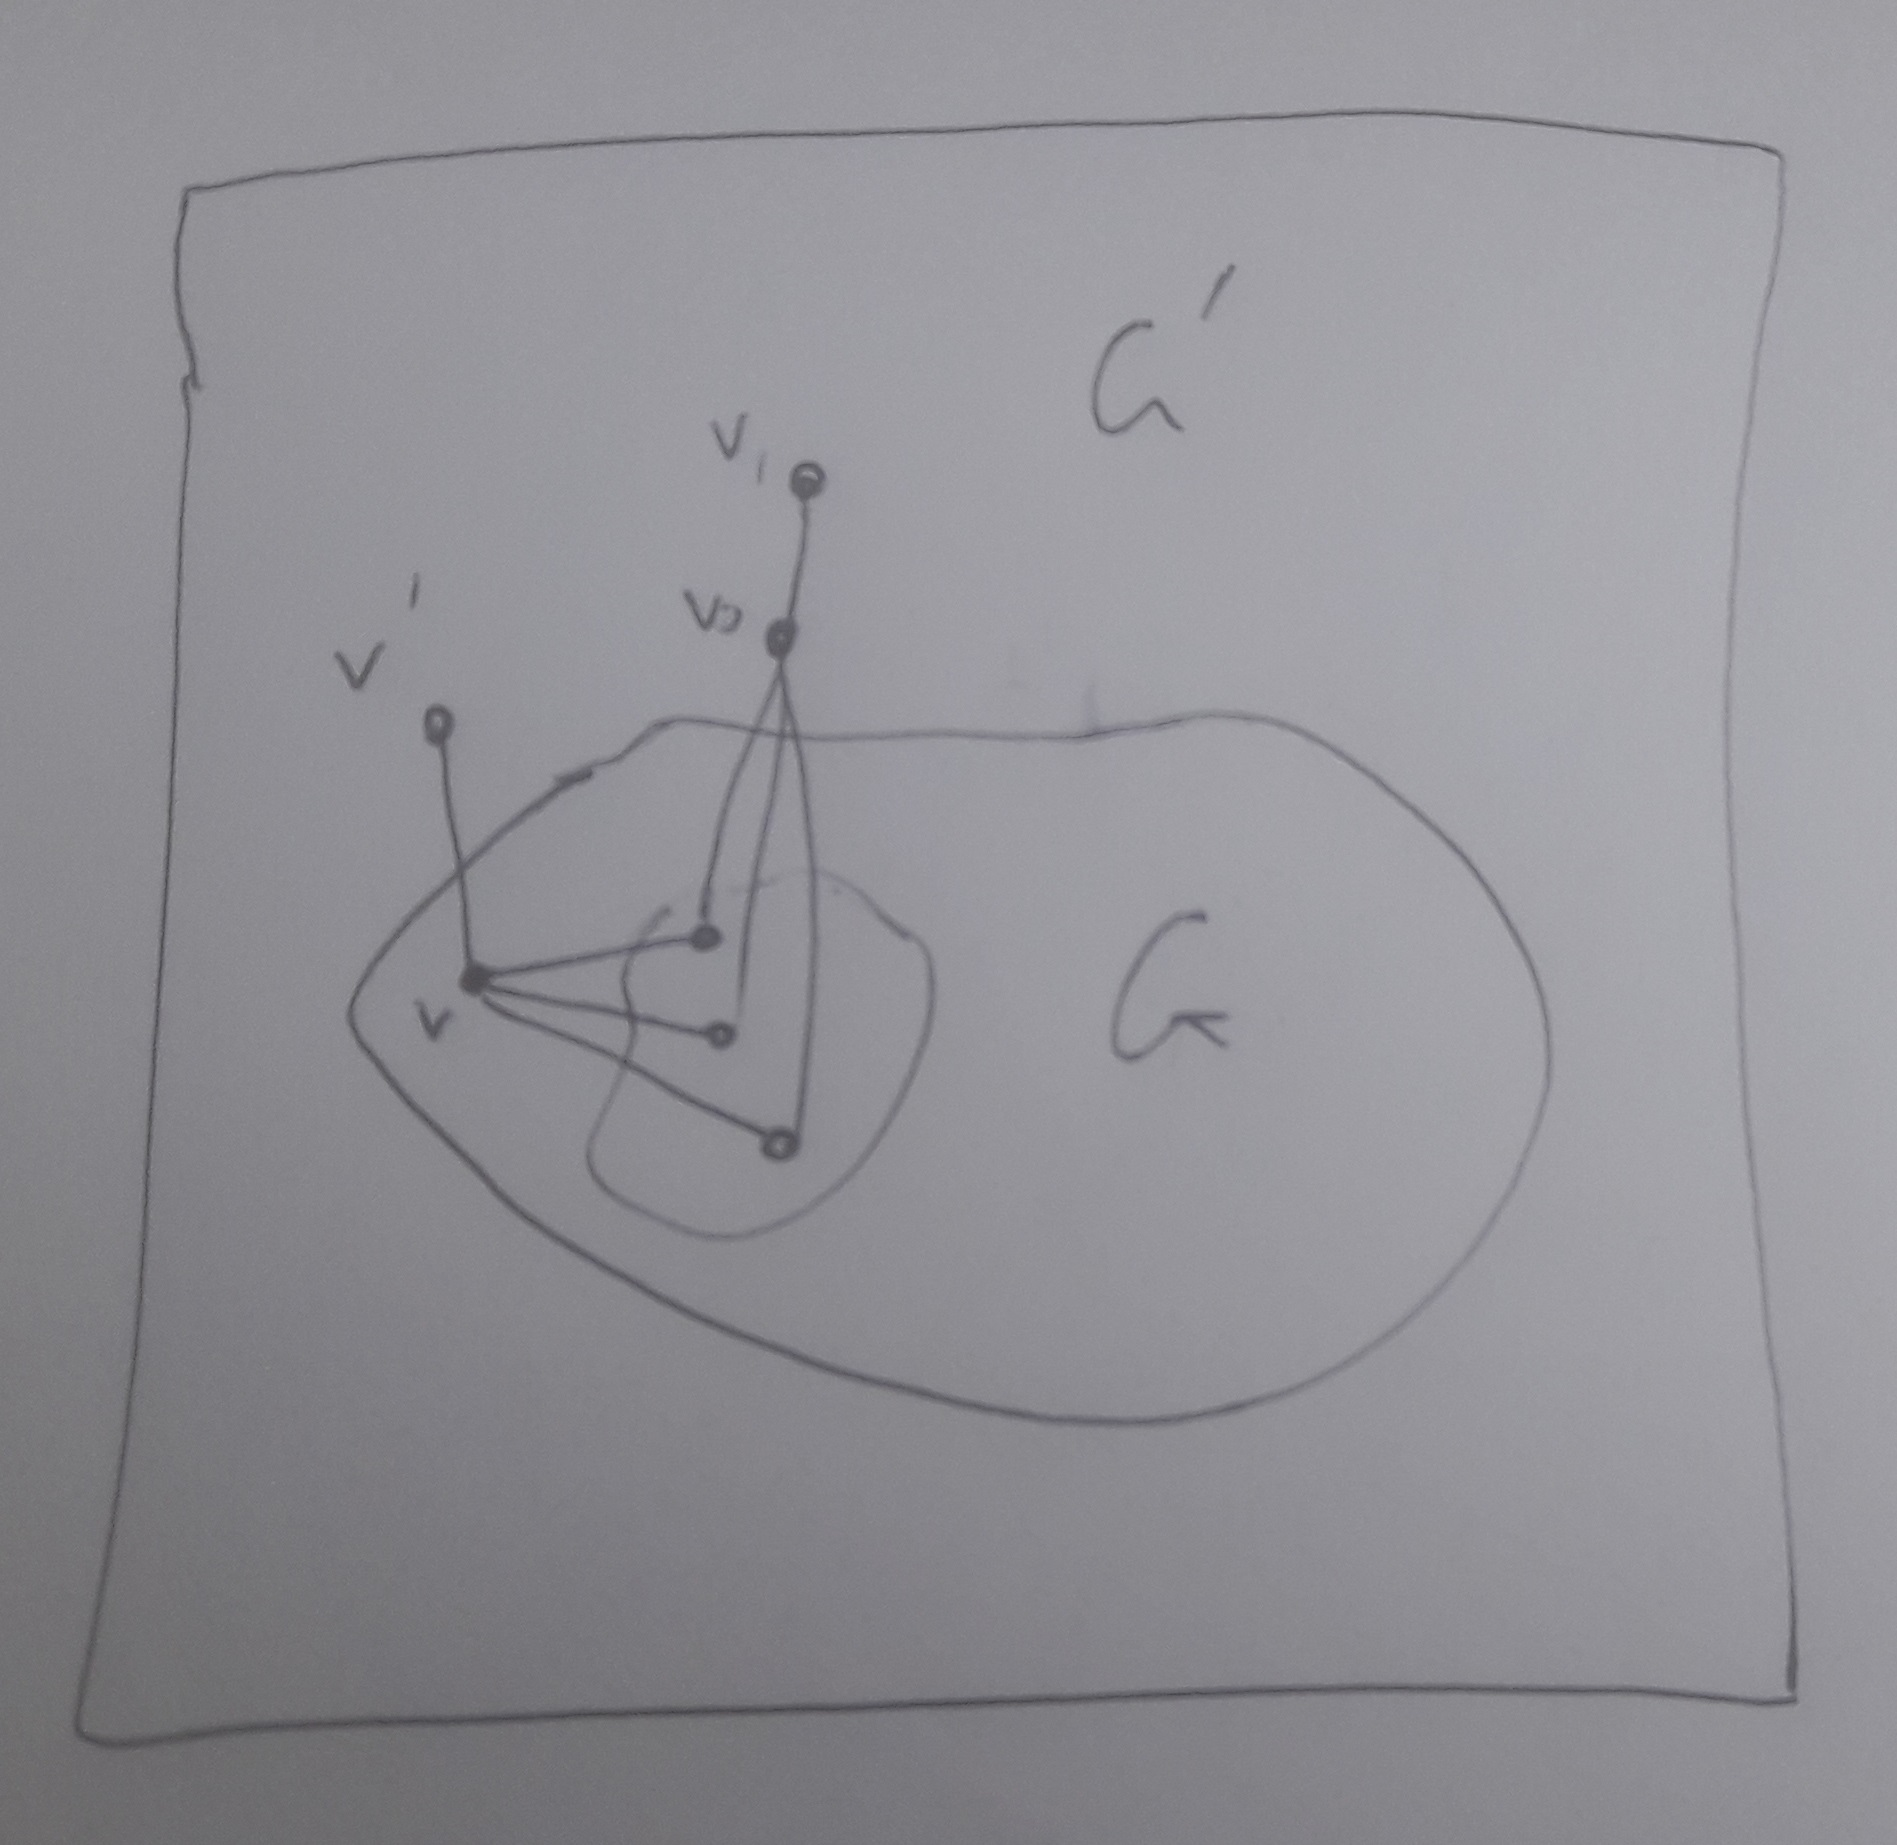
\includegraphics[scale = 0.1]{G.jpg}\]
Assume it takes constant time to choose a vertex $v$, and also that it takes constant time to create vertices. Then constructing the set of vertices of $G'$ is obviously $O(|V|)$. We add one edge to $G'$ for every edge of $G$, two edges $\{v,v'\}$ and $\{v_0,v_1\}$, and then an edge $\{v_0,u\}$ for every edge $\{v,u\}$ of $G$. As usual assuming constant time to create edges, this is $O(|E|) + O(|E|) = O(|E|)$. So the total time is $O(|V|+|E|)$.
Let $u_0,\ldots,u_n$ be a Hamiltonian circuit of $G$, and suppose without loss of generality that $u_0 = v$. Consider the sequence $v',v=u_0,\ldots,u_n,v_0,v_1$ of $G'$. There are obviously no repeated vertices in this sequence. Moreover, there are edges $\{v',v\}$ and $\{v_0,v_1\}$ by construction of $G'$, and, as there is an edge $\{u_n,u_0\}$ in $G$, there is also an edge $\{u_n, v_0\}$. It follows that $v',v,u_0,\ldots,u_n,v_0,v_1$ is a Hamiltonian path.

Conversely, suppose $u_0,u_1,\ldots,u_{m-1},u_m$ is a Hamiltonian path in $G'$. Then we can suppose without loss of generality that $u_0 = v'$, $u_1 = v$, $u_{m-1} = v_0$ and $u_m = v_1$ (as $v'$ and $v_1$ are the only possible endpoints of such a path). It follows that $u_1,\ldots,u_{m-2}$ is a Hamiltonian path in $G$. Moreover, as there is an edge $\{u_{m-2},u_{m-1}\}$ in $G'$ (i.e. from $u_{m-2}$ to $v_0$), there must be an edge $\{u_{m-2},u_1\}$ in $G$ (i.e. from $u_{m-2}$ to $v=u_1$). Thus $u_1,\ldots,u_{m-2}$ is a Hamiltonian circuit as required. 
We have defined a $p$-time reduction as required.

\end{comment}


\end{document}
\newpage

\section{$\NP$-Completeness}
\documentclass{article}

\usepackage{amsmath, mathrsfs, amssymb, stmaryrd, cancel, relsize,tikz,amsthm}
\usepackage[all]{xy}
\theoremstyle{plain}
\newtheorem{theorem}{Theorem}[section]{\bfseries}{\itshape}
\newtheorem{proposition}[theorem]{Proposition}{\bfseries}{\itshape}
\newtheorem{definition}[theorem]{Definition}{\bfseries}{\upshape}
\newtheorem{lemma}[theorem]{Lemma}{\bfseries}{\upshape}
\newtheorem{corollary}[theorem]{Corollary}{\bfseries}{\upshape}
\newtheorem{exercise}[theorem]{Exercise}{\bfseries}{\upshape}

\theoremstyle{definition}
\newtheorem{example}[theorem]{Example}{\bfseries}{\upshape}

\newcommand{\tvs}{\textvisiblespace}
\newcommand{\ra}{\rightarrow}
\newcommand{\la}{\leftarrow}
\newcommand{\co}{\mathbf{code}}
\newcommand{\Po}{\mathbf{P}}
\newcommand{\NP}{\mathbf{NP}}
\newcommand{\bbN}{\mathbb{N}}
\newcommand{\SAT}{\mathsf{PSAT}}



\title{ITCS 532 Foundations of Computer Science\\
Class 8 - $\NP$-Completeness}
\author{Rob Egrot}
\date{}

\begin{document}
\maketitle
\subsection{Non-determinism}
In the previous section we defined the class $\NP$ in terms of verifiers, but the name $\NP$ comes from the phrase \emph{non-deterministic Turing machine} (specifically, \emph{non-deterministic polynomial time}, i.e. runs on a non-deterministic Turing machine in polynomial time). Here we will define the concept of a non-deterministic Turing machine, then relate this back to verifiers. This will provide an alternative definition of $\NP$, where the name makes more sense.
\begin{definition}[Non-deterministic Turing machine]
A non-deterministic Turing machine ($NTM$) is a Turing machine variant whose transition function $\delta$ has the form:
\[\delta:Q\times\Sigma\cup\{:,\tvs\}\to\wp\Big(Q\times \big(\Sigma\cup\{\tvs,\la,\ra\}\big)\Big)\]
That is, $\delta$ is now a function that takes as input the state of the machine and the symbol being read by the tape head, and returns a \emph{set} of pairs of new states and tape head actions. Obviously it doesn't make sense for a machine to enter a set of states, or write a set of symbols on the tape, at least as we normally think about how Turing machines should work, so we interpret the output of $\delta$ as a \emph{choice} the machine can make. In a run of an NTM, at every step the machine picks one pair of states and tape head actions from the set of possibilities defined by $\delta$. This is why these machines are called non-deterministic. 

For example, suppose the NTM is in state $q$ and reading symbol $\sigma$, and that $\delta(q,\sigma)=\{(q_1,\sigma_1),(q_2,\sigma_2)\}$. Then the machine can either go into state $q_1$ and write $\sigma_1$ on the tape, or go into state $q_2$ and write $\sigma_2$ on the tape.  

Given an input $I$ and a non-deterministic Turing machine $N$, we say $N(I)$ \emph{accepts} if there is some sequence of $\delta$ choices resulting in the accept state. We say $N(I)$ \emph{rejects} if every possible sequence of $\delta$ choices results in rejection. If neither of these is true then $N(I)$ is undefined. A sequence of $\delta$ choices for $N(I)$ that either reaches a halt state or continues forever is called a \emph{run} of $N(I)$. If every possible run of $N(I)$ halts for all possible inputs $I$ then we say $N$ is a \emph{decider}.

It's not obvious how the run time of an NTM should be defined in general, but for deciders we do so as follows: 

\begin{itemize}
\item For an input $I$ the run time of $N(I)$ is defined to be the length of the longest possible run of $N(I)$. 
\item We define the run time of $N$ as a function $f:\mathbb{N}\to \mathbb{N}$ by 
\[f(n)=\max\{ \text{run time of }N(I) \text{ such that length }I \text{ is }n\}\]
\item As usual we use big $O$ notation so we can talk about $f$ without having to explicitly define it (which will in general be impossible).
\end{itemize}
Note that in this definition of run time we use the longest run, even if there's a shorter run that accepts. For example, if for some $N$ and some $I$ there are exactly two runs, one which accepts after 2 steps and one which rejects after 10 steps, then the run time of $N(I)$ is 10. 
\end{definition}

We might ask if non-determinism gives us more power to solve problems than deterministic Turing machines. The following theorem says no (if we don't care about run time).

\begin{theorem}
Let $L$ be a formal language over a finite alphabet. Then $D_L$ (the decision problem associated with $L$) is solvable by a Turing machine if and only if it is solvable by a non-deterministic Turing machine. 
\end{theorem}
\begin{proof}
Clearly every ordinary (i.e. deterministic) Turing machine $T$ is equivalent to a non-deterministic Turing machine $T'$ where we define $\delta'$ by, for example, setting $\delta'(q,\sigma)=\{(q',\sigma')\}$ when $\delta(q,\sigma)=(q',\sigma')$. Here $T'$ `makes choices', but only has one option each time and so ends up being effectively deterministic.

The converse is more difficult, but the basic idea is that we can use dovetailing to compute every possible run of an $NTM$ using a specially designed standard $TM$.
\end{proof}

The following theorem and its corollary justify our use of $\NP$ to denote the class of decision problems for which a $p$-time verifier exists.

\begin{theorem}\label{T:NP}
Let $L$ be a formal language over a finite alphabet. Then $L$ has a $p$-time verifier if and only if $L$ can be decided by a non-deterministic Turing machine in $p$-time.
\end{theorem}
\begin{proof}
Let $V$ be a $p$-time verifier for $L$. We're assuming $V$ runs in $p$-time, so we know there is $n\in\bbN$ such that $V(x,y)$ must accept within $C|x|^k$ steps for some natural numbers $C$ and $k$ whenever $|x|\geq n$. The idea is that we define a non-deterministic Turing machine $N_V$ that, given $x$, first constructs a string $y$ and then runs $V(x,y)$. Implementing this idea is a little tricky, as there are some details we need to be careful with. First, note that there are a finite number of strings whose length is less than $n$. For each $x\in L$ with $|x|<n$, define $y_x$ to be a string of minimal length such that $V(x,y_x)$ accepts. Since there are a finite number of these $y_x$ elements, define $l$ to be the length of the longest of these. We define $N_V$ so that a `run' of $N_V(x)$ is as follows:
\begin{enumerate}
\item Check the length of $x$.
\item If $|x|\geq n$ then non-deterministically construct $y$ so that $|y|\leq C|x|^k$. Otherwise non-deterministically construct $y$ such that $|y|\leq l$.
\item Run $V(x,y)$ (this part is deterministic).
\end{enumerate}

Consider first the case where $|x|\geq n$. If $x\in L$ then there is a certificate $y$ such that $V(x,y)$ accepts within $C|x|^k$ steps. Moreover, the upper bound on the number of steps means that $|y|\leq C|x|^k$ too. This means there is an accepting run for $N_V(x)$. Alternatively, if $x\notin L$ then $V(x,y)$ rejects for all $y$, and this is obviously still true if we restrict to $y$ where $|y|\leq C|x|^k$. Now, as $|y|\leq C|x|^k$, to construct $y$ takes at most some constant multiple of $C|x|^k$ steps. So there is a constant $C'$ such that constructing $y$ and moving the tape head back to the initial position takes at most $C'|x|^k$ steps. Also, running $V(x,y)$ takes at most $C|x|^k$ steps, so the longest possible run of $N_V(x)$ takes at most $(C+C')|x|^k$ steps.

Consider now the case where $|x|<n$. Suppose $x\in L$. Then there is $y_x$ with $|y_x|\leq l$ and such that $V(x,y_x)$ accepts. So $N_V(x)$ accepts. Alternatively, if $x\notin L$ then there is no $y$ such that $V(x,y)$ accepts. Thus $N_V(x)$ rejects. Combining this with the case where $|x|\geq n$ we see that $N_V$ decides $L$. What is the running time of $N_V$?  

We don't care about the running time of $N_V(x)$ in the case where $|x|< n$, as the definition of big $O$ notation only cares about sufficiently `large' inputs. We have also shown that, for all $x$ with $|x|\geq n$, a run of $N_V(x)$ must terminate within $(C+C')|x|^k$. Thus $N_V$ runs in $p$-time as required.

Why did we need to define $l$? We needed to bound the lengths of the $y$ strings constructed by $N_V$, as otherwise $N_V$ could theoretically just keep making $y$ longer and longer, and so not every run would halt. By defining $l$ like we did, we were able to ensure $N_V$ can only build $y$ strings of finite length, while also making sure that it can find all necessary certificates.         

For the converse, given $N$ that decides $L$ in $p$-time we define a verifier $V_N$ where a string $y$ that is a potential certificate encodes a sequence $n_0,n_1,\ldots,n_k$ of natural numbers. Every time $N$ `makes a choice', we can assign an ordering of the possible alternatives. For example, if $\delta:(q,\sigma)\mapsto \{(q_0,\sigma_0), (q_1,\sigma_1), (q_2,\sigma_2)\}$ we can arbitrarily choose an order and assume without loss of generality that $\{(q_0,\sigma_0), (q_1,\sigma_1), (q_2,\sigma_2)\}$ is the ordered sequence $((q_0,\sigma_0), (q_1,\sigma_1), (q_2,\sigma_2))$. We define $V_N$ so that $V_N(x,y)$ operates by computing $N(x)$, and such that the `choices' made by $N$ correspond to the numbers in the sequence $n_0,n_1,\ldots,n_k$ defined by $y$. If $y$ does not correspond to such a sequence, or if this sequence is incompatible with $N(x)$ in any way, then we define $V_N$ so that $V_N(x,y)$ rejects. If there is an accepting run of $N(x)$ then this will correspond to a sequence of `correct' choices, and thus to a $y$ such that $V_N(x,y)$ accepts. Alternatively, if there is no accepting run then $V_N(x,y)$ will reject for all $y$.

Now, as $N$ runs in $p$-time there are $C,m,k\in \bbN$ such that $N(x)$ takes at most $C|x|^k$ steps whenever $|x|\geq m$. Thus $N$ makes at most $C|x|^k$ choices when computing $N(x)$. Assuming we have picked a sensible encoding scheme, it will be possible to look up the numbers of the choices appropriately in $p$-time and act accordingly (including rejecting if it is discovered that $y$ does not encode an appropriate sequence). Thus $V_N$ runs in $p$-time as required.
\end{proof}

\begin{corollary}
$\NP$ is the class of all decision problems that can be solved by a non-deterministic Turing machine in $p$-time.
\end{corollary}
\begin{proof}
Remember that we defined $\NP$ to be the class of decision problems for which a $p$-time verifier exists. By theorem \ref{T:NP} this is exactly the class of problems solvable in $p$-time by an NTM.
\end{proof} 


\subsection{$\Po$ vs. $\NP$}
Clearly $\Po\subseteq \NP$ (see exercise \ref{E:subs}), but is it possible that $\Po=\NP$? This is possibly the most important open question in theoretical computer science, and one of the most famous in mathematics in general. The Clay Mathematics Institute lists it as one of their seven `Millennium Problems', solutions to which come with a prize of \$1,000,000 and eternal mathematical celebrity status. Aside from the money and the fame, the $\Po$ vs. $\NP$ question symbolizes something of profound practical significance: Is it intrinsically harder to find solutions than to verify them? If the answer to this is `no', i.e. if $\Po=\NP$, then there could be efficient algorithms for solving all kinds of currently hard problems (including those used in encryption systems). Most computer scientists, however, believe that $\Po\neq\NP$. Aside from the fact that it just seems intuitively unlikely that verifying is intrinsically no easier than solving, there's also the fact that computer scientists collectively have spent a huge amount of time trying to find efficient algorithms for many $\NP$ problems without success. Nevertheless, proving that no possible such algorithms exist is conceptually very difficult, and all attempts at doing so so far have also failed. In fact, putting lower bounds on the amount of complexity (loosely defined) inherent in a problem seems to be very difficult in general.       

\begin{exercise}\label{E:subs}
Why is it obvious that $\Po\subseteq \NP$?
\end{exercise}  


\subsection{$\NP$-completeness}
\begin{definition}[$\NP$-hard]
A decision problem $B$ is $\NP$-hard if for all decision problems $A\in \NP$ we have $A\leq_p B$. 
\end{definition}

Consider the definition above and think about what it means. A problem is $\NP$-hard if every problem in $\NP$ reduces to it in polynomial time. Informally, we interpret this as meaning an $\NP$-hard problem is computationally at least as hard as the hardest problems in $\NP$. If we could find a $p$-time algorithm for solving an $\NP$-hard problem then we would be able, by the reduction property, to find $p$-time algorithms for all $\NP$ problems. In other words it would show that $\Po=\NP$.

It's not immediately obvious that $\NP$-hard problems exist, but, as we will see shortly, they do, and, moreover, there are even $\NP$-hard problems that are also members of $\NP$. This leads us to the following definition.

\begin{definition}[$\NP$-complete]
A decision problem is $\NP$-complete if it is $\NP$-hard and also a member of $\NP$.
\end{definition} 

We will give an example of an $\NP$-complete problem soon. That they exist at all is quite surprising, and the proof is quite difficult, so we'll just sketch the argument. Once we have one $\NP$-complete problem, however, it becomes much easier to find more, due to the following theorem.

\begin{theorem}\label{T:ctrans}
If $B$ is $\NP$-complete and $C\in\NP$, then $B\leq_p C\implies C$ is $\NP$-complete.
\end{theorem}
\begin{proof}
Let $A\in \NP$. We need to show that $A\leq_p C$. But we know $A\leq_p B$ as $B$ is $\NP$-complete, and $B\leq_p C$ by assumption, so this follows from transitivity of $\leq_p$.
\end{proof}

To define our first $\NP$-complete problem we need some preliminary definitions from propositional logic.

\begin{definition}[Boolean formula]
A Boolean formula is a finite string of propositional variables, brackets, and logical symbols from $\{\vee,\wedge,\neg\}$ constructed according to the following rules:
\begin{enumerate}
\item $p$ is a Boolean formula for all propositional variables $p$.
\item If $\phi$ and $\psi$ are Boolean formulas then $(\phi\vee\psi)$ and $(\phi\wedge\psi)$ are Boolean formulas.
\item If $\phi$ is a Boolean formula then $\neg\phi$ is a Boolean formula.
\end{enumerate} 
\end{definition}

\begin{definition}[Satisfiable]
A Boolean formula $\phi$ is satisfiable if there is an assignment of 1 or 0 (`true' or `false') to every propositional variable appearing in $\phi$ such that $\phi$ is `true' in the resulting truth table.
\end{definition}

\begin{definition}[$\SAT$]
$\SAT$ is the decision problem that asks if a given Boolean formula is satisfiable.
\end{definition}

\begin{theorem}\label{T:cook}
$\SAT$ is $\NP$-complete.
\end{theorem}
\begin{proof}
We will sketch a proof without going too far into the details. We must do two things. First we must check that $\SAT$ is in $\NP$, then we must show that every $\NP$ problem reduces to it. The first part is not so hard. By definition, a problem is in $\NP$ if there is a polynomial time verifier for it. We can check if a given Boolean formula evaluates to `true' when given a specific variable assignment in $p$-time. It's not necessarily obvious that this is true. The idea is that we can rewrite a Boolean formula into something called \emph{reverse Polish notation} using a variation of something called the \emph{shunting yard algorithm}. In reverse Polish notation we can evaluate expressions just by reading them from left to right, which takes linear time. Since the shunting yard algorithm runs in linear time too, we can evaluate Boolean formulas for specific values of their propositions in linear time (which is a form of $p$-time). 

We are glossing over the fact that we must encode the formula somehow, but, provided we don't choose a ridiculous encoding system, the algorithm we have described will still run in $p$-time. 

For the second part, let $A$ be a decision problem in $\NP$. All we know about $A$ is that there is a non-deterministic Turing machine that decides it in $p$-time. We must find a $p$-time algorithm that takes an instance $I$ of $A$ and turns it into a Boolean formula that is satisfiable if and only if $I$ is a `yes' instance. Since all we know about $A$ is that it is in $\NP$ we're going to have to use the NTM that decides $A$ in our reduction. Let $N$ be an NTM that decides $A$. The idea is that we will create a Boolean formula that expresses the idea that $N(I)$ has an accepting run. This formula will be satisfiable if and only if an accepting run exists. I.e. if and only if $I$ is a `yes' instance.

This idea is quite similar to how we showed the satisfiability problem for first-order logic (the entscheidungsproblem) is undecidable. This time we don't have the expressive power of first-order logic to work with, so we have to be a little bit cleverer. For the entscheidungsproblem proof we used predicates to describe the state of the tape at each step in the computation. In propositional logic we don't have predicates, so we have to use propositional variables for the same purpose. But our formula can only use a finite number of propositional variables (as it must be finite itself). This is where the bounded running time of $N$ helps us.

As in the entscheidungsproblem proof, we think of a run of a TM as a two dimensional grid. The rows of the grid represent the tape at successive steps of the calculation. Since $N$ is non-deterministic, $N(I)$ is associated with multiple different runs, and so with multiple different grids. Since $N$ runs in $p$-time, we can suppose that for large $n$ its run time on an input of length $n$ is less than $Cn^k$ for some $C,k\in \mathbb{N}$. Suppose the length of $I$ is $n$. Then this means that every grid associated with a run of $N(I)$ must fit into an $Cn^k\times Cn^k$ area. Cells outside of this range are inaccessible to a machine halting in fewer than $Cn^k$ steps, so we can ignore them.

Let $Q$ be the set of states of $N$, and let $\Sigma$ be its (finite) set of symbols. Our Boolean formula $\phi$ will use the following set of propositional variables:  

\begin{itemize}
\item For every $i,j\leq Cn^k$ and every $\sigma\in \Sigma\cup\{:,\tvs\}$ we have $p_{i,j,\sigma}$. This variable is supposed to be `true' if $\sigma$ is written on the tape at position $i$ and time $j$.  
\item For every $i,j\leq Cn^k$ and every $q\in Q$ we have $p_{i,j,q}$. This variable is supposed to be `true' if the machine is in state $q$ and the tape head is at position $i$ at time $j$.
\end{itemize}

The idea is that $\phi$ will express the following:
\begin{enumerate}
\item Every cell in the grid must contain exactly one symbol. 
\item The first row of the grid corresponds to the input $I$.
\item The tape head starts in the right place.
\item The machine is in exactly one state at every step.
\item The machine starts in the start state.
\item The tape head is always somewhere on the tape. 
\item Every row except the first must represent a configuration of $N(I)$ that follows from the configuration corresponding to the previous row according to some choice defined by the transition function $\delta$ of $N$.
\item At some point the machine enters the accept state.
\end{enumerate}

It helps to break down the construction of $\phi$ into parts. For example, we can express 1 using
\[\phi_1=\bigwedge_{1\leq i,j\leq Cn^k}\Big((\bigvee_{\sigma\in\Sigma\cup\{:,\tvs\}}p_{i,j,\sigma})\wedge \bigwedge_{\sigma\neq\sigma'\in\Sigma\cup\{:,\tvs\}}\neg (p_{i,j,\sigma}\wedge p_{i,j,\sigma'})\Big)\]

It can be shown that the construction of $\phi$ takes $O(n^{2k})$ steps. This almost completes the (sketch) proof, as it is automatic from the construction of $\phi$ that it will be satisfiable if and only if $N(I)$ has an accepting run, i.e. a sequence of $\delta$ choices leading to an accept state. 

Finally, what about `short' inputs, such that the run time bound $Cn^k$ does not apply? Well, there are only a finite number of these, so we can still put an upper bound on the size of the `grids' representing the computations. The construction time of $\phi$ for these short inputs doesn't matter because the definition of $p$-time only requires polynomial bounding for `large' input lengths.       
\end{proof}

Using $p$-time reduction we can use $\SAT$ to show that other problems are $\NP$-complete too. It turns out that lots of interesting combinatorial problems are. Important examples include the Hamiltonian circuit and Hamiltonian path problems, the traveling salesman decision problem, the knapsack problem, and many more.

Finally, there are problems that are $\NP$-hard but not in $\NP$ (and so not $\NP$-complete). The halting problem is one example. It is obviously not in $\NP$ as it isn't even decidable, but we can show that $\SAT$ reduces to it in $p$-time. So by theorem \ref{T:ctrans} the halting problem is $\NP$-hard. 


\end{document}
\subsection{Exercises}
\documentclass{article}

\usepackage{amsmath, mathrsfs, amssymb, stmaryrd, cancel, relsize,tikz,amsthm,comment,enumerate}

\theoremstyle{definition}
\newtheorem{Q}{Question}
\newtheorem{definition}{Definition}

\newcommand{\tvs}{\textvisiblespace}
\newcommand{\ra}{\rightarrow}
\newcommand{\la}{\leftarrow}
\newcommand{\co}{\mathbf{code}}
\newcommand{\NP}{\mathbf{NP}}
\newcommand{\bbN}{\mathbb{N}}
\newcommand{\bbR}{\mathbb{R}}
\newcommand{\SAT}{\mathsf{PSAT}}

%\includecomment{comment}


\title{ITCS 532 Foundations of Computer Science\\
Week 8 Quiz}
\author{Rob Egrot}
\date{}

\begin{document}
\maketitle

\begin{Q}
Let $\Sigma = \{a,b\}$. Given $n\in \bbN$ let e.g. $a^n$ be the string that is the $a$ symbol $n$ times. For example, $b^3 = bbb$. Let $L=\{a^nb^n:n\in \bbN\setminus\{0\}\}$. Design a Turing machine that decides $L$. Express this machine as a state change diagram.  
\end{Q}
\begin{comment}
\textbf{Solution}
Undefined transitions can be considered to lead to the reject state. The idea is that $a$ is expected as the first symbol. If the 1st symbol is not $a$ then the machine rejects immediately. If it is $a$ then the machine erases it then looks for the last symbol, which it expects to be a $b$. If it is not a $b$ then the machine rejects. If it is a $b$ then the machine erases it and looks for the first non-blank symbol, which it expects to be $a$. If it is $a$ it erases it then looks for the last symbol, which it expects to be $b$, etc. This process of erasing the first $a$ and the last $b$ repeats. If the string has the right form then the machine will end up erasing the whole input and accepting. If it is not the right form then it will not see an $a$ or $b$ at some point when it expects to, and so will reject. Note that this algorithm could be made more efficient at the cost of a more complicated Turing machine.
\begin{center}
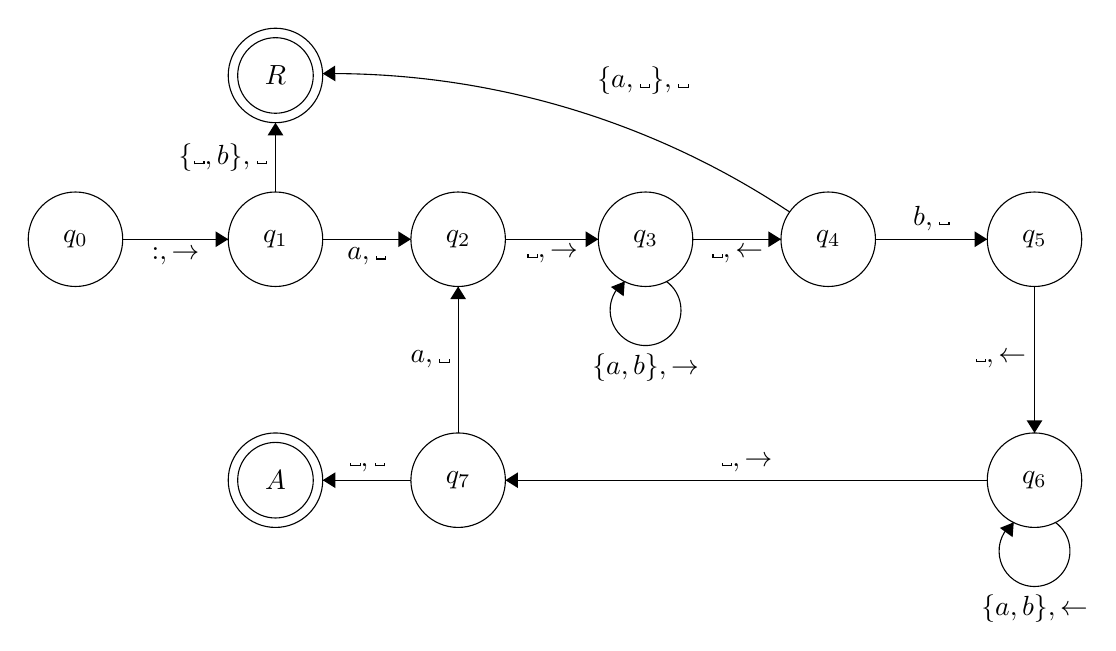
\begin{tikzpicture}[scale=0.2]
\tikzstyle{every node}+=[inner sep=0pt]
\draw [black] (7.5,-14) circle (3);
\draw (7.5,-14) node {$q_0$};
\draw [black] (20.2,-14) circle (3);
\draw (20.2,-14) node {$q_1$};
\draw [black] (20.2,-3.6) circle (3);
\draw (20.2,-3.6) node {$R$};
\draw [black] (20.2,-3.6) circle (2.4);
\draw [black] (31.8,-14) circle (3);
\draw (31.8,-14) node {$q_2$};
\draw [black] (43.7,-14) circle (3);
\draw (43.7,-14) node {$q_3$};
\draw [black] (55.3,-14) circle (3);
\draw (55.3,-14) node {$q_4$};
\draw [black] (68.4,-14) circle (3);
\draw (68.4,-14) node {$q_5$};
\draw [black] (68.4,-29.3) circle (3);
\draw (68.4,-29.3) node {$q_6$};
\draw [black] (20.2,-29.3) circle (3);
\draw (20.2,-29.3) node {$A$};
\draw [black] (20.2,-29.3) circle (2.4);
\draw [black] (31.8,-29.3) circle (3);
\draw (31.8,-29.3) node {$q_7$};
\draw [black] (10.5,-14) -- (17.2,-14);
\fill [black] (17.2,-14) -- (16.4,-13.5) -- (16.4,-14.5);
\draw (13.85,-14.5) node [below] {$:,\rightarrow$};
\draw [black] (20.2,-11) -- (20.2,-6.6);
\fill [black] (20.2,-6.6) -- (19.7,-7.4) -- (20.7,-7.4);
\draw (19.7,-8.8) node [left] {$\{\tvs,b\},\tvs$};
\draw [black] (23.2,-14) -- (28.8,-14);
\fill [black] (28.8,-14) -- (28,-13.5) -- (28,-14.5);
\draw (26,-14.5) node [below] {$a,\tvs$};
\draw [black] (34.8,-14) -- (40.7,-14);
\fill [black] (40.7,-14) -- (39.9,-13.5) -- (39.9,-14.5);
\draw (37.75,-14.5) node [below] {$\tvs,\rightarrow$};
\draw [black] (46.7,-14) -- (52.3,-14);
\fill [black] (52.3,-14) -- (51.5,-13.5) -- (51.5,-14.5);
\draw (49.5,-14.5) node [below] {$\tvs,\leftarrow$};
\draw [black] (23.197,-3.482) arc (90.62681:56.36446:52.499);
\fill [black] (23.2,-3.48) -- (24,-3.97) -- (23.99,-2.97);
\draw (43.54,-4.85) node [above] {$\{a,\tvs\},\tvs$};
\draw [black] (45.023,-16.68) arc (54:-234:2.25);
\draw (43.7,-21.25) node [below] {$\{a,b\},\rightarrow$};
\fill [black] (42.38,-16.68) -- (41.5,-17.03) -- (42.31,-17.62);
\draw [black] (58.3,-14) -- (65.4,-14);
\fill [black] (65.4,-14) -- (64.6,-13.5) -- (64.6,-14.5);
\draw (61.85,-13.5) node [above] {$b,\tvs$};
\draw [black] (68.4,-17) -- (68.4,-26.3);
\fill [black] (68.4,-26.3) -- (68.9,-25.5) -- (67.9,-25.5);
\draw (67.9,-21.65) node [left] {$\tvs,\leftarrow$};
\draw [black] (65.4,-29.3) -- (34.8,-29.3);
\fill [black] (34.8,-29.3) -- (35.6,-29.8) -- (35.6,-28.8);
\draw (50.1,-28.8) node [above] {$\tvs,\rightarrow$};
\draw [black] (69.723,-31.98) arc (54:-234:2.25);
\draw (68.4,-36.55) node [below] {$\{a,b\},\leftarrow$};
\fill [black] (67.08,-31.98) -- (66.2,-32.33) -- (67.01,-32.92);
\draw [black] (31.8,-26.3) -- (31.8,-17);
\fill [black] (31.8,-17) -- (31.3,-17.8) -- (32.3,-17.8);
\draw (31.3,-21.65) node [left] {$a,\tvs$};
\draw [black] (28.8,-29.3) -- (23.2,-29.3);
\fill [black] (23.2,-29.3) -- (24,-29.8) -- (24,-28.8);
\draw (26,-28.8) node [above] {$\tvs,\tvs$};
\end{tikzpicture}
\end{center}

\end{comment}

\begin{Q}
\mbox{}
\begin{enumerate}[a)]
\item Give an example of a formal language that is r.e. but not recursive.
\item Give an example of a formal language that is not r.e.
\end{enumerate}
\end{Q}
\begin{comment}
\textbf{Solution}
\begin{enumerate}[a)]
\item SA (see Definition \ref{D:SA}).
\item NSA (see Definition \ref{D:NSA}). 
\end{enumerate}
\end{comment}


\begin{Q}
\mbox{}
\begin{enumerate}[a)]
\item Prove that if a language $L$ and its complement $\bar{L}$ are both r.e. then $L$ is actually recursive.
\item Let $L$ be the language containing (in encoded form) all pairs $(M, w)$ such that $M$ is a Turing machine and $w$ is a string such that $M$ does \emph{not} halt on input $w$. Prove that $L$ is not r.e. HINT: Think about the halting problem and part a).   
\end{enumerate}
\end{Q}
\begin{comment}
\textbf{Solution}
\begin{enumerate}[a)]
\item Theorem \ref{T:comps}
\item Let $L'$ be the language consisting of $L$ together with all the finite strings which are not the coded form of a Turing machine and an input. Since it is decidable whether a string is the coded form of a Turing machine and an input (by the definition of encoding), $L'$ is r.e. if and only if $L$ is r.e. Note that $L'$ is the complement of the language consisting of the codes of $(T,I)$ such that $T(I)$ halts. This is the Halting problem, which we know is semidecidable but not decidable. Since the Halting problem is semidecidable, if $L'$ were r.e. then the Halting problem would be decidable, by part a). Since this is false, $L'$ and thus $L$ cannot be r.e.
\end{enumerate}
\end{comment}



\begin{Q}
Let $P$ be a property of finite strings over some fixed finite alphabet $\Sigma$ such that $P$ is true for least one finite string $s\in\Sigma^*$ (i.e. $P(s)$ holds). Let $D$ be the following decision problem: 

``Given a Turing machine $T$, does $T$ halt for every input $I$ such that $P(I)$ holds?"'.

Prove that $D$ is undecidable. HINT: prove $ETHP\leq D$.
\end{Q}
\begin{comment}
\textbf{Solution}
Let $T$ be a Turing machine (an instance of ETHP). Define the machine $M_T$ that operates as follows:
\begin{enumerate}
\item $M_T$ erases the input.
\item $M_T$ computes $T(\varepsilon)$.
\end{enumerate}
Since $M_T$ is a Turing machine, it is an instance of $D$. We need to show that the reduction is correct.
\begin{itemize}
\item Suppose $T(\varepsilon)$ halts. Then $M_T(I)$ halts for all $I$, so it certainly halts for all $I$ such that $P(I)$ holds. I.e. a yes instance of ETHP becomes a yes instance of $D$.
\item Conversely, suppose $T(\varepsilon)$ does not halt. Then, in particular, if $s\in\Sigma^*$ is chosen so that $P(s)$ holds, we have that $M_T(s)$ does not halt. I.e. a no instance of ETHP becomes a no instance of $D$. 
\end{itemize}
\end{comment}

\begin{Q}
\mbox{}
\begin{enumerate}[a)]
\item Let $k\in\bbN\setminus\{0\}$, and let $f:\bbR\to\bbR$ be a non-negative valued function (i.e. $f(x)\geq 0$ for all $x$). Show that $O(f(n))=O(kf(n))$. I.e. if $g$ is $O(f(n))$ then $g$ is also $O(kf(n))$, and vice versa.
\item Let $f,h:\bbR\to\bbR$ be non-negative valued functions, and suppose that there is $x_0\in\bbR$ such that $f(x)\leq h(x)$ for all $x\geq x_0$. Show that $O(f(n)+h(n))= O(h(n))$. I.e. if $g$ is $O(f(n)+h(n))$ then $g$ is also $O(h(n))$, and vice versa.
\end{enumerate}
\end{Q}
\begin{comment}
\textbf{Solution}
\begin{enumerate}[a)]
\item If $g$ is $O(f(n))$ there is a constant $c$ with $|g(n)|\leq cf(n)$ for large $n$. Clearly $|g(n)|\leq ckf(n)$ too, so $g$ is $O(kf(n))$. Conversely, if $g$ is $O(kf(n))$ there is a constant $c$ with $|g(n)|\leq ckf(n)$ for large $n$. But then $g$ is also $O(f(n))$ as we can use $ck$ for the constant. 
\item If $g$ is $O(f(n)+h(n))$ there is $c$ with $|g(n)|\leq c(f(n)+h(n))$ for all large $n$. By assumption, for large enough $n$ we also have $f(n)\leq h(n)$, so for values of $n$ that are `large' by both measures we have $|g(n)|\leq c(f(n)+h(n)) \leq 2ch(n)$. So $g$ is also $O(h(n))$, using the constant value $2c$. Conversely, if $|g(n)|\leq cf(n)$, then $|g(n)|\leq c(f(n)+h(n))$, as $f$ and $h$ are non-negative valued. So if $g$ is $O(h(n))$ it is also $O(f(n)+h(n))$. 
\end{enumerate}
\end{comment}


\begin{Q}
Recall Definition \ref{D:TSDP}. 
\begin{enumerate}[a)]
\item Show that $TSDP$ is in $\NP$ (HINT: describe a $p$-time verifier). 
\item Assuming that $HCP$ is $\NP$-complete, prove the converse of Theorem \ref{T:TSDPtoHCP} (i.e. that $TSDP\leq_p HCP$).
\end{enumerate}
\end{Q}
\begin{comment}
\textbf{Solution}
\begin{enumerate}[a)]
\item The certificates for the verifier are (coded forms of) sequences of vertices. The verifier checks if a given certificate defines a Hamiltonian circuit with an appropriate weight. It accepts if so, and rejects otherwise.
\item $TSDP\leq_p HCP$ by $NP$-hardness of $HCP$.
\end{enumerate}
\end{comment}

\begin{Q}\mbox{}
\begin{itemize}
\item A \emph{clique} in a graph $G$ is a set $C$ of vertices of $G$ such that every pair of distinct vertices in $C$ is connected by an edge. 
\item Let CLIQUE be the decision problem ``Given a graph $G$ and $k\in \bbN$, does $G$ contain a clique of size at least $k$?".
\item An \emph{independent set} in a graph $G$ is a set of vertices $I$ of $G$ such that no pair of vertices in $I$ is connected by an edge.
\item Let INDSET be the decision problem ``Given a graph $G$ and $k\in \bbN$, does $G$ contain an independent set of size at least $k$?".   
\end{itemize}
Prove that $CLIQUE \equiv_p INDSET$.
\end{Q}
\begin{comment}
\textbf{Solution}
Given a graph $G$, define the graph $\bar{G}$ to have the same vertices as $G$, and say there is an edge $\{u,v\}$ in $\bar{G}$ if and only if there is not an edge $\{u,v\}$ in $G$. This construction clearly takes $p$-time. Moreover, a clique/independent set of size $k$ in $G$ is an independent set/clique of size $k$ in $\bar{G}$, and vice versa. So this transformation maps yes instance of CLIQUE to yes instances of INDSET, and vice versa. So $CLIQUE \leq_p INDSET$ and $INDSET\leq_p CLIQUE$. I.e. $CLIQUE \equiv_p INDSET$.  
\end{comment}

\begin{Q}
Look at the proof of the fact that $\SAT$ is $\NP$-complete (Theorem \ref{T:cook}). Using the notation given in that proof, write down a Boolean formula $\psi$ that expresses that at some point the machine is in the accept state.
\end{Q}
\begin{comment}
\textbf{Solution}
Let $A$ be the accept state. Then $\psi = \bigvee_{1\leq i,j\leq Cn^k} p_{i,j,A}$.
\end{comment}





\end{document}
\newpage
\section{Further reading}
A classic introduction can be found in \cite{Sip12}. Unfortunately I don't think this is freely distributed by the author. There's also \cite{Sav98}, which the author generously makes available under a creative commons license.  Also, if you want to draw Turing machine diagrams, this tool is great, especially if you use LaTeX: \url{http://madebyevan.com/fsm/}. 


\newpage
\includecomment{comment}
% Add label padding to avoid reference conflicts
\renewcommand*{\prefix}{PAD}

% This is a bit of a hack as I wanted to number exercise solutions with the same numbers as the original exercises, but the internal referncing does not like this at all.
% My solution is to make the subsections invisible with *. This throws a lot of warnings but the document produced is functional.
% Removing * causes these subsections to appear in the ToC (the warnings remain), but the link does not function correctly. 

\section{Appendix - Solutions to exercises}
\setcounter{section}{2}
\section*{Models of Computation}
\documentclass{article}

\usepackage{amsmath, mathrsfs, amssymb, stmaryrd, cancel, relsize,tikz,amsthm,comment,enumerate}

\theoremstyle{definition}
\newtheorem{Q}{Question}

\newcommand{\tvs}{\textvisiblespace}
\newcommand{\ra}{\rightarrow}
\newcommand{\la}{\leftarrow}
%\includecomment{comment}

%\pagenumbering{gobble}

\title{ITCS 532 Foundations of Computer Science\\
Week 1 - Models of Computation (Homework)}
\author{Rob Egrot}
\date{}

\begin{document}
\maketitle

\begin{Q}
A quadratic in $x$ over the integers has form $q(x)=ax^2+bx+c$, where $x$ is a variable and $a,b$ and $c$ are integers. Suppose our decision problem is whether a given quadratic over the integers has a root in the integers. So the set of instances is the set of all quadratics over the integers. A quadratic $q$ is a yes instance if there is an integer $z$ such that $q(z)=0$.

Design a suitable encoding system for this decision problem (you don't need to design a Turing machine to solve it!).
\end{Q}
\begin{comment}
\textbf{Solution}
Use $\Sigma = \{1,-,*\}$. Store $a$, $b$ and $c$ in unary, separated by $*$, using $-$ to denote negatives. E.g. we express $2x^2 - 3x +1$ as $11*-111*1$.
\end{comment}

\begin{Q}
Let $\Sigma=\{1,*\}$. Design a Turing machine that accepts as input a unary number (i.e. a finite string containing only 1s), and outputs that number multiplied by 2. E.g. If the input is 111 the output will be 111111. Hint: $*$ does not appear in the input or the output, but we can use it during the process of calculating the output.
\end{Q}
\begin{comment}
\textbf{Solution}
\begin{center}
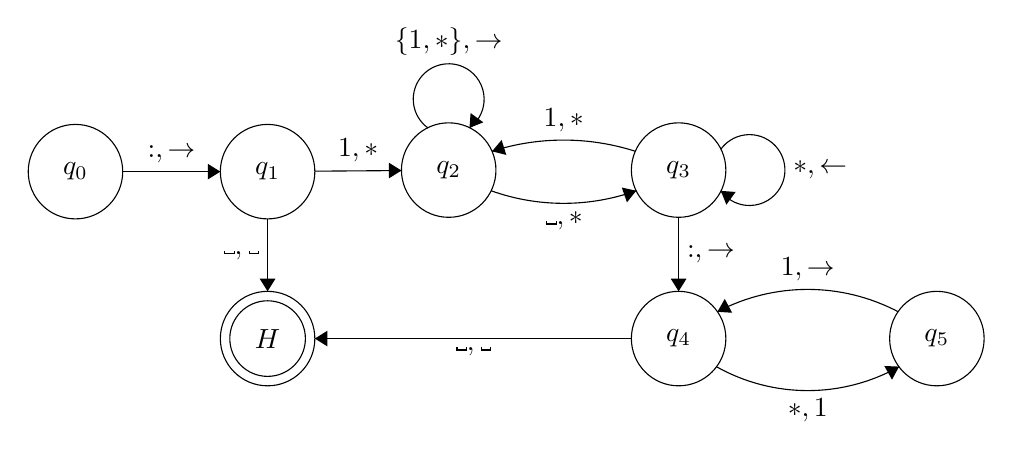
\begin{tikzpicture}[scale=0.2]
\tikzstyle{every node}+=[inner sep=0pt]
\draw [black] (14.6,-15.2) circle (3);
\draw (14.6,-15.2) node {$q_0$};
\draw [black] (26.8,-15.2) circle (3);
\draw (26.8,-15.2) node {$q_1$};
\draw [black] (26.8,-25.8) circle (3);
\draw (26.8,-25.8) node {$H$};
\draw [black] (26.8,-25.8) circle (2.4);
\draw [black] (38.3,-15.1) circle (3);
\draw (38.3,-15.1) node {$q_2$};
\draw [black] (52.9,-15.1) circle (3);
\draw (52.9,-15.1) node {$q_3$};
\draw [black] (52.9,-25.8) circle (3);
\draw (52.9,-25.8) node {$q_4$};
\draw [black] (69.3,-25.8) circle (3);
\draw (69.3,-25.8) node {$q_5$};
\draw [black] (17.6,-15.2) -- (23.8,-15.2);
\fill [black] (23.8,-15.2) -- (23,-14.7) -- (23,-15.7);
\draw (20.7,-14.7) node [above] {$:,\ra$};
\draw [black] (26.8,-18.2) -- (26.8,-22.8);
\fill [black] (26.8,-22.8) -- (27.3,-22) -- (26.3,-22);
\draw (26.3,-20.5) node [left] {$\tvs,\tvs$};
\draw [black] (29.8,-15.17) -- (35.3,-15.13);
\fill [black] (35.3,-15.13) -- (34.5,-14.63) -- (34.5,-15.63);
\draw (32.55,-14.63) node [above] {$1,\ast$};
\draw [black] (36.977,-12.42) arc (234:-54:2.25);
\draw (38.3,-7.85) node [above] {$\{1,\ast\},\ra$};
\fill [black] (39.62,-12.42) -- (40.5,-12.07) -- (39.69,-11.48);
\draw [black] (50.209,-16.412) arc (-70.28917:-109.71083:13.666);
\fill [black] (50.21,-16.41) -- (49.29,-16.21) -- (49.62,-17.15);
\draw (45.6,-17.71) node [below] {$\tvs,\ast$};
\draw [black] (55.58,-13.777) arc (144:-144:2.25);
\draw (60.15,-15.1) node [right] {$\ast,\la$};
\fill [black] (55.58,-16.42) -- (55.93,-17.3) -- (56.52,-16.49);
\draw [black] (52.9,-18.1) -- (52.9,-22.8);
\fill [black] (52.9,-22.8) -- (53.4,-22) -- (52.4,-22);
\draw (53.4,-20.45) node [right] {$:,\ra$};
\draw [black] (66.899,-27.585) arc (-60.64203:-119.35797:11.828);
\fill [black] (66.9,-27.58) -- (65.96,-27.54) -- (66.45,-28.41);
\draw (61.1,-29.6) node [below] {$\ast,1$};
\draw [black] (55.359,-24.095) arc (117.75844:62.24156:12.326);
\fill [black] (55.36,-24.1) -- (56.3,-24.16) -- (55.83,-23.28);
\draw (61.1,-22.18) node [above] {$1,\ra$};
\draw [black] (49.9,-25.8) -- (29.8,-25.8);
\fill [black] (29.8,-25.8) -- (30.6,-26.3) -- (30.6,-25.3);
\draw (39.85,-26.3) node [below] {$\tvs,\tvs$};
\draw [black] (41.046,-13.906) arc (107.74904:72.25096:14.937);
\fill [black] (41.05,-13.91) -- (41.96,-14.14) -- (41.66,-13.19);
\draw (45.6,-12.69) node [above] {$1,\ast$};
\end{tikzpicture}
\end{center}
\end{comment}

\begin{Q}
Can a formal language $L$ exist that is recursive but not r.e.?
\end{Q}
\begin{comment}
\textbf{Solution}
No. We know from the notes that decidable implies semidecidable, and this is just the formal language version of that.
\end{comment}

\begin{Q}
Suppose we define a class $\mathcal C$ of abstract computational devices similar to Turing machines but without the $\la$ command (so the tape head may never move backwards).
\begin{enumerate}[(a)]
\item Give an informal argument for why this model of computation is strictly weaker than that of Turing machines.
\item Would it make any difference if we replaced the $\la$ command with a $-$ command that keeps the tape head in the same place?
\item (Hard) Give a rigorous proof for part (a).
\end{enumerate}
\end{Q}
\begin{comment}
\textbf{Solution}
\begin{enumerate}[(a)]
\item No memory.
\item No. Still no memory. 
\item Consider the problem of checking to see if two strings are the same length. Input is, for example, a string of $1$'s followed by a $*$, followed by another string of $1$'s. Suppose we have a $-$ machine $M$ that solves this problem. Then it has a finite number of states, $n$ say. Consider the set $X$ that contains all strings of $k$ ones followed by a $*$, for $k\in\{1,\ldots,n+1\}$. Since $M$ cannot move its tape head backwards, the state it's in when it gets to the $*$ symbol must store all the information about the length of the first string. As $|X| = n+1$, by the pigeon hole principle there must be (at least) two strings in $X$ such that $M$ is in the same state when it gets to $*$. Call these strings $s*$ and $t*$. Then $M$ should accept $s*s$, but then it must also accept $t*s$, which is incorrect. 
\end{enumerate}
\end{comment}

\end{document}

\section*{Turing Machine Variants}
\setcounter{section}{3}
\setcounter{Q}{0}
\documentclass{article}

\usepackage{amsmath, mathrsfs, amssymb, stmaryrd, cancel, relsize,tikz,amsthm,comment,enumerate}

\theoremstyle{definition}
\newtheorem{Q}{Question}

\newcommand{\tvs}{\textvisiblespace}
\newcommand{\ra}{\rightarrow}
\newcommand{\la}{\leftarrow}
\newcommand{\bbN}{\mathbb{N}}

%\includecomment{comment}


\title{ITCS 532 Foundations of Computer Science\\
Week 2 - Turing Machine Variants (Homework)}
\author{Rob Egrot}
\date{}

\begin{document}
\maketitle

\begin{Q}
Let $\Sigma=\{a,b,c\}$. Let $L$ be the set of all finite strings containing the substring $ab$. Design a Turing machine that decides $L$. What regular expression describes $L$?
\end{Q}
\begin{comment}
\textbf{Solution}
\begin{center}
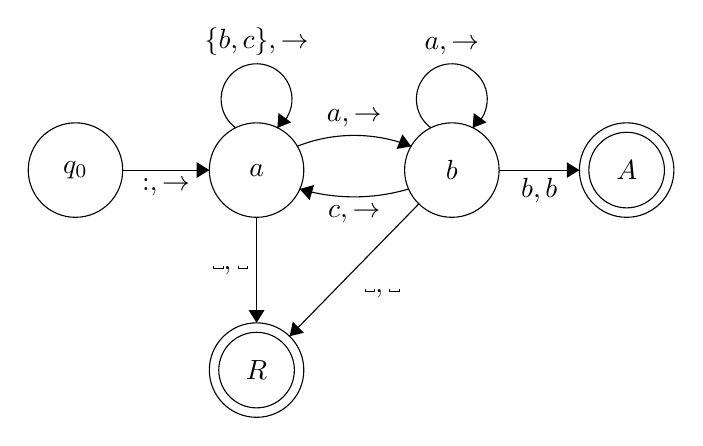
\begin{tikzpicture}[scale=0.2]
\tikzstyle{every node}+=[inner sep=0pt]
\draw [black] (15.4,-24.4) circle (3);
\draw (15.4,-24.4) node {$q_0$};
\draw [black] (26.9,-24.4) circle (3);
\draw (26.9,-24.4) node {$a$};
\draw [black] (39.3,-24.4) circle (3);
\draw (39.3,-24.4) node {$b$};
\draw [black] (50.4,-24.4) circle (3);
\draw (50.4,-24.4) node {$A$};
\draw [black] (50.4,-24.4) circle (2.4);
\draw [black] (26.9,-37.1) circle (3);
\draw (26.9,-37.1) node {$R$};
\draw [black] (26.9,-37.1) circle (2.4);
\draw [black] (18.4,-24.4) -- (23.9,-24.4);
\fill [black] (23.9,-24.4) -- (23.1,-23.9) -- (23.1,-24.9);
\draw (21.15,-24.9) node [below] {$:,\ra$};
\draw [black] (29.478,-22.889) arc (111.61948:68.38052:9.829);
\fill [black] (36.72,-22.89) -- (36.16,-22.13) -- (35.79,-23.06);
\draw (33.1,-21.7) node [above] {$a,\ra$};
\draw [black] (25.577,-21.72) arc (234:-54:2.25);
\draw (26.9,-17.15) node [above] {$\{b,c\},\ra$};
\fill [black] (28.22,-21.72) -- (29.1,-21.37) -- (28.29,-20.78);
\draw [black] (26.9,-27.4) -- (26.9,-34.1);
\fill [black] (26.9,-34.1) -- (27.4,-33.3) -- (26.4,-33.3);
\draw (26.4,-30.75) node [left] {$\tvs,\tvs$};
\draw [black] (37.2,-26.55) -- (29,-34.95);
\fill [black] (29,-34.95) -- (29.91,-34.73) -- (29.2,-34.03);
\draw (33.63,-32.22) node [right] {$\tvs,\tvs$};
\draw [black] (42.3,-24.4) -- (47.4,-24.4);
\fill [black] (47.4,-24.4) -- (46.6,-23.9) -- (46.6,-24.9);
\draw (44.85,-24.9) node [below] {$b,b$};
\draw [black] (37.977,-21.72) arc (234:-54:2.25);
\draw (39.3,-17.15) node [above] {$a,\ra$};
\fill [black] (40.62,-21.72) -- (41.5,-21.37) -- (40.69,-20.78);
\draw [black] (36.558,-25.599) arc (-73.45716:-106.54284:12.146);
\fill [black] (29.64,-25.6) -- (30.27,-26.31) -- (30.55,-25.35);
\draw (33.1,-26.6) node [below] {$c,\ra$};
\end{tikzpicture}
\end{center}

The regular expression is $\cdot ab \cdot$ if we treat the alphabet as implicit, or, if we want to specify the alphabet, we could use $(a|b|c)^\ast ab (a|b|c)^\ast$ .
\end{comment}

\begin{Q}
Let $\Sigma$ be a finite alphabet. Consider the class $\mathcal C$ of Turing machine variants over $\Sigma$ with a countably infinite number of tape heads instead of only one. So the transition function is defined by \begin{equation*}\delta:(Q\setminus H)\times \Sigma^\omega \to Q\times(\Sigma\setminus\{:\}\cup \{\la,\ra\})^\omega \end{equation*}
Let $L\subseteq \Sigma^*$ be any language over $\Sigma$. Show that there is a machine in $\mathcal C$ that decides $L$. What does this tell us about the relative power of $\mathcal C$ and the class of regular Turing machines?

HINT: To make this question easier, you can assume that the machine can tell when different tape heads are reading the same space on the tape, and that this information can be used by the transition function. If you want an extra-difficult challenge try to do without this assumption.
\end{Q}
\begin{comment}
\textbf{Solution}
With the assumption: The machine operates as follows:
\begin{enumerate}
\item Move all the tape heads to the right, so they are all reading the first symbol on the tape.
\item Move all tape heads except the first to the right, so the first is still reading the first symbol, and the rest are reading the second symbol. 
\item Move all except the first and second tape head to the right.
\item Keep following this pattern till the first blank space is found.
\item Now there are $n$ tape heads reading the $n$ characters of the input string, and the rest of the tape heads are all reading a blank space.
\item Write the transition function so that if the string being read is in $L$ the machine accepts, and it rejects otherwise.
\end{enumerate}
The assumption is used here so the machine knows which tape heads to move at each step. E.g. if heads 4 and 5 are reading the same space but heads 3 and 4 are not, it can use this information to say that head 4 must stay in place and all higher numbered heads must move right.
\newline
\newline 
This tells us this new kind of machine is much more powerful than regular Turing machines. 
\newline
\newline
Without the assumption: Let the tape heads be $h_1,h_2,\ldots$. The machine operates as follows:
\begin{itemize}
\item (Step 0) Move all the tape heads to the right, so they are all reading the first symbol on the tape.
\item (Step 1) Move all the tape heads $h_i$ such that $2|i$ to the right, and keep the others in place, except for $h_1$ which moves back to the start of the tape.
\item (Step 2) Move all the tape heads $h_i$ such that $2$ and $3$ divide $i$ to the right. Keep the others in place except $h_1$ which moves back to square 1 (as it must do this), and also move $h_3$ back to the start of the tape.
\item (Step 3) Move all the tape heads $h_i$ such that $i$ is divisible by $2,3,5$ to the right. Keep the others in place except $h_3$ which moves back to square 1, and also move $h_5$ back to the start of the tape.
\item (Step 4) Move the tape heads $h_i$ such that $i$ is divisible by $2,3,5,7$ to the right. Keep the others in place except $h_5$ which moves back to square 1, and also move $h_7$ back to the start of the tape.
\item (Step $k$) To understand the pattern here we list the prime numbers (in order) as $p_1,p_2,\ldots$. At the start of computation step $k>2$, the tape heads with numbers divisible by $p_1\times\ldots \times p_{k-1}$ are reading cell $k-1$. The head $h_{p_{k-1}}$ is also back at the start of the tape reading the $:$ symbol. The fact that $h_{p_{k-1}}$ is reading $:$ is very important, as using this we can code the machine so that it advances all tape heads with numbers divisible by $p_1\times\ldots \times p_{k}$ to the right, and also send head $h_{p_k}$ back ready for the next round.
\item At some point there will be an infinite number of tape heads reading the blank space symbol. This tells the machine the end of the input has been reached.
\item When the end has been reached, we have an infinite set of tape heads reading the first symbol of the input, another infinite set reading the 2nd symbol, and so on. Moreover, these infinite sets are distinguishable by the numbers of the heads they contain (e.g. the first contains odd numbered heads, the second contains those divisible by 2, but not by any other prime, and so on). We write the transition function so that if the string being read is in $L$ the machine accepts, and it rejects otherwise.
\end{itemize}
\end{comment}

The next questions are to revise the concept of countable and uncountable sets, because we'll need them later. You may find it useful to review the class on cardinal numbers from the 531 course.

\begin{Q}
Let $\Sigma$ be a finite alphabet. Prove that $\Sigma^*$ is countably infinite. 
\end{Q}
\begin{comment}
\textbf{Solution}
$\Sigma^*$ is the set of all finite strings using $\Sigma$, so is obviously infinite. To prove it is countable it is sufficient to find a 1-1 function $f:\Sigma^*\to \bbN$. We construct an example of a function like this. Suppose $\Sigma = \{\sigma_1,\ldots,\sigma_n\}$. Let $p_1,p_2,p_3,\ldots$ list the prime numbers in ascending order. Given a string $s = \sigma_{i_1}\sigma_{i_2}\ldots\sigma_{i_k}$, define $f(s) = p_1^{i_1}\times p_2^{i_2}\times \ldots \times p_k^{i_k}$. 

So, for example, if the alphabet is $\{ a = \sigma_0, b = \sigma_1, c=\sigma_2\}$, the string $aacb$ corresponds to $2^13^15^37^2$. I.e., the letter $a$ is at positions 1 and 2 (corresponding to $p_1 = 2$ and $p_2 = 3$, the 1st and 2nd primes), the letter $c$ is at position 3, and the letter $b$ is at position 4. 

Then $f$ is 1-1 because, by the Fundamental Theorem of Arithmetic, numbers are specified uniquely by their prime factorizations (up to reordering).
\end{comment}

\begin{Q}
Let $\Sigma$ again be a finite alphabet. Is $\wp(\Sigma^*)$ countable? Justify your answer.
\end{Q}
\begin{comment}
\textbf{Solution}
This must be uncountable so long as $\Sigma$ is non-empty, because, as proved in the notes for the 531 course, given a non-empty set $X$ we always have $|X|<|\wp(X)|$. 
\end{comment}

\begin{Q}
Recall that the union of a countable number of countable sets is countable. Let $\Sigma=\{0,1\}$ and let $X=\wp(\Sigma^*)$ be the uncountable set of all languages over $\Sigma$. Let $C_1$ and $C_2$ be countable subsets of $X$, and let $U$ be an uncountable subset of $X$. Remember that if $Y$ is a set we use $\bar{Y}$ to denote the complement of $Y$. For each of the following sets say whether it is countable, uncountable, or dependent on the choice of $C_1,C_2,U$. Justify your answers.
\begin{enumerate}[(a)]
\item$C_1\cup C_2$
\item$\bar{C_1}$
\item$\bar{U}$
\item$\bar{C_1}\cap U$
\end{enumerate} 
\end{Q}
\begin{comment}
\textbf{Solution}
\begin{enumerate}[(a)]
\item This is countable as the union of a countable number of countable sets is always countable.
\item This must be uncountable, as $C_1\cup \bar{C}_1 = X$. By part (a), if both $C_1$ and $\bar{C}_1$ were countable then $X$ would be too, but $X$ is uncountable. So, since $C_1$ is countable, $\bar{C}_1$ must be uncountable.
\item This depends on the choice of $U$. If $U = X$ then $\bar{U} = \emptyset$, which is countable. Alternatively, let $U$ be the set of all languages containing the string $s$, for some arbitrary choice of $s$. Then $U$ is in bijection with $\wp(\Sigma^*\setminus\{s\})$, which is uncountable for the same reason $\wp(\Sigma^*)$ is. This bijection takes a language $L\in U$ to $L\setminus\{s\}$, which is in $\wp(\Sigma^*\setminus\{s\})$, and conversely takes $L'\in\wp(\Sigma^*\setminus\{s\})$ to $L'\cup\{s\}$, which is in $U$. Moreover, $\bar{U} = \wp(\Sigma^*\setminus\{s\})$, and so is also uncountable.   
\item This is uncountable, for the following reason.
\begin{align*}
U &= X \cap U \\
&=(\bar{C}_1\cup C_1)\cap U \\
&= (\bar{C}_1 \cap U) \cup (C_1\cap U).
\end{align*}
Now, $(C_1\cap U)$ is countable, so $(\bar{C}_1 \cap U)$ must be uncountable as $U$ is. This last step is essentially the same argument we used in part (b).
\end{enumerate}
\end{comment}



\end{document}

\section*{Universal Turing Machines}
\setcounter{section}{4}
\setcounter{Q}{0}
\documentclass{article}

\usepackage{amsmath, mathrsfs, amssymb, stmaryrd, cancel, relsize,tikz,amsthm,comment,graphicx}

\theoremstyle{definition}
\newtheorem{Q}{Question}

\newcommand{\tvs}{\textvisiblespace}
\newcommand{\ra}{\rightarrow}
\newcommand{\la}{\leftarrow}
\newcommand{\co}{\mathbf{code}}

%\includecomment{comment}

% uncomment below to allow file to build as a stand-alone document
% this is part of a hack to allow the same file to be input twice without mixing up labels when building main document
%\renewcommand{\prefix}{}

\title{ITCS 532 Foundations of Computer Science\\
Week 3 - Universal Turing Machines (Homework)}
\author{Rob Egrot}
\date{}

\begin{document}
\maketitle

\begin{Q}\label{\prefix Q:T}
Consider the following Turing machine $T$ over alphabet $\{a\}$.

\begin{center}
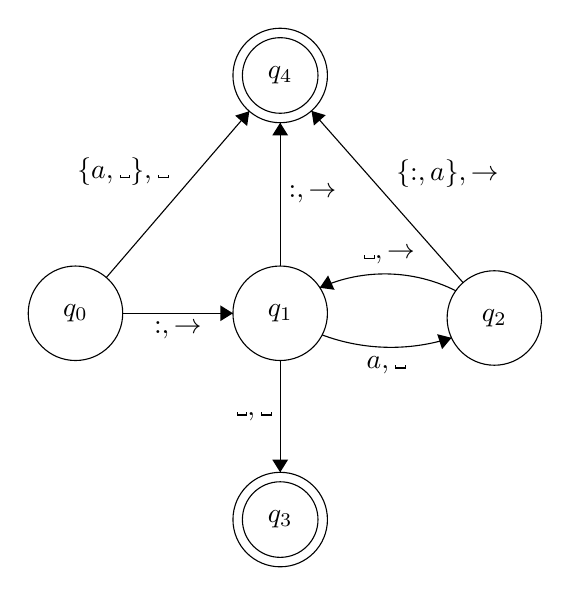
\begin{tikzpicture}[scale=0.2]
\tikzstyle{every node}+=[inner sep=0pt]
\draw [black] (9.4,-31.3) circle (3);
\draw (9.4,-31.3) node {$q_0$};
\draw [black] (22.4,-31.3) circle (3);
\draw (22.4,-31.3) node {$q_1$};
\draw [black] (36,-31.6) circle (3);
\draw (36,-31.6) node {$q_2$};
\draw [black] (22.4,-44.4) circle (3);
\draw (22.4,-44.4) node {$q_3$};
\draw [black] (22.4,-44.4) circle (2.4);
\draw [black] (22.4,-16.2) circle (3);
\draw (22.4,-16.2) node {$q_4$};
\draw [black] (22.4,-16.2) circle (2.4);
\draw [black] (12.4,-31.3) -- (19.4,-31.3);
\fill [black] (19.4,-31.3) -- (18.6,-30.8) -- (18.6,-31.8);
\draw (15.9,-31.8) node [below] {$:,\ra$};
\draw [black] (11.36,-29.03) -- (20.44,-18.47);
\fill [black] (20.44,-18.47) -- (19.54,-18.75) -- (20.3,-19.41);
\draw (15.35,-22.3) node [left] {$\{a,\tvs\},\tvs$};
\draw [black] (33.284,-32.856) arc (-72.05443:-110.47292:12.503);
\fill [black] (33.28,-32.86) -- (32.37,-32.63) -- (32.68,-33.58);
\draw (29.13,-34.02) node [below] {$a,\tvs$};
\draw [black] (24.914,-29.684) arc (114.19527:63.27739:10.059);
\fill [black] (24.91,-29.68) -- (25.85,-29.81) -- (25.44,-28.9);
\draw (29.29,-28.23) node [above] {$\tvs,\ra$};
\draw [black] (22.4,-34.3) -- (22.4,-41.4);
\fill [black] (22.4,-41.4) -- (22.9,-40.6) -- (21.9,-40.6);
\draw (21.9,-37.85) node [left] {$\tvs,\tvs$};
\draw [black] (34.01,-29.35) -- (24.39,-18.45);
\fill [black] (24.39,-18.45) -- (24.54,-19.38) -- (25.29,-18.72);
\draw (29.74,-22.45) node [right] {$\{:,a\},\ra$};
\draw [black] (22.4,-28.3) -- (22.4,-19.2);
\fill [black] (22.4,-19.2) -- (21.9,-20) -- (22.9,-20);
\draw (22.9,-23.75) node [right] {$:,\ra$};
\end{tikzpicture}
\end{center}

What does $T$ do? 

\end{Q}
\begin{comment}
\textbf{Solution}
$T$ erases its input.
\end{comment}

\begin{Q}\label{\prefix Q:delta}
Write out the transition function $\delta$ for $T$ from question \ref{Q:T} in terms of tuples (i.e. $(q,\sigma,q',\sigma'))$.
\end{Q}
\begin{comment}
\textbf{Solution}
\begin{itemize}
\item $(q_0, :, q_1, \ra) = (q_0,\sigma_0,q_1,\sigma_3)$.
\item $(q_0, \tvs, q_4, \tvs) = (q_0,\sigma_1,q_4,\sigma_1)$.
\item $(q_0,a,q_4,\tvs) = (q_0, \sigma_4,q_4,\sigma_1)$.
\item $(q_1, :, q_4, \ra)= (q_1,\sigma_0,q_4,\sigma_3)$.
\item $(q_1,\tvs,q_3,\tvs) = (q_1,\sigma_1,q_3,\sigma_1)$.
\item $(q_1,a,q_2,\tvs) = (q_1,\sigma_4,q_2,\sigma_1)$.
\item $(q_2,:,q_4,\ra) = (q_2,\sigma_0,q_4,\sigma_3)$.
\item $(q_2,\tvs,q_1,\ra) = (q_2,\sigma_1,q_1,\sigma_3)$.
\item $(q_2,a,q_4,\ra) = (q_2,\sigma_4, q_4,\sigma_3)$.
\end{itemize}
\end{comment}

\begin{Q}
Let $T$ be as in question \ref{Q:T}. Using the encoding system from the notes we map every symbol from the alphabet of $T$ to some symbol in $\{\sigma_0,\sigma_1,\ldots\}$. Since $\sigma_0$, $\sigma_1$, $\sigma_2$, and $\sigma_3$ are taken by $:$, $\tvs$, $\la$ and $\ra$ respectively we let $a=\sigma_4$. Using the system from the notes and your transition function from question \ref{Q:delta} write down $\co(T)$.
\end{Q}
\begin{comment}
\textbf{Solution}\\
Assuming tuples in the same order as in the solution above (which is essentially arbitrary - if we were designing a real encoding scheme we would want to use something more principled than this):\\
 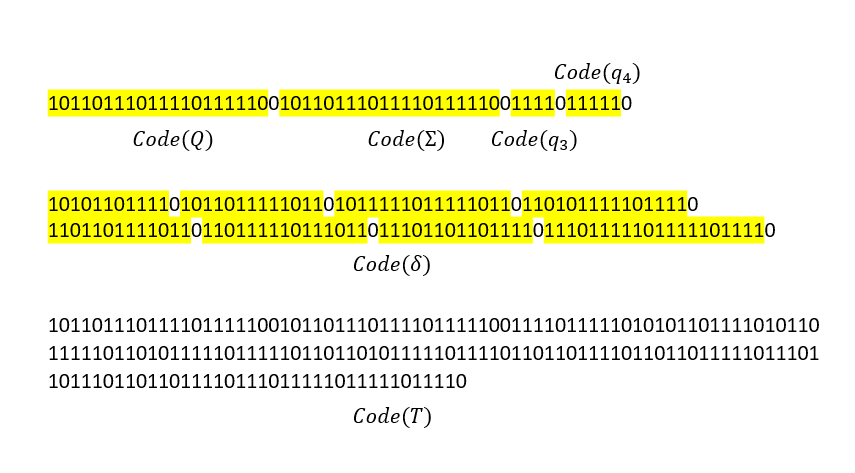
\includegraphics[width=\linewidth]{code.png}
\end{comment}

\begin{Q}
Suppose $T$ is a Turing machine over the alphabet $\{0,1,*\}$ that takes as input two binary numbers separated by $*$ and outputs their sum (in binary). Describe a way we could use $T$ to construct a Turing machine that takes as input two positive binary numbers separated by $*$ and outputs their product. You can use multiple tapes. You don't need to draw a state change diagram.
\end{Q}
\begin{comment}
\textbf{Solution}\\
\begin{enumerate}
\item Copy first number to tape 2.
\item Copy second number to tape 3. 
\item Trim tape 1 so it just contains first number.
\item If tape 3 is empty then erase tape 1 and halt.
\item If the number on tape 3 is one then halt.
\item Add number on tape 2 to the number on tape 1, then decrease number on tape 3 by one (we use $T$ in this step).
\item Go to step 5).
\end{enumerate}

We can assume we have an extra tape for side calculations if we like. We could also check to see if the first number is zero before step 6. Otherwise the machine may add zero to itself several times. This will get the right answer, but is obviously inefficient. 
\end{comment}



\end{document}

\section*{Undecidable Problems}
\setcounter{section}{5}
\setcounter{Q}{0}
\documentclass{article}

\usepackage{amsmath, mathrsfs, amssymb, stmaryrd, cancel, relsize,tikz,amsthm,comment,enumerate}

\theoremstyle{definition}
\newtheorem{Q}{Question}

\newcommand{\tvs}{\textvisiblespace}
\newcommand{\ra}{\rightarrow}
\newcommand{\la}{\leftarrow}
\newcommand{\co}{\mathbf{code}}


\title{ITCS 532 Foundations of Computer Science\\
Week 4 - Undecidable Problems (Homework)}
\author{Rob Egrot}
\date{}
%\includecomment{comment}

% uncomment below to allow file to build as a stand-alone document
% this is part of a hack to allow the same file to be input twice without mixing up labels when building main document
%\renewcommand{\prefix}{}

\begin{document}
\maketitle

\begin{Q}
Let $L_1$ and $L_2$ be disjoint r.e. languages. Suppose $L_1\cup L_2$ is recursive. Prove that $L_1$ and $L_2$ are both recursive.
\end{Q}
\begin{comment}
\textbf{Solution}\\
We will describe an algorithm for deciding $L_1$. 
\begin{enumerate}
\item Given a string $x$ we can decide if $x\in L_1\cup L_2$, as this language is recursive.
\item If $x\notin L_1\cup L_2$ then $x\notin L_1$, so reject.
\item If $x\in L_1\cup L_2$ then it must be in either $L_1\setminus L_2$, or $L_2\setminus L_1$. Use dovetailing to simultaneously run the algorithms that semidecide $L_1$ and $L_2$ on $x$.
\item If $x\in L_1$ then accept.
\item If $x\in L_2$ then reject.
\end{enumerate}
We can decide $L_2$ similarly.
\end{comment}

\begin{Q}\label{\prefix Q:100}
Let $D$ be the decision problem ``Given a Turing machine $T$ and input $I$, does $T(I)$ halt within 100 steps?". Then there is an associated formal language \[L_D=\{\co(T,I):T \text{ halts on } I \text{ within 100 steps}\}\]
Which of the following is true (give reasons)?
\begin{enumerate}
\item[i)] $L_D$ is recursive.
\item[ii)] $L_D$ is r.e but not recursive.
\item[iii)] $L_D$ is not r.e.
\end{enumerate}
\end{Q}
\begin{comment}
\textbf{Solution}\\
$L_D$ is recursive. To decide $L_D$ we use a Turing machine that, given input $\co(T,I)$ simulates $T(I)$, and also maintains a counter track of the number of steps that have been simulated. If this simulation halts before the counter reaches 100 then the input is accepted. If it does not (or if the input is not in the correct format), then it rejects.
\end{comment}

\begin{Q}\label{\prefix Q:D}
Let $D$ be the decision problem ``Given a Turing machine $T$, does $T$ halt on every input $I$ within 100 steps?". What is the formal language $L_D$ associated with $D$?
\end{Q}
\begin{comment}
\textbf{Solution}\\
$\{\co(T): T$ is a Turing machine and $T(I)$ halts within 100 steps for all $I\}$.
\end{comment}

\begin{Q}
With $D$ as in question \ref{Q:D} prove that $L_D$ is recursive. 
\end{Q}
\begin{comment}
\textbf{Solution}\\
Note that $T(I)$ halts for all $I$ within 100 steps if and only if $T(I)$ halts for all $I$ of length $\leq 100$ within 100 steps, as $T$ can never read past the first 100 symbols within 100 steps. Now, the number of strings over a finite alphabet whose length is $\leq 100$ is finite, so we can check $T(I)$ for each such string $I$ using the algorithm from question \ref{Q:100}. If the answer is no for any $I$ we reject $\co(T)$, and if the answer is yes for all $I$ we accept $\co(T)$.
\end{comment}

\begin{Q}
Let $HAI$ be the decision problem ``Given $T$ does $T$ halt for all inputs?". Then an instance of $HAI$ is a Turing machine $T$. \begin{enumerate}
\item[a)] What is an instance of the Halting Problem?
\item[b)] If $M$ is a Turing machine and $I$ is an input for $M$ let $M_I$ be a machine that first erases its input then simulates $M(I)$. Show that $M(I)$ halts if and only if $M_I(J)$ halts for all inputs $J$, and $M(I)$ runs forever if and only if $M_I(J)$ runs forever for all $J$.
\item[c)] Prove that the Halting Problem reduces to $HAI$.
\item[d)] What does this tell us about the decidability of $HAI$?
\end{enumerate} 
\end{Q}
\begin{comment}
\textbf{Solution}\\
\begin{enumerate}[a)]
\item A pair $(M,I)$ where $M$ is a Turing machine and $I$ is a finite string over its alphabet.
\item By definition $M(I)$ halts if and only if $M_I(J)$ halts for all $J$. So the contrapositive statement says that $M(I)$ runs forever if and only if $M_I(J)$ runs forever for some $J$. But $M_I(J)$ does the same thing for all $J$, so $M(I)$ runs forever if and only if $M_I(J)$ runs forever for all $J$.
\item Given an instance $(M,I)$ of HP we construct an instance $M_I$ of HAI as described. We have just proved that $(M,I)$ is a yes instance of HP if and only if $M_I$ is a yes instance of HAI.
\item As $HP\leq HAI$, and $HP$ is undecidable, it follows that $HAI$ is undecidable.
\end{enumerate}
\end{comment}

\end{document}

\section*{The Entscheidungsproblem}
\setcounter{section}{6}
\setcounter{Q}{0}
\documentclass{article}

\usepackage{amsmath, mathrsfs, amssymb, stmaryrd, cancel, relsize,tikz,amsthm,comment}

\theoremstyle{definition}
\newtheorem{Q}{Question}

\newcommand{\tvs}{\textvisiblespace}
\newcommand{\ra}{\rightarrow}
\newcommand{\la}{\leftarrow}
\newcommand{\co}{\mathbf{code}}


\title{ITCS 532 Foundations of Computer Science\\
Week 5 - The Entscheidungsproblem (Homework)}
\author{Rob Egrot}
\date{}
%\includecomment{comment}
\begin{document}
\maketitle

\begin{Q}
Let $L=\{\co(T):T$ is a TM and $T(I)$ halts within $100$ steps for some $I\}$. Prove that $L$ is recursive.
\end{Q}
\begin{comment}
\textbf{Solution} \\
Only strings whose length is at most 100 are relevant. We use a Turing machine that simulates $T(I)$ on every string whose length is at most 100, while simultaneously keeping track of the number of simulated steps. If $T(I)$ halts within 100 steps then we accept. If $T(I)$ does not halt within 100 steps we move onto the next string. If we get through all the strings then we reject. 
\end{comment}

\begin{Q}
Let $L=\{\co(T): T$ is a TM and $T(I)$ halts within $4\times$length$(I)$ steps for some input $I\}$. Prove $L$ is r.e. then prove that $L$ is not recursive by reducing the empty tape halting problem to the decision problem corresponding to $L$. 
\end{Q}
\begin{comment}
\textbf{Solution} \\
To show that $L$ is r.e. we use the fact that the set $\Sigma^*$ is r.e. and assume we can generate all strings in order. We use the following algorithm:
\begin{enumerate}
\item Generate the first string $I$.
\item Calculate the length of $I$.
\item Simulate $T(I)$ while tracking the number of simulated steps.
\item If $T(I)$ halts within $4\times$length$(I)$ steps then accept.
\item If $T(I)$ does not halt within $4\times$length$(I)$ steps then generate next $I$ and go to step 2. 
\end{enumerate}
An instance of ETHP is a Turing machine $T$. Given $T$, or, more precisely, given $\co(T)$, we want an algorithm that constructs a Turing machine $T'$ (more precisely, $\co(T')$), such that $T(\epsilon)$ halts if and only if $T'(J)$ halts within $4\times$length$(J)$ steps for some $J\in \Sigma^*$. 

Define $T'$ to be the machine that acts as follows:
\begin{enumerate}
\item Erase the input.
\item Move tape head back to first space. 
\item Do what $T$ would do.
\end{enumerate}
Then: 
\begin{align*}
T\text{ is a yes instance of ETHP} \implies& T(\epsilon)\text{ halts} \\ 
\implies& \text{There is $n$ such that $T(\epsilon)$ halts in $n$ steps}\\
\implies& T'(J)\text{ halts within $4\times$length$(J)$ when length$(J)=n+2$}\\
\implies& T' \text{ is a yes instance of }D_L.
\end{align*}
Note the importance of the number 4. $T'$ operates by first erasing the input $J$. This takes $2|J|+1$ steps (2 steps for each character of $J$, and an extra step for the tape head to move onto the first blank). $T'$ then moves the tape head back to the start space. This takes $|J|+1$ steps. Since by assumption $T(\epsilon)$ halts in $n$ steps, we know $T'(J)$ halts within $2(n+2)+1 + (n+2)+1 + n = 4n+8=4(n+2)=4|J|$ steps. 

Conversely, if $T(\epsilon)$ does not halt then $T'(J)$ does not halt for any $J$, and so $T'$ is trivially a no instance of $D_L$.    
\end{comment}

\begin{Q}
Let $\mathscr{L}=\{0,s\}$ where $0$ is a constant, $s$ is a unary function. Let $\Gamma$ contain the following sentences:
\begin{enumerate}
\item $\forall n \neg (0 =s(n))$.
\item $\forall m\forall n((s(m)=s(n))\ra (m =n))$.
\end{enumerate}
I.e. $\Gamma$ contains the axioms of Peano arithmetic that deal only with successor and zero. We want to define $+$ to be the standard addition function. Starting with $+(x,0)=x$ use recursion with the $s$ function to define $+(x,y)$ for general $x$ and $y$. HINT: Assuming that we have defined $+(x,y)$, we want to define $+(x,s(y))$ using our definition of $+(x,y)$ and the successor function $s$. 
\end{Q}
\begin{comment}
\textbf{Solution} 
\begin{itemize}
\item $+(x,0) = x$.
\item $+(x,s(y)) = s(+(x,y))$.
\end{itemize}
\end{comment}

\begin{Q}
A function $f:\mathbb{N}\times\mathbb{N}\to\mathbb{N}$ is \emph{computable} if there is a Turing machine $M$ and an encoding system $\co:\mathbb{N}\to \{0,1\}^*$ such that \[M(\co(m,n))=\co(f(m,n))\text{ for all }m,n\in \mathbb{N}.\] 
In other words, if there's a Turing machine that `does the same thing' as the function. Define the function $b:\mathbb{N}\times\mathbb{N}\to\mathbb{N}$ by $b(m,n)$ is the maximum number of steps a Turing machine with $m$ states defined over the alphabet $\{0,1\}$ can take in a halting computation on an input of length $n$. I.e. $b(m,n)=k$ if there is a Turing machine $T$ with $m$ states and an input $I$ with length $n$ such that $T(I)$ halts in $k$ steps, and for all Turing machines $M$ with $m$ states and for all inputs $J$ with length $n$, either $M(J)$ does not halt or it halts in $k$ or fewer steps. 

Prove that $b$ is not computable. The easiest way to do this is to show that if $b$ were computable we could use the TM that computes it to decide the halting problem. 
 
\end{Q}
\begin{comment}
\textbf{Solution} \\
Suppose $b$ is computable. Consider the following algorithm on input $\co(T,I)$:
\begin{enumerate}
\item Count the number of states of $T$. Call this $x$.
\item Calculate the length of $I$. Call this $y$.
\item Compute $b(x,y)$.
\item Simulate $T(I)$ while keeping track of number of simulated computation steps. If $T(I)$ halts within $b(x,y)$ steps then accept. If simulation passes $b(x,y)$ steps then we can reject, as we know $T(I)$ cannot halt after this point, by definition of $b$.
\end{enumerate}

The above algorithm would solve the halting problem, which we know is impossible, so $b$ cannot be computable.
\end{comment}

\end{document}

\section*{Tractability and $p$-Time Reduction}
\setcounter{section}{7}
\setcounter{Q}{0}
\documentclass{article}

\usepackage{amsmath, mathrsfs, amssymb, stmaryrd, cancel, relsize,tikz,amsthm,comment,enumerate}

\theoremstyle{definition}
\newtheorem{Q}{Question}
\newtheorem{definition}{Definition}

\newcommand{\tvs}{\textvisiblespace}
\newcommand{\ra}{\rightarrow}
\newcommand{\la}{\leftarrow}
\newcommand{\co}{\mathbf{code}}

%\includecomment{comment}


\title{ITCS 532 Foundations of Computer Science\\
Week 6 - Tractability and $p$-Time Reduction (Homework)}
\author{Rob Egrot}
\date{}

\begin{document}
\maketitle

\begin{Q}
Prove that $\equiv_p$ is an equivalence relation.
\end{Q}
\begin{comment}
\textbf{Solution}
We know $\leq_p$ is reflexive by exercise 7.5.1 in the notes, so clearly $A\equiv_p A$. We also know $\leq_p$ is transitive by theorem 7.5.2, so if $A\equiv_p B$ and $B\equiv_p C$, then by definition of $\equiv_p$ we have $A\leq_p B$ and $B\leq_p C$, so $A\leq_p C$. Similarly we have $C\leq_p A$ and so $A\equiv_p C$. So $\equiv_p$ is transitive. Finally, $A\equiv_p B \iff A\leq_p B$ and $B\leq_p A$, and so $\equiv_p$ is obviously symmetric.
\end{comment}

\begin{Q}
Let $k\in \mathbb{N}\setminus\{0\}$.
\begin{enumerate}[a)]
\item Prove that $k^{n+1}$ is $O(k^n)$ as a function of $n$.
\item Prove that $k^{2n}$ is not $O(k^n)$ as a function of $n$.
\end{enumerate}
\end{Q}
\begin{comment}
\textbf{Solution}
\begin{enumerate}[a)]
\item We have $k^{n+1} = k.k^n $ for all $n$. So $k^{n+1}\leq ck^n$ when $c=k$. I.e. $k^{n+1}$ is $O(k^n)$.
\item Suppose $k^{2n}$ is $O(k^n)$. Then there is a constant $c$ with $k^{2n}\leq ck^n$ for `large' $n$. Taking $\log_k$ of both sides gives
\[2n\leq \log_k c + n,\]
and so
\[n \leq \log_k c,\]
but this obviously cannot be true for all `large' $n$. 

\end{enumerate}
\end{comment}

\begin{Q}
Let $C_1$ and $C_2$ be computers, and suppose that $C_2$ is $2^9$ times faster than $C_1$. I.e. if $C_1$ can take $v_1$ computation steps per second then $C_2$ can take $v_2=2^9v_1$ computation steps per second. $C_1$ and $C_2$ both run the same $O(n^3)$ algorithm for sorting a list of numbers of size $n$. Suppose the largest list size that $C_1$ can guarantee to sort in some fixed time $t$ is 1000. I.e. $C_1$ can guarantee to sort a list with size at most 1000 in time $t$ (a whole number of seconds), but larger lists may take longer. Approximately what is the largest list size that $C_2$ is guaranteed to sort in the same time $t$?  
\end{Q}
\begin{comment}
\textbf{Solution}
Let $n_i$ be the largest list size that $C_i$ is guaranteed to sort within time $t$, for $i\in\{1,2\}$. Since the algorithm is $O(n^3)$, there is a constant $c$ such that the run time on a list of length $n$ is at most $cn^3$. The number of computation steps $C_i$ can take in time $t$ is $v_it$. So $n_i = \max \{n : cn^3\leq v_it\}$. I.e. $n_1 = \lfloor (\frac{v_1t}{c})^{\frac{1}{3}} \rfloor$, and $n_2 = \lfloor (\frac{v_2t}{c})^{\frac{1}{3}} \rfloor$. But $v_2 = 2^9v_1$, and so $n_2 = \lfloor (\frac{2^9v_1t}{c})^{\frac{1}{3}} \rfloor \approx 2^3\lfloor (\frac{v_1t}{c})^{\frac{1}{3}} \rfloor = 2^3n_1$. We are told $n_1 = 1000$, so $n_2\approx 2^3\times 1000 = 8000$. 

  
\end{comment}

\begin{Q}
\emph{This question is to review the technique of reduction (not $p$-time reduction, just ordinary reduction).} Let $\Sigma = \{0,1\}$. Let $D$ be the decision problem ``Given a Turing machine $T$ over $\Sigma$, does $T(I)$ halt whenever $|I|$ is odd?". 
\begin{enumerate}[a)]
\item Define the empty tape halting problem ($ETHP$).
\item Show that $ETHP \leq D$.
\item Is $D$ decidable? Justify your answer.
\end{enumerate}
\end{Q}
\begin{comment}
\textbf{Solution}
\begin{enumerate}[a)]
\item ``Given a Turing machine $T$, does $T$ halt when run on a blank tape?''.
\item An instance of $ETHP$ is a Turing machine $T$. An instance of $D$ is also a Turing machine. Given a Turing machine $T$ we will construct $T'$ such that $T$ halts on the empty input iff $T'(I)$ halts whenever $|I|$ is odd. $T'$ operates on an input $I$ as follows:
\begin{enumerate}[1)]
\item First $T'$ erases $I$ and moves the tape head back to the start of the tape.
\item $T'$ then does what $T$ do (note the tape is now empty).
\end{enumerate}
Then $T(\epsilon)$ halts implies $T'(I)$ halts for all $I$, so also whenever $|I|$ is odd. Conversely, $T'$ does the same thing for all inputs, and $T'(I)$ halts for all $I$ with $|I|$ odd implies $T(\epsilon)$ halts.
\item We conclude that $D$ is undecidable. As $ETHP\leq D$, an algorithm solving $D$ would imply an algorithm solving $ETHP$, which is impossible, as $ETHP$ is undecidable.
\end{enumerate}
\end{comment}

\end{document}

\section*{More $p$-Time Reduction, and an Introduction to $\NP$}
\setcounter{section}{8}
\setcounter{Q}{0}
\documentclass{article}

\usepackage{amsmath, mathrsfs, amssymb, stmaryrd, cancel, relsize,tikz,amsthm,comment,enumerate}

\theoremstyle{definition}
\newtheorem{Q}{Question}
\newtheorem{definition}{Definition}

\newcommand{\tvs}{\textvisiblespace}
\newcommand{\ra}{\rightarrow}
\newcommand{\la}{\leftarrow}
\newcommand{\co}{\mathbf{code}}

%\includecomment{comment}


\title{ITCS 532 Foundations of Computer Science\\
Week 7 - More on $p$-Time Reduction, and an Introduction to $\mathbf{NP}$ (Homework)}
\author{Rob Egrot}
\date{}

\begin{document}
\maketitle
\begin{definition}[Hamiltonian path]
A Hamiltonian path is like a Hamiltonian circuit except that there does not need to be an edge connecting $v_n$ and $v_1$.
\end{definition}

\begin{definition}[$HPP$]
The Hamiltonian path problem ($HPP$) asks whether a given finite undirected simple graph contains a Hamiltonian path.
\end{definition}

\begin{Q}
Let $G=(V,E)$ be a finite undirected simple graph. We construct a new undirected simple graph $G'=(V',E')$ as follows:
\begin{enumerate}
\item $V'=V\cup\{v'\}$ for some $v'\notin V$.
\item $E'= E\cup \{\{v,v'\}:v\in V\}$
\end{enumerate}
I.e. The vertices of $G'$ are those of $G$ with a single new one $v'$. The edges of $G'$ are those of $G$ but with extra edges connecting $v'$ to every vertex of $G$.
\begin{enumerate}[a)]
\item Show that the construction of $G'$ takes polynomial time as a function of $|V|+|E|$.
\item Prove that $G$ has a Hamiltonian path if and only if $G'$ has a Hamiltonian circuit.
\item Deduce that $HPP\leq_p HCP$.
\end{enumerate}
\end{Q}
\begin{comment}
\textbf{Solution}
\begin{enumerate}[a)]
\item If we assume creating a vertex takes constant time, then the time it takes to create the vertices of $G'$ is a constant multiple of $|V|+1$, and so is $O(|V|)$. Similarly, we must create an edge for every edge of $G$, and also new edges for every vertex of $G$. Again, assuming constant time for edge creation, this is $O(|E|+|V|)$. So total time is $O(|V|)+O(|E|+|V|)$, which is $O(|E|+|V|)$.
\item Suppose $v_0,\ldots,v_n$ is a Hamiltonian path in $G$. Then $v_0,\ldots,v_n,v'$ is a Hamiltonian circuit in $G'$. Conversely, suppose $v_0,\ldots,v_n,v_{n+1}$ is a Hamiltonian circuit in $G'$, and suppose without loss of generality that $v_{n+1} = v'$. Then $v_0,\ldots,v_n$ is a Hamiltonian path in $G$.
\item We have found a $p$-time reduction of $HPP$ to $HCP$, and so $HPP\leq_p HCP$ by definition.
\end{enumerate}
\end{comment}

\begin{Q}
Prove that $HCP\leq_p HPP$.
\end{Q}
\begin{comment}
\textbf{Solution}
We construct a new undirected simple graph $G'=(V',E')$ as follows:
\begin{enumerate}
\item Pick a vertex $v$ of $G$. Define new vertices $v',v_0,v_1$.
\item $V'=V\cup\{v',v_0,v_1\}$.
\item $E'=E\cup \{\{v,v'\},\{v_0,v_1\}\}\cup \{\{v_0,u\}:\{v,u\}\in E\}$. 
\end{enumerate}
I.e. We add three new vertices to $G$. We add edges connecting $v$ to $v'$, and $v_0$ to $v_1$, and we also add edges connecting $v_0$ to every vertex $u$ that has edge connecting it to $v$.
Here's a sketch:
\[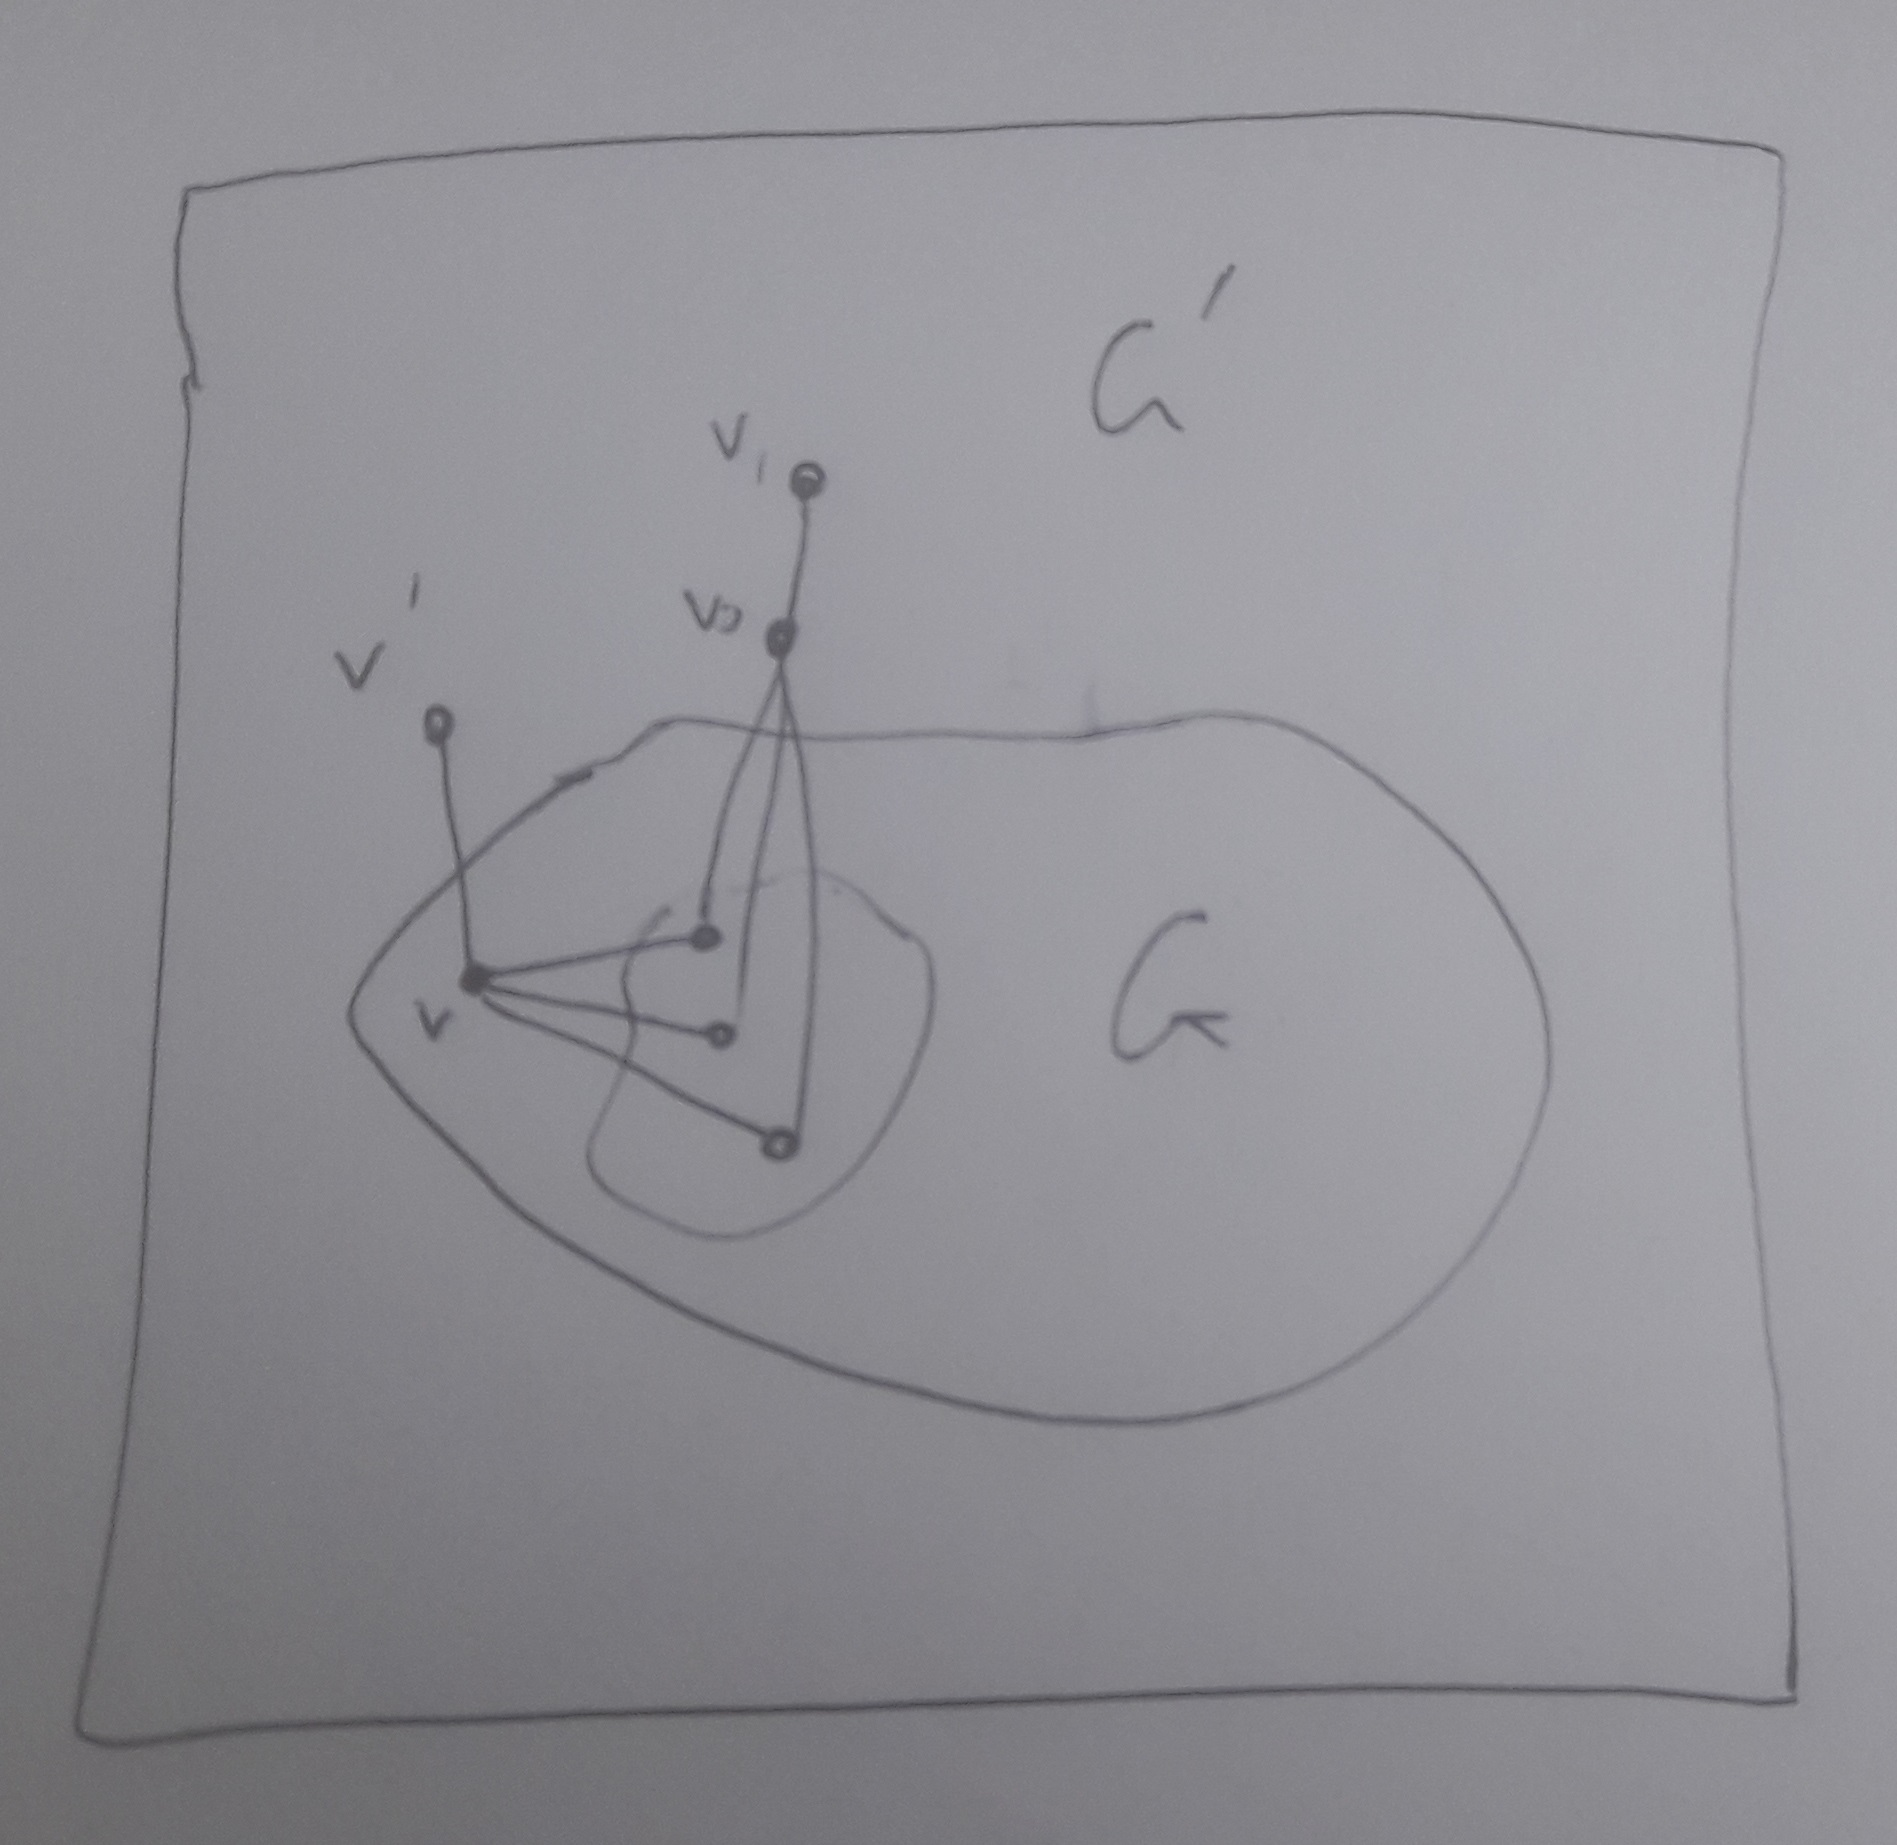
\includegraphics[scale = 0.1]{G.jpg}\]
Assume it takes constant time to choose a vertex $v$, and also that it takes constant time to create vertices. Then constructing the set of vertices of $G'$ is obviously $O(|V|)$. We add one edge to $G'$ for every edge of $G$, two edges $\{v,v'\}$ and $\{v_0,v_1\}$, and then an edge $\{v_0,u\}$ for every edge $\{v,u\}$ of $G$. As usual assuming constant time to create edges, this is $O(|E|) + O(|E|) = O(|E|)$. So the total time is $O(|V|+|E|)$.
Let $u_0,\ldots,u_n$ be a Hamiltonian circuit of $G$, and suppose without loss of generality that $u_0 = v$. Consider the sequence $v',v=u_0,\ldots,u_n,v_0,v_1$ of $G'$. There are obviously no repeated vertices in this sequence. Moreover, there are edges $\{v',v\}$ and $\{v_0,v_1\}$ by construction of $G'$, and, as there is an edge $\{u_n,u_0\}$ in $G$, there is also an edge $\{u_n, v_0\}$. It follows that $v',v,u_0,\ldots,u_n,v_0,v_1$ is a Hamiltonian path.

Conversely, suppose $u_0,u_1,\ldots,u_{m-1},u_m$ is a Hamiltonian path in $G'$. Then we can suppose without loss of generality that $u_0 = v'$, $u_1 = v$, $u_{m-1} = v_0$ and $u_m = v_1$ (as $v'$ and $v_1$ are the only possible endpoints of such a path). It follows that $u_1,\ldots,u_{m-2}$ is a Hamiltonian path in $G$. Moreover, as there is an edge $\{u_{m-2},u_{m-1}\}$ in $G'$ (i.e. from $u_{m-2}$ to $v_0$), there must be an edge $\{u_{m-2},u_1\}$ in $G$ (i.e. from $u_{m-2}$ to $v=u_1$). Thus $u_1,\ldots,u_{m-2}$ is a Hamiltonian circuit as required. 
We have defined a $p$-time reduction as required.

\end{comment}


\end{document}
\section*{$\NP$-Completeness}
\setcounter{Q}{0}
\documentclass{article}

\usepackage{amsmath, mathrsfs, amssymb, stmaryrd, cancel, relsize,tikz,amsthm,comment,enumerate}

\theoremstyle{definition}
\newtheorem{Q}{Question}
\newtheorem{definition}{Definition}

\newcommand{\tvs}{\textvisiblespace}
\newcommand{\ra}{\rightarrow}
\newcommand{\la}{\leftarrow}
\newcommand{\co}{\mathbf{code}}
\newcommand{\NP}{\mathbf{NP}}
\newcommand{\bbN}{\mathbb{N}}
\newcommand{\bbR}{\mathbb{R}}
\newcommand{\SAT}{\mathsf{PSAT}}

%\includecomment{comment}


\title{ITCS 532 Foundations of Computer Science\\
Week 8 Quiz}
\author{Rob Egrot}
\date{}

\begin{document}
\maketitle

\begin{Q}
Let $\Sigma = \{a,b\}$. Given $n\in \bbN$ let e.g. $a^n$ be the string that is the $a$ symbol $n$ times. For example, $b^3 = bbb$. Let $L=\{a^nb^n:n\in \bbN\setminus\{0\}\}$. Design a Turing machine that decides $L$. Express this machine as a state change diagram.  
\end{Q}
\begin{comment}
\textbf{Solution}
Undefined transitions can be considered to lead to the reject state. The idea is that $a$ is expected as the first symbol. If the 1st symbol is not $a$ then the machine rejects immediately. If it is $a$ then the machine erases it then looks for the last symbol, which it expects to be a $b$. If it is not a $b$ then the machine rejects. If it is a $b$ then the machine erases it and looks for the first non-blank symbol, which it expects to be $a$. If it is $a$ it erases it then looks for the last symbol, which it expects to be $b$, etc. This process of erasing the first $a$ and the last $b$ repeats. If the string has the right form then the machine will end up erasing the whole input and accepting. If it is not the right form then it will not see an $a$ or $b$ at some point when it expects to, and so will reject. Note that this algorithm could be made more efficient at the cost of a more complicated Turing machine.
\begin{center}
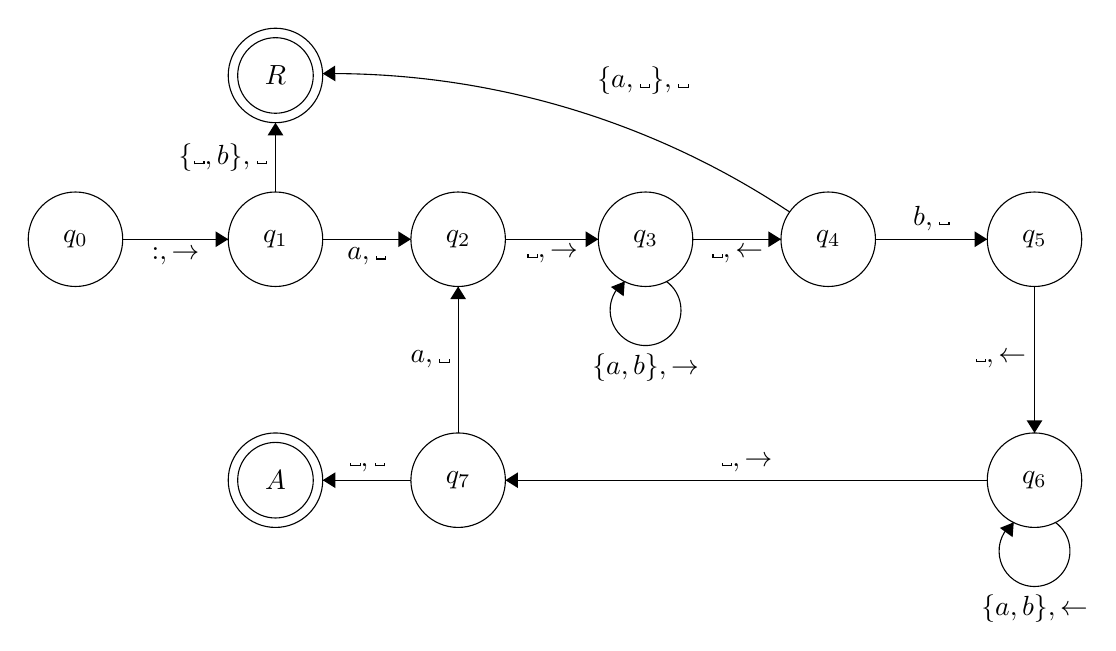
\begin{tikzpicture}[scale=0.2]
\tikzstyle{every node}+=[inner sep=0pt]
\draw [black] (7.5,-14) circle (3);
\draw (7.5,-14) node {$q_0$};
\draw [black] (20.2,-14) circle (3);
\draw (20.2,-14) node {$q_1$};
\draw [black] (20.2,-3.6) circle (3);
\draw (20.2,-3.6) node {$R$};
\draw [black] (20.2,-3.6) circle (2.4);
\draw [black] (31.8,-14) circle (3);
\draw (31.8,-14) node {$q_2$};
\draw [black] (43.7,-14) circle (3);
\draw (43.7,-14) node {$q_3$};
\draw [black] (55.3,-14) circle (3);
\draw (55.3,-14) node {$q_4$};
\draw [black] (68.4,-14) circle (3);
\draw (68.4,-14) node {$q_5$};
\draw [black] (68.4,-29.3) circle (3);
\draw (68.4,-29.3) node {$q_6$};
\draw [black] (20.2,-29.3) circle (3);
\draw (20.2,-29.3) node {$A$};
\draw [black] (20.2,-29.3) circle (2.4);
\draw [black] (31.8,-29.3) circle (3);
\draw (31.8,-29.3) node {$q_7$};
\draw [black] (10.5,-14) -- (17.2,-14);
\fill [black] (17.2,-14) -- (16.4,-13.5) -- (16.4,-14.5);
\draw (13.85,-14.5) node [below] {$:,\rightarrow$};
\draw [black] (20.2,-11) -- (20.2,-6.6);
\fill [black] (20.2,-6.6) -- (19.7,-7.4) -- (20.7,-7.4);
\draw (19.7,-8.8) node [left] {$\{\tvs,b\},\tvs$};
\draw [black] (23.2,-14) -- (28.8,-14);
\fill [black] (28.8,-14) -- (28,-13.5) -- (28,-14.5);
\draw (26,-14.5) node [below] {$a,\tvs$};
\draw [black] (34.8,-14) -- (40.7,-14);
\fill [black] (40.7,-14) -- (39.9,-13.5) -- (39.9,-14.5);
\draw (37.75,-14.5) node [below] {$\tvs,\rightarrow$};
\draw [black] (46.7,-14) -- (52.3,-14);
\fill [black] (52.3,-14) -- (51.5,-13.5) -- (51.5,-14.5);
\draw (49.5,-14.5) node [below] {$\tvs,\leftarrow$};
\draw [black] (23.197,-3.482) arc (90.62681:56.36446:52.499);
\fill [black] (23.2,-3.48) -- (24,-3.97) -- (23.99,-2.97);
\draw (43.54,-4.85) node [above] {$\{a,\tvs\},\tvs$};
\draw [black] (45.023,-16.68) arc (54:-234:2.25);
\draw (43.7,-21.25) node [below] {$\{a,b\},\rightarrow$};
\fill [black] (42.38,-16.68) -- (41.5,-17.03) -- (42.31,-17.62);
\draw [black] (58.3,-14) -- (65.4,-14);
\fill [black] (65.4,-14) -- (64.6,-13.5) -- (64.6,-14.5);
\draw (61.85,-13.5) node [above] {$b,\tvs$};
\draw [black] (68.4,-17) -- (68.4,-26.3);
\fill [black] (68.4,-26.3) -- (68.9,-25.5) -- (67.9,-25.5);
\draw (67.9,-21.65) node [left] {$\tvs,\leftarrow$};
\draw [black] (65.4,-29.3) -- (34.8,-29.3);
\fill [black] (34.8,-29.3) -- (35.6,-29.8) -- (35.6,-28.8);
\draw (50.1,-28.8) node [above] {$\tvs,\rightarrow$};
\draw [black] (69.723,-31.98) arc (54:-234:2.25);
\draw (68.4,-36.55) node [below] {$\{a,b\},\leftarrow$};
\fill [black] (67.08,-31.98) -- (66.2,-32.33) -- (67.01,-32.92);
\draw [black] (31.8,-26.3) -- (31.8,-17);
\fill [black] (31.8,-17) -- (31.3,-17.8) -- (32.3,-17.8);
\draw (31.3,-21.65) node [left] {$a,\tvs$};
\draw [black] (28.8,-29.3) -- (23.2,-29.3);
\fill [black] (23.2,-29.3) -- (24,-29.8) -- (24,-28.8);
\draw (26,-28.8) node [above] {$\tvs,\tvs$};
\end{tikzpicture}
\end{center}

\end{comment}

\begin{Q}
\mbox{}
\begin{enumerate}[a)]
\item Give an example of a formal language that is r.e. but not recursive.
\item Give an example of a formal language that is not r.e.
\end{enumerate}
\end{Q}
\begin{comment}
\textbf{Solution}
\begin{enumerate}[a)]
\item SA (see Definition \ref{D:SA}).
\item NSA (see Definition \ref{D:NSA}). 
\end{enumerate}
\end{comment}


\begin{Q}
\mbox{}
\begin{enumerate}[a)]
\item Prove that if a language $L$ and its complement $\bar{L}$ are both r.e. then $L$ is actually recursive.
\item Let $L$ be the language containing (in encoded form) all pairs $(M, w)$ such that $M$ is a Turing machine and $w$ is a string such that $M$ does \emph{not} halt on input $w$. Prove that $L$ is not r.e. HINT: Think about the halting problem and part a).   
\end{enumerate}
\end{Q}
\begin{comment}
\textbf{Solution}
\begin{enumerate}[a)]
\item Theorem \ref{T:comps}
\item Let $L'$ be the language consisting of $L$ together with all the finite strings which are not the coded form of a Turing machine and an input. Since it is decidable whether a string is the coded form of a Turing machine and an input (by the definition of encoding), $L'$ is r.e. if and only if $L$ is r.e. Note that $L'$ is the complement of the language consisting of the codes of $(T,I)$ such that $T(I)$ halts. This is the Halting problem, which we know is semidecidable but not decidable. Since the Halting problem is semidecidable, if $L'$ were r.e. then the Halting problem would be decidable, by part a). Since this is false, $L'$ and thus $L$ cannot be r.e.
\end{enumerate}
\end{comment}



\begin{Q}
Let $P$ be a property of finite strings over some fixed finite alphabet $\Sigma$ such that $P$ is true for least one finite string $s\in\Sigma^*$ (i.e. $P(s)$ holds). Let $D$ be the following decision problem: 

``Given a Turing machine $T$, does $T$ halt for every input $I$ such that $P(I)$ holds?"'.

Prove that $D$ is undecidable. HINT: prove $ETHP\leq D$.
\end{Q}
\begin{comment}
\textbf{Solution}
Let $T$ be a Turing machine (an instance of ETHP). Define the machine $M_T$ that operates as follows:
\begin{enumerate}
\item $M_T$ erases the input.
\item $M_T$ computes $T(\varepsilon)$.
\end{enumerate}
Since $M_T$ is a Turing machine, it is an instance of $D$. We need to show that the reduction is correct.
\begin{itemize}
\item Suppose $T(\varepsilon)$ halts. Then $M_T(I)$ halts for all $I$, so it certainly halts for all $I$ such that $P(I)$ holds. I.e. a yes instance of ETHP becomes a yes instance of $D$.
\item Conversely, suppose $T(\varepsilon)$ does not halt. Then, in particular, if $s\in\Sigma^*$ is chosen so that $P(s)$ holds, we have that $M_T(s)$ does not halt. I.e. a no instance of ETHP becomes a no instance of $D$. 
\end{itemize}
\end{comment}

\begin{Q}
\mbox{}
\begin{enumerate}[a)]
\item Let $k\in\bbN\setminus\{0\}$, and let $f:\bbR\to\bbR$ be a non-negative valued function (i.e. $f(x)\geq 0$ for all $x$). Show that $O(f(n))=O(kf(n))$. I.e. if $g$ is $O(f(n))$ then $g$ is also $O(kf(n))$, and vice versa.
\item Let $f,h:\bbR\to\bbR$ be non-negative valued functions, and suppose that there is $x_0\in\bbR$ such that $f(x)\leq h(x)$ for all $x\geq x_0$. Show that $O(f(n)+h(n))= O(h(n))$. I.e. if $g$ is $O(f(n)+h(n))$ then $g$ is also $O(h(n))$, and vice versa.
\end{enumerate}
\end{Q}
\begin{comment}
\textbf{Solution}
\begin{enumerate}[a)]
\item If $g$ is $O(f(n))$ there is a constant $c$ with $|g(n)|\leq cf(n)$ for large $n$. Clearly $|g(n)|\leq ckf(n)$ too, so $g$ is $O(kf(n))$. Conversely, if $g$ is $O(kf(n))$ there is a constant $c$ with $|g(n)|\leq ckf(n)$ for large $n$. But then $g$ is also $O(f(n))$ as we can use $ck$ for the constant. 
\item If $g$ is $O(f(n)+h(n))$ there is $c$ with $|g(n)|\leq c(f(n)+h(n))$ for all large $n$. By assumption, for large enough $n$ we also have $f(n)\leq h(n)$, so for values of $n$ that are `large' by both measures we have $|g(n)|\leq c(f(n)+h(n)) \leq 2ch(n)$. So $g$ is also $O(h(n))$, using the constant value $2c$. Conversely, if $|g(n)|\leq cf(n)$, then $|g(n)|\leq c(f(n)+h(n))$, as $f$ and $h$ are non-negative valued. So if $g$ is $O(h(n))$ it is also $O(f(n)+h(n))$. 
\end{enumerate}
\end{comment}


\begin{Q}
Recall Definition \ref{D:TSDP}. 
\begin{enumerate}[a)]
\item Show that $TSDP$ is in $\NP$ (HINT: describe a $p$-time verifier). 
\item Assuming that $HCP$ is $\NP$-complete, prove the converse of Theorem \ref{T:TSDPtoHCP} (i.e. that $TSDP\leq_p HCP$).
\end{enumerate}
\end{Q}
\begin{comment}
\textbf{Solution}
\begin{enumerate}[a)]
\item The certificates for the verifier are (coded forms of) sequences of vertices. The verifier checks if a given certificate defines a Hamiltonian circuit with an appropriate weight. It accepts if so, and rejects otherwise.
\item $TSDP\leq_p HCP$ by $NP$-hardness of $HCP$.
\end{enumerate}
\end{comment}

\begin{Q}\mbox{}
\begin{itemize}
\item A \emph{clique} in a graph $G$ is a set $C$ of vertices of $G$ such that every pair of distinct vertices in $C$ is connected by an edge. 
\item Let CLIQUE be the decision problem ``Given a graph $G$ and $k\in \bbN$, does $G$ contain a clique of size at least $k$?".
\item An \emph{independent set} in a graph $G$ is a set of vertices $I$ of $G$ such that no pair of vertices in $I$ is connected by an edge.
\item Let INDSET be the decision problem ``Given a graph $G$ and $k\in \bbN$, does $G$ contain an independent set of size at least $k$?".   
\end{itemize}
Prove that $CLIQUE \equiv_p INDSET$.
\end{Q}
\begin{comment}
\textbf{Solution}
Given a graph $G$, define the graph $\bar{G}$ to have the same vertices as $G$, and say there is an edge $\{u,v\}$ in $\bar{G}$ if and only if there is not an edge $\{u,v\}$ in $G$. This construction clearly takes $p$-time. Moreover, a clique/independent set of size $k$ in $G$ is an independent set/clique of size $k$ in $\bar{G}$, and vice versa. So this transformation maps yes instance of CLIQUE to yes instances of INDSET, and vice versa. So $CLIQUE \leq_p INDSET$ and $INDSET\leq_p CLIQUE$. I.e. $CLIQUE \equiv_p INDSET$.  
\end{comment}

\begin{Q}
Look at the proof of the fact that $\SAT$ is $\NP$-complete (Theorem \ref{T:cook}). Using the notation given in that proof, write down a Boolean formula $\psi$ that expresses that at some point the machine is in the accept state.
\end{Q}
\begin{comment}
\textbf{Solution}
Let $A$ be the accept state. Then $\psi = \bigvee_{1\leq i,j\leq Cn^k} p_{i,j,A}$.
\end{comment}





\end{document}


\begin{thebibliography}{1}

\bibitem{Sav98}
John Savage.
\newblock {\em Models of Computation}.
\newblock 1998.
\newblock URL: \url{http://cs.brown.edu/people/jsavage/book/}.

\bibitem{Sip12}
Michael Sipser.
\newblock {\em Introduction to the Theory of Compuation}.
\newblock 3rd edition, 2012.

\bibitem{SmithGod}
Peter Smith.
\newblock G\"odel without (too many) tears.
\newblock URL: \url{https://www.logicmatters.net/igt/godel-without-tears/}.

\end{thebibliography}

\bibliographystyle{plainurl}

\end{document}